\documentclass[
		11pt,
		a4paper,
		toc=listof, %% Abbildungs-, Tabellenverzeichnis mit ins Inhaltsverzeichni
		bibliography=totoc %% Quellenverzeichnis mit ins Inhaltsverzeichnis
		]{scrreprt}	 %% KOMA Script

% HTWG
\usepackage{graphicx}
\usepackage{a4}
\usepackage{german}

% Eigene
\usepackage[utf8]{inputenc} %% Umlaute
\usepackage[printonlyused]{acronym} %% Abkuerzungsverzeichnis (nur verwendete)
\usepackage{todonotes} %% TODOs moeglich mit \todo{}
\usepackage{listings} %% Codebeispiele
\usepackage{hyperref} %% referenzen innerhalb und außerhalb des Dokumentes
\usepackage[htt]{hyphenat} %% texttt umbrechen

% Eigenes Design
%TODO loeschen wenn default HTWG Design (was es nicht wirklich gibt) gewuenscht ist
\usepackage[bottom=3cm]{geometry}
\usepackage{setspace}
\onehalfspacing


% KOMA script anpassungen
%TODO entfernen wenn kein KOMA Script gewuenscht
\usepackage{scrhack}

% Codebeispiele
\usepackage{color}
\usepackage{xcolor}
\usepackage{listings}
\usepackage{caption}

% Inhaltsverzeichnis Abstaende
\usepackage{tocloft}
\setlength{\cftbeforechapskip}{4pt}

\usepackage{fancyvrb}
\newcommand{\VerbBar}{|}
\newcommand{\VERB}{\Verb[commandchars=\\\{\}]}
\DefineVerbatimEnvironment{Highlighting}{Verbatim}{commandchars=\\\{\},fontsize=\small,baselinestretch=1}
% Add ',fontsize=\small' for more characters per line
\newenvironment{Shaded}{}{}
\newcommand{\KeywordTok}[1]{\textcolor[rgb]{0.00,0.44,0.13}{\textbf{{#1}}}}
\newcommand{\DataTypeTok}[1]{\textcolor[rgb]{0.56,0.13,0.00}{{#1}}}
\newcommand{\DecValTok}[1]{\textcolor[rgb]{0.25,0.63,0.44}{{#1}}}
\newcommand{\BaseNTok}[1]{\textcolor[rgb]{0.25,0.63,0.44}{{#1}}}
\newcommand{\FloatTok}[1]{\textcolor[rgb]{0.25,0.63,0.44}{{#1}}}
\newcommand{\ConstantTok}[1]{\textcolor[rgb]{0.53,0.00,0.00}{{#1}}}
\newcommand{\CharTok}[1]{\textcolor[rgb]{0.25,0.44,0.63}{{#1}}}
\newcommand{\SpecialCharTok}[1]{\textcolor[rgb]{0.25,0.44,0.63}{{#1}}}
\newcommand{\StringTok}[1]{\textcolor[rgb]{0.25,0.44,0.63}{{#1}}}
\newcommand{\VerbatimStringTok}[1]{\textcolor[rgb]{0.25,0.44,0.63}{{#1}}}
\newcommand{\SpecialStringTok}[1]{\textcolor[rgb]{0.73,0.40,0.53}{{#1}}}
\newcommand{\ImportTok}[1]{{#1}}
\newcommand{\CommentTok}[1]{\textcolor[rgb]{0.38,0.63,0.69}{\textit{{#1}}}}
\newcommand{\DocumentationTok}[1]{\textcolor[rgb]{0.73,0.13,0.13}{\textit{{#1}}}}
\newcommand{\AnnotationTok}[1]{\textcolor[rgb]{0.38,0.63,0.69}{\textbf{\textit{{#1}}}}}
\newcommand{\CommentVarTok}[1]{\textcolor[rgb]{0.38,0.63,0.69}{\textbf{\textit{{#1}}}}}
\newcommand{\OtherTok}[1]{\textcolor[rgb]{0.00,0.44,0.13}{{#1}}}
\newcommand{\FunctionTok}[1]{\textcolor[rgb]{0.02,0.16,0.49}{{#1}}}
\newcommand{\VariableTok}[1]{\textcolor[rgb]{0.10,0.09,0.49}{{#1}}}
\newcommand{\ControlFlowTok}[1]{\textcolor[rgb]{0.00,0.44,0.13}{\textbf{{#1}}}}
\newcommand{\OperatorTok}[1]{\textcolor[rgb]{0.40,0.40,0.40}{{#1}}}
\newcommand{\BuiltInTok}[1]{{#1}}
\newcommand{\ExtensionTok}[1]{{#1}}
\newcommand{\PreprocessorTok}[1]{\textcolor[rgb]{0.74,0.48,0.00}{{#1}}}
\newcommand{\AttributeTok}[1]{\textcolor[rgb]{0.49,0.56,0.16}{{#1}}}
\newcommand{\RegionMarkerTok}[1]{{#1}}
\newcommand{\InformationTok}[1]{\textcolor[rgb]{0.38,0.63,0.69}{\textbf{\textit{{#1}}}}}
\newcommand{\WarningTok}[1]{\textcolor[rgb]{0.38,0.63,0.69}{\textbf{\textit{{#1}}}}}
\newcommand{\AlertTok}[1]{\textcolor[rgb]{1.00,0.00,0.00}{\textbf{{#1}}}}
\newcommand{\ErrorTok}[1]{\textcolor[rgb]{1.00,0.00,0.00}{\textbf{{#1}}}}
\newcommand{\NormalTok}[1]{{#1}}
\setlength{\parindent}{0pt}

\lstdefinelanguage{JavaScript}{
  keywords={typeof, new, true, false, catch, function, return, null, catch, switch, var, if, in, while, do, else, case, break},
  keywordstyle=\color{black}\bfseries,
  ndkeywords={class, export, boolean, throw, implements, import, this},
  ndkeywordstyle=\color{darkgray}\bfseries,
  identifierstyle=\color{black},
  sensitive=false,
  comment=[l]{//},
  morecomment=[s]{/*}{*/},
  commentstyle=\color{black}\ttfamily,
  stringstyle=\color{black}\ttfamily,
  morestring=[b]',
  morestring=[b]"
}

\setcounter{tocdepth}{2}  %% Uebreschriften bis subsectionw ins Inhaltsverzeichnis
\setcounter{secnumdepth}{2}  %% Nummerierung bis subsection


%%% Codebeispiele - Style
\lstdefinestyle{mystyle}{
    basicstyle=\footnotesize,
    aboveskip=10pt,
    breakatwhitespace=false,
    breaklines=true,
    captionpos=b,
    belowcaptionskip=5pt,
    keepspaces=true,
    numbers=left,
    numbersep=15pt,
    showspaces=false,
    showstringspaces=false,
    showtabs=false,
    tabsize=2,
    frame=single,
    lineskip=-0.4pt,
    framexleftmargin=0.5em,
    xleftmargin=2.5em
}
\lstset{style=mystyle}


% Entfernt Kapitel Ueberschrift
% Bsp.
% 	ALT:
%       Kapitel 1
%       Einführung
%
% 	NEU:
% 		1 Einführung
%
\renewcommand*\chapterheadstartvskip{\vspace{-\topskip}}


% Hurenkind und Schusterjunge vermeiden
\clubpenalty = 10000 % schliesst Schusterjungen aus
\widowpenalty = 10000 \displaywidowpenalty = 10000% schliesst Hurenkinder aus


% Alle Listen mit einem "-" statt einem Punkt
\def\labelitemi{--}


\newcommand{\thema}{$[$Thema der Bachelorarbeit$]$}
\newcommand{\schlagworte}{$[$Platz, f\"ur, spezifische, Schlagworte, zur, Ausarbeitung $]$}
\newcommand{\zusammenfassung}{$[$Text der Zusammenfassung etwa 150 Worte. Es soll der
	L"osungsweg beschrieben sein.$]$}
\newcommand{\ausgabedatum}{$[$Datum$]$}
\newcommand{\abgabedatum}{15.02.2016}
\newcommand{\autor}{Sandro Tonon}
\newcommand{\autorStrasse}{Allemannenstra"se 10}
\newcommand{\autorPLZ}{78467}
\newcommand{\autorOrt}{Konstanz}
\newcommand{\autorGeburtsort}{Waldshut-Tiengen}
\newcommand{\autorGeburtsdatum}{02.07.1990}
\newcommand{\prueferA}{Prof. Dr. Marko Boger}
\newcommand{\prueferB}{Dipl. Ing. Andreas Maurer}
\newcommand{\firma}{Seitenbau GmbH}
\newcommand{\studiengang}{Angewandte Informatik}



\begin{document}
%% Nummerierung aus
\pagenumbering{gobble}

% HTWG Tempaltes fuer Titelseite etc.

\begin{titlepage}

\vspace*{-3.5cm}

\begin{flushleft}
\hspace*{-1cm} 
\includegraphics[width=15.7cm]{htwg-logo}
\end{flushleft}

\vspace{2.5cm}

\begin{center}
	\huge{
		\textbf{\thema} \\[5cm]
	}
	\Large{
		\textbf{\autor}} \\[6.5cm]
	\large{
		\textbf{Konstanz, \abgabedatum} \\[2.3cm]
	}
	
	\Huge{
		\textbf{{\sf BACHELORARBEIT}}
	}
\end{center}

\end{titlepage}

\thispagestyle{empty}
{
\setlength{\parskip}{0.5cm}
        \begin{center}
        \textbf{\huge BACHELORARBEIT}

        \textbf{zur Erlangung des akademischen Grades}

        \textbf{\Large Bachelor of Science (B. Sc.)}

        \textbf{an der}

        \textsf{\huge Hochschule Konstanz}\\
        {\small Technik, Wirtschaft und Gestaltung}

        \textsf{\Large Fakult"at Informatik} \\
        Studiengang \studiengang
        \end{center}
}
\begin{center}

\vspace*{2cm}

\begin{tabular}{p{3cm}p{10cm}}
Thema: & \multicolumn{1}{l}{\textbf{\large \thema}} \\[15ex]
Bachelorkandidat: & \autor, \autorStrasse, \autorPLZ{}  \autorOrt{} \\[15ex]
1. Pr"ufer: & \prueferA \\
2. Pr"ufer: & \prueferB \\[25ex]
Ausgabedatum: & \ausgabedatum \\
Abgabedatum: & \abgabedatum \\
\end{tabular}
\end{center}

\begin{center}
{\Large \textbf{Zusammenfassung (Abstract)}}
\end{center}

\bigskip

\begin{center}
	\begin{tabular}{p{2.8cm}p{10cm}}
		Thema: & \thema \\
		 & \\
		Bachelorkandidat: & \autor \\
		 & \\
		Firma: & \firma \\
		 & \\
		Betreuer: & \prueferA  \\[.5ex]
		 &  \prueferB \\
		 & \\
		Abgabedatum: & \abgabedatum \\
		 & \\
		Schlagworte: & \schlagworte \\
		 & \\
	\end{tabular}
\end{center}

\bigskip

\noindent
\zusammenfassung

\pagenumbering{Roman}
\chapter*{Ehrenw"ortliche Erkl"arung}
\addcontentsline{toc}{chapter}{Ehrenw"ortliche Erkl"arung}

Hiermit erkl"are ich
\textit{\autor, geboren am \autorGeburtsdatum{} in \autorGeburtsort{}}, dass ich\\

\begin{tabular}{lp{12cm}}
(1) & meine Bachelorarbeit mit dem Titel \\[1em]
& \textbf{\thema} \\[1em]
& selbstst"andig und ohne fremde Hilfe angefertigt und keine anderen als die angef"uhrten Hilfen benutzt habe;\\[1em]
(2) & die "Ubernahme w"ortlicher Zitate, von Tabellen, Zeichnungen, Bildern und
Programmen aus der Literatur oder anderen Quellen (Internet) sowie die Verwendung
der Gedanken anderer Autoren an den entsprechenden Stellen innerhalb der Arbeit
gekennzeichnet habe.\\
\end{tabular}

\vspace*{1cm}

\noindent
Ich bin mir bewusst, dass eine falsche Erkl"arung rechtliche Folgen haben wird.\\

\vspace*{3cm}

\noindent
Konstanz, \abgabedatum \hfill \begin{tabular}{c} \\ \\ \rule{5cm}{1pt} \\ (Unterschrift)\end{tabular}


\tableofcontents

%% Starte Paginierung
\cleardoublepage
\pagenumbering{arabic}

\chapter{Einleitung}\label{einleitung}

Der Begriff ``Web Components'' ist ein Dachbegriff für mehrere entstehende Standards \cite{citeulike:13844988}, welche es für Webentwickler ermöglichen sollen, komplexe Anwendungsentwicklungen mit einer neuen Sammlung an Werkzeugen zu vereinfachen. Diese sollen die Wartbarkeit, Interoperabilität und Kapselung verbessern und somit ein Plugin-System für das Web schaffen. Durch die neuen Standards soll das Web zu einer Plattform werden, die es ermöglicht, die Web-Sprache \ac{HTML} zu erweitern. Dies ist bisher nicht möglich, da die \ac{HTML}-Technologie - und somit die Möglichkeiten, \ac{HTML}-Tags zu benutzen - vom \ac{W3C} definiert und standardisiert wird. Unter den wichtigsten der neuen Standards sind die folgenden 4 Technologien aufzuführen: Custom Elements, Shadow \ac{DOM}, \ac{HTML} Templates und \ac{HTML} Imports. Custom Elements ermöglichen es einem Webentwickler, eigene \ac{HTML}-Tags und deren Verhalten zu definieren, oder bereits vorhandene oder native \ac{HTML}-Tags zu erweitern. Das Shadow \ac{DOM} stellt ein Sub-\ac{DOM} in einem \ac{HTML}-Element bereit, welches dem Element zugehöriges Markup, \ac{CSS} und JavaScript kapselt. \ac{HTML} Templates stellen, wie der Name impliziert, einen Template-Mechanismus für \ac{HTML} bereit und \ac{HTML} Imports erlauben das Laden von \ac{HTML}-Dokumenten in andere \ac{HTML}-Dokumente. \cite{citeulike:13842702}, \cite{citeulike:13842701}

Diese neuen Technologien werden allerdings noch nicht vollständig von allen populären Browsern, zu welchen Google Chrome, Mozilla Firefox, Opera und der Internet Explorer bzw. Edge, gehören, unterstützt. Des Weiteren ist das Implementieren einer Applikation, welche diese Technologien nativ benutzt, bisher sehr komplex und schwierig zu organisieren. Im Zuge dessen, entwickelt Google aktiv an einer Library namens Polymer, welche sich diesen Problemen annimmt.
Polymer stellt dabei eine Reihe an unterschiedlichen Schichten dar, welche den Umgang mit Web Components vereinfachen sollen. So stellt Polymer eine Sammlung an Mechanismen bereit, welche älteren Browsern die nötigen Features für den Einsatz von Web Components beibringen. Ebenso soll das Erstellen von eigenen \ac{HTML}-Elementen mit der Polymer-Library und der damit bereitgestellten \ac{API} für Entwickler komfortabler gemacht werden. Um bereits entwickelte Web Components einfach wiederverwenden zu können, bietet Polymer eine Sammlung von vorgefertigten Elementen an.

Web Components und die Polymer-Library greifen stark in den Entwicklungsprozess von Webseiten ein und sollen diesen verbessern und vereinfachen. Die Seitenbau GmbH interessiert sich stark für diese neue Technologie, da Wiederverwendbarkeit, Wartbarkeit und neue Technologien im Fokus des Frontend-Engineerings des Unternehmens stehen.
Die Seitenbau GmbH ist ein mittelständischer IT-Dienstleister und unterstützt seit 1996 Organisationen aus Privatwirtschaft und öffentlicher Verwaltung bei der Planung, Konzeption und Umsetzung hochwertiger Softwarelösungen für E-Business und E-Government. Zu den Kernkompetenzen der Seitenbau GmbH zählen dabei vor allem das Frontend Engineering und Content Management, die Konzeption und Entwicklung von Individualsoftware sowie der Aufbau von personalisierten Intranet- und Portallösungen.

Im Rahmen dieser Bachelorarbeit sollen die verschiedenen Technologien unter dem Dachbegriff Web Components sowie deren Funktionsweise sowohl ohne, als auch mit der Polymer-Library, untersucht werden. Zur Veranschaulichung soll eine Web Component mit Hilfe von Polymer implementiert und mit einer ähnlichen Implementierung mit AngularJS verglichen werden. Am Beispiel einer Web Component in Form einer Multi-Navigations-Applikation sollen die Vor- und Nachteile des Einsatzes von Polymer in Hinblick auf Implementierung und Performance dargestellt werden.

In Kapitel \ref{web-components-nach-w3c} werden die Standards der Web Components beschrieben, auf welche die in Kapitel \ref{einfuehrung-in-polymer} beschriebene Library Polymer aufsetzt. Wie sie dies im Detail umsetzt wird in Kapitel \ref{analogie-zu-nativen-web-components} beschrieben. In Kapitel \ref{zusaetzliche-polymer-funktionalitaeten} werden zusätzliche Funktionalitäten dieser Library aufgezeigt und in Kapitel \ref{best-practices-beim-arbeiten-mit-polymer} werden einige Best Practices im Umgang mit ihr erklärt. Die in den Kapiteln \ref{einfuehrung-in-polymer} bis \ref{best-practices-beim-arbeiten-mit-polymer} gewonnenen Erkenntnisse werden in Kapitel \ref{komponenten-entwicklung} in einer Beispielimplementierung umgesetzt und mit einer ähnlichen Implementierung mit AngularJS verglichen. In Kapitel \ref{zukunftsprognose} wird abschließend eine Zukunftsprognose aufgestellt.


\chapter{Web Components nach dem vorläufigen W3C-Standard}\label{web-components-nach-w3c}

In diesem Kapitel wird in Abschnitt \ref{problemloesung} auf die Problemlösung der Web Components nach den Vorstellungen des \ac{W3C} eingegangen. In Abschnitt \ref{custom-elements} wird die erste Technologie vorgestellt, die Custom Elements, Abschnitt \ref{html-templates} wird sich den \ac{HTML} Templates widmen, in Abschnitt \ref{shadow-dom} wird auf den Shadow \ac{DOM} eingegangen und in Abschnitt \ref{html-imports} wird die letzte Technologie, die \ac{HTML} Imports, gezeigt. In Abschnitt \ref{polyfills-mit-webcomponents.js} werden die, für diese Technologien entwickelten Polyfills erklärt. Abschließend wird in Kapitel \ref{implementierung-einer-komponente-mit-den-nativen-web-component-apis} eine exemplarische Komponente implementiert.


\section{Problemlösung}\label{problemloesung}

In der heutigen Webentwicklung kommt es häufig vor, dass für diverse Probleme oftmals die gleiche, oder eine ähnliche Lösung entwickelt werden muss. Diese unterscheiden sich stets leicht, bringen im Kern aber dennoch meist die selben Features mit sich. Um diese Features auf der Webseite verfügbar zu machen, sind eine Reihe an verschiedenen Technologien notwendig. Zum einen muss das von ihr benötigte \ac{HTML}-Markup geschrieben werden, zum anderen muss ein JavaScript eingebunden und über eine vorgegebene \ac{API} konfiguriert werden, damit das Feature überhaupt funktioniert. Damit die Komponente dann in das Design der eigenen Webseite einfügt, muss ebenso ein entsprechendes Stylesheet mit den Style-Definitionen eingebunden werden. Da \ac{CSS}-Regeln immer global auf das gesamte Dokument angewendet werden, kann es dabei zu ungewollten Auswirkungen auf andere Bestandteile der Webseite kommen. Nimmt man diese Punkte zusammen, so wird deutlich, dass es in der Webentwicklung kein Plugin-System gibt um Webseiten schnell und einfach zu erweitern.

Diesem Problem widmen sich die Web Components. Sie sollen der Frontend-Entwicklung ein Plugin-System bereitstellen, welches diese Probleme löst. Eine Komponente steht dabei als eigenes \ac{HTML}-Element, welches ihre gesamte Funktionalität kapselt und nach außen verbirgt. Konflikte mit anderen Komponenten oder der einbindenden Webseite selbst werden somit vermieden. Dabei ist das Verhalten nach außen für jede Komponente dasselbe, es gibt also für jede Komponente die gleiche Schnittstelle, um sie zu konfigurieren und einzubinden. Dies erleichtert deren Umgang deutlich, da die einzige benötigte Technologie \ac{HTML} ist. Dadurch können Komponenten verwendet werden wie jedes native \ac{HTML}-Element. Sie sind verschachtelbar und haben Attribute, über welche sie konfiguriert werden können. Web Components bilden dabei eine Sammlung an Technologien, um jene Eigenschaften zu gewährleisten. In den folgenden Abschnitten werden diese Technologien erklärt und auf ihre Anwendung eingegangen.

\section{Custom Elements}\label{custom-elements}

Webseiten werden mit sogenannten Elementen, oder auch Tags, aufgebaut. Das Set an verfügbaren Elementen wird vom \ac{W3C} definiert und standardisiert. Somit ist die Auswahl an den verfügbaren Elementen stark begrenzt und nicht von Entwicklern erweiterbar, sodass diese nicht ihre eigenen, von ihrer Applikation benötigten Elemente, definieren können. Betrachtet man in Abbildung \ref{fig:cusel} den Quelltext einer populären Web-Applikation Google Mail, wird schnell deutlich, worin das Problem liegt.

\begin{figure}[htbp]
 \centering
 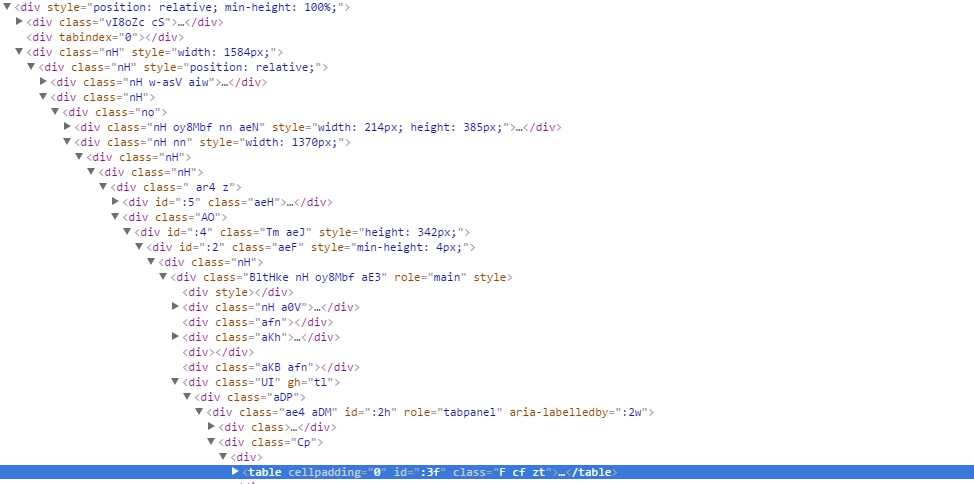
\includegraphics[width=14cm]{kapitel2/bilder/2-custom-elements-div-suppe}
 \caption{Screenshot des DOMs der Applikation Google Mail}
 \label{fig:cusel}
\end{figure}

Sie besteht aus vielen geschachtelten \texttt{\textless{}div\textgreater{}}-Elementen und macht folgende strukturelle Probleme deutlich: Die Semantik der Elemente fehlt vollständig und es ist nicht ersichtlich was es darstellt und welche Funkionen es hat, wodurch die Applikation nur sehr schwer wartbar ist.

Dieser Problematik widmen sich die Custom Elements. Sie bieten eine neue \ac{API}, welche es ermöglicht, eigene, semantisch aussagekräftige \ac{HTML}-Elemente mit Eigenschaften und Funktionen zu definieren. Wird das obige Beispiel nun also mit Hilfe von Custom Elements umgesetzt, so könnte das zugehörige \ac{DOM} wie in Listing \ref{beamwc} dargestellt aussehen \cite{citeulike:13844982}.

\lstinputlisting[language=HTML,label=beamwc,caption=Beispiel einer Applikation mit Web Components]{kapitel2/listings/2-1.html}

Die Spezifikation des \ac{W3C} ermöglicht nicht nur das Erstellen eigenständiger Elemente, sondern auch das Erstellen von Elementen, welche native Elemente erweitern. Somit können die \ac{API}s von nativen \ac{HTML}-Elementen um eigene Eigenschaften und Funktionen erweitert werden.


\subsection{Neue Elemente registrieren}\label{neue-elemente-registrieren}

Um nun ein eigenes Custom Element zu definieren, muss der Name des Custom Elements laut der \ac{W3C}-Spezifikation zwingend einen Bindestrich enthalten, wie beispielsweise in \texttt{my-element}. Somit ist gewährleistet, dass der Parser des Browsers die Custom Elements von den nativen Elementen unterscheiden kann \cite{citeulike:13845061}. Ein neues Element wird mittels JavaScript mit der Funktion \texttt{document.registerElement('my-element');} registriert. Zusätzlich zum Namen des Elements kann optional der Prototyp des Elements angegeben werden. Dieser ist jedoch standardmäßig ein \texttt{HTMLElement}, somit also erst wichtig, wenn es darum geht, vorhandene Elemente zu erweitern (siehe Abschnitt \ref{vorhandene-elemente-erweitern-type-extensions}). Durch das Registrieren des Elements wird es in die Registry des Browsers geschrieben, welche dazu verwendet wird, die Definitionen der \ac{HTML}-Elemente aufzulösen \cite{citeulike:13844982}. Ist ein Element noch nicht definiert und nicht beim Browser registriert, steht aber im Markup der Webseite, wird dies keinen Fehler verursachen, da dieses Element das Interface von \texttt{HTMLUnkownElement} benutzen muss \cite{citeulike:13851253}.

Nachdem das Element beim Browser registriert wurde, muss es zunächst mittels der Anweisung \texttt{document.createElement(tagName);} erzeugt werden, der \texttt{tagName} ist hierbei der Name des zuvor registrierten Elements. Danach kann es imperativ per JavaScript mittels \texttt{document.body.appendChild(myelement);} oder deklarativ direkt im \ac{HTML}-Dokument mittels \texttt{\textless{}my-element\textgreater{}\textless{}my-element\textgreater{}} verwendet werden.

\noindent \cite[S. 127-138]{citeulike:13844975}


\subsection{Vorhandene Elemente erweitern (Type Extensions)}\label{vorhandene-elemente-erweitern-type-extensions}

Statt neue Elemente zu erzeugen, können sowohl native \ac{HTML}-Elemente als auch bereits erstellte Custom Elements durch prototypische Vererbung um Funktionen und Eigenschaften erweitert werden, was auch als ``Type Extension'' bezeichnet wird. Zusätzlich zum Namen des erweiterten Elements wird nun der Prototyp sowie der Name des zu erweiternden Elements der \texttt{registerElement}-Funktion als Parameter übergeben. Soll also ein erweitertes \texttt{button}-Element registriert werden, muss dies wie in Listing \ref{reebe} gemacht werden.

\lstinputlisting[language=JavaScript,label=reebe,caption=Registrieren eines erweiterten Button-Elements]{kapitel2/listings/2-2.js}

Das registrierte, erweiterte Element kann nun mit dem Namen des zu erweiternden Elements als erstem Parameter und dem Namen des erweiterten Elements als zweitem Parameter erzeugt werden. Alternativ kann es auch mit Hilfe des Konstruktors erzeugt werden (siehe Listing \ref{eeebe}) \cite{citeulike:13752379}.

\lstinputlisting[language=HTML,label=eeebe,caption=Erzeugen eines erweiterten Button-Elements]{kapitel2/listings/2-3.js}

Um es nun im \ac{DOM} zu benutzen, muss der Name des erweiterten Elements via dem Attribut \texttt{is=\dq elementName\dq} des erweiternden Elements angegeben werden. So wird der erweiterte Button deklarativ mittels \texttt{\textless{}button\ is=\dq button-extended\dq\textgreater{}\textless{}/button\textgreater{}} in das Dokument eingebunden.


\subsection{Eigenschaften und Methoden definieren}\label{eigenschaften-und-methoden-definieren}

Anhand des obigen Beispiels wird deutlich, wie ein Custom Element eingesetzt werden kann, jedoch sind die internen JavaScript-Mechanismen nicht ersichtlich. Custom Elements entfalten ihr vollständiges Potential jedoch erst, wenn man für diese auch eigene Eigenschaften und Methoden definiert. Wie bei nativen \ac{HTML}-Elementen ist das auch bei Custom Elements auf analoge Weise möglich \cite[S. 127-138]{citeulike:13844975}. So kann einem Element eine Funktion zugewiesen werden, in dem diese dessen Prototyp mittels einem nicht reservierten Namen angegeben wird. Selbiges gilt für eine neue Eigenschaft. Die Eigenschaften können, nachdem sie im Prototyp definiert wurden, im \ac{HTML}-Markup deklarativ konfiguriert werden (siehe Listing \ref{eumduk}). Eigene Elemente mit einem spezifischen Eigenverhalten und Aussehen, wie beispielsweise ein neuer Video-Player, sind dadurch mit einem Tag statt mit einem Gerüst aus \texttt{\textless{}div\textgreater{}}-Tags oder Ähnlichem umsetzbar.

\lstinputlisting[language=HTML,label=eumduk,caption=Eigenschaften und Methoden definieren und konfigurieren]{kapitel2/listings/2-4.html}


\subsection{Custom Element Lifecycle-Callbacks}\label{custom-element-lifecycle-callbacks}

Custom Elements bieten eine standardisierte \ac{API} an speziellen Methoden, den ``Custom Element Lifecycle-Callbacks'', welche es ermöglichen Funktionen zu unterschiedlichen Zeitpunkten - vom Registrieren bis zum Löschen eines Custom Elements - auszuführen. Diese ermöglichen es, zu bestimmen, wann und wie ein bestimmter Code des Custom Elements ausgeführt werden soll.

\begin{description}
  \item[createdCallback] Wird ausgeführt, wenn eine Instanz des Custom Elements mittels \texttt{var\ mybutton\ =\ document.createElement('custom-element')} erzeugt wurde.
  \item[attachedCallback] Wird ausgeführt, wenn ein Custom Element dem \ac{DOM} mittels der Funktion \texttt{document.body.appendChild(mybutton)} angehängt wurde.
  \item[detachedCallback] Wird ausgeführt, wenn ein Custom Element aus dem \ac{DOM} mittels der Funktion \texttt{document.body.removeChild(mybutton)} entfernt wurde.
  \item[attributeChangedCallback] Wird ausgeführt, wenn ein Attribut eines Custom Elements mittels \texttt{MyElement.setAttribute()} geändert wurde.
\end{description}

So können die Lifecycle-Callbacks für ein neues erweitertes Button-Element, wie in Listing \ref{lccdebd} dargestellt, definiert werden \cite{citeulike:13844988}.

\lstinputlisting[language=HTML,label=lccdebd,caption=Lifecycle-Callbacks des erweiterten Buttons definieren]{kapitel2/listings/2-5.html}


\subsection{Styling von Custom Elements}\label{styling-von-custom-elements}

Das Styling von eigenen Custom Elements funktioniert analog dem Styling von nativen \ac{HTML}-Elementen indem der Name des Elements als \ac{CSS}-Selektor angegeben wird (siehe Listing \ref{seceudeb}). Erweiterte Elemente können mittels dem Attribut-Selektor in \ac{CSS} angesprochen werden \cite[S. 127-138]{citeulike:13844975}.


Ein Custom Element, welches zwar standardkonform deklariert oder erstellt, aber noch nicht beim Browser registriert wurde, ist ein ``Unresolved Element''. Steht dieses Element am Anfang des \ac{DOM}, wird jedoch erst später registriert, kann es nicht von \ac{CSS} angesprochen werden. Dadurch kann ein \ac{FOUC} entstehen, was bedeutet, dass das Element beim Laden der Seite nicht gestylt dargestellt wird, sondern das definierte Aussehen erst übernimmt, nachdem es registriert wurde. Um dies zu verhindern, sieht die \ac{HTML}-Spezifikation eine neue \ac{CSS}-Pseudoklasse \texttt{:unresolved} (siehe Listing \ref{seceudeb}) vor, welche deklarierte, aber nicht registrierte Elemente anspricht. Somit können diese Elemente initial beim Laden der Seite ausgeblendet und nach dem Registrieren wieder eingeblendet werden \cite{citeulike:13844984}.

\lstinputlisting[language=HTML,label=seceudeb,caption=Styling eines Custom Element und des erweiterten Button]{kapitel2/listings/2-6.css}

\subsection{Browserunterstützung}\label{custom-elements-browserunterstuetzung}

Custom Elements sind noch nicht vom \ac{W3C} standardisiert, sondern befinden sich noch im Status eines ``Working Draft'' \cite{citeulike:13845061}. Sie werden deshalb bisher nur von Google Chrome ab Version 43 und Opera ab Version 33 nativ unterstützt (siehe Abbildung \ref{fig:buce}) \cite{citeulike:13844983}.

\begin{figure}[htbp]
 \centering
 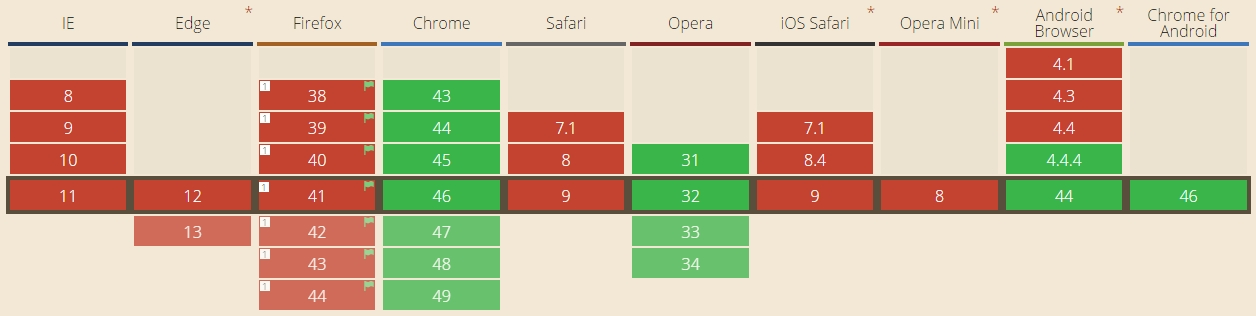
\includegraphics[width=\linewidth]{kapitel2/bilder/2-custom-elements-browserunterstuetzung}
 \caption{Browserunterstützung von Custom Elements}
 \label{fig:buce}
\end{figure}

\section{HTML Templates}\label{html-templates}

\todo{Buchquelle hinzufügen [S.101-107]} Bisher gibt es ohne eine Library oder Framework keine Möglichkeit, im Browser Templates zu rendern, um bestimmte Inhalte der Seite zur Laufzeit auszuwechseln. Die Technologie ``\ac{HTML} Templates'' ist eine neue Technologie im Rahmen der Web Components und versucht eben dieses Problem mit einer nativen \ac{API} zu lösen.

Im Kontext der Entwicklung einer \ac{MVC}-Applikation ist der Mechanismus der Darstellung der Präsentations-Schicht, auch View genannt, besonders wichtig. Bisher ist dies ohne weiteres problemlos serverseitig in PHP, Ruby oder ähnlichem möglich, da diese Sprachen für die Webentwicklung eine Syntax für die Einbettung dynamischer Inhalte in \ac{HTML} bieten, die sogenannten Templates. Im Gegensatz zu den serverseitigen Technologien, existieren Client-seitige Lösungen bisher nur als Library oder Framework, wie beispielsweise Mustache.js oder Handlebars.js \cite{citeulike:13853015}. Eine native Möglichkeit, Templates auf der Client-Seite zu benutzen, fehlt bisher hingegen. An diese Problematik setzen die \ac{HTML} Templates an, durch welche diese Technik auch Einzug in den Browser erhält.

\begin{quote}
Das \ac{HTML} template-Element \textless{}template\textgreater{} dient dazu, Client-seitige Inhalte zu gruppieren, die nicht gerendert werden, wenn die Seite geladen wird, sondern anschließend zur Laufzeit mittels JavaScript gerendert werden können. Template kann als Inhaltsfragment aufgefasst werden, das für eine spätere Verwendung im Dokument gespeichert wird. \cite{citeulike:13852997}
\end{quote}


\subsection{Bisherige Umsetzung von Templates im Browser}\label{bisherige-umsetzung-von-templates-im-browser}

Dennoch gibt es diverse Methoden, diese Technologie im Browser zu simulieren. Diese sind jedoch eher als Hacks zu betrachten, da ihre eingesetzten Mittel nicht für dieses Problem gedacht sind. Sie bringen also einige Nachteile mit sich. Einige dieser Methoden werden nachfolgend aufgezeigt \cite{citeulike:13853018}.

\subsubsection{Via verstecktem \texttt{\textless{}div\textgreater{}}-Element}

Das Listing \ref{uetmedb} zeigt die Umsetzung eines Templates mit Hilfe eines \texttt{\textless{}div\textgreater{}}-Blocks, der via \ac{CSS} versteckt wird.

\lstinputlisting[language=HTML,label=uetmedb,caption=Umsetzung eines Templates mit einem \texttt{\textless{}div\textgreater{}}-Block]{kapitel2/listings/4-1.html}

Der Nachteil dieser Methode ist, dass alle enthaltenen Ressourcen, beim Laden der Webseite heruntergeladen werden. Zwar werden sie nicht angezeigt, dennoch verursachen sie eine große Datenmenge, welche initial übertragen werden muss. Dies geschieht selbst wenn die Ressourcen eventuell erst später oder gar nicht benötigt werden. Des Weiteren kann es sich als schwierig erweisen, ein solches Code-Fragment zu stylen oder gar Themes auf mehrere solcher Fragmente anzuwenden. Eine Webseite, die das Template verwendet, muss alle \ac{CSS}-Regeln für das Template mit \texttt{\#mydivtemplate} erstellen, welche sich unter Umständen auf andere Teile der Webseite auswirken können. Eine der Inhalts leistet diese Methode nicht.

\subsubsection{Via \texttt{\textless{}script\textgreater{}}-Element}

Eine weitere Möglichkeit ein Template umzusetzen besteht darin, den Inhalt eines Templates in ein \texttt{\textless{}script\textgreater{}}-Tag zu schreiben, wie in Listing \ref{uetmese} gezeigt.

\lstinputlisting[language=HTML,label=uetmese,caption=Umsetzung eines Templates mit einem \texttt{\textless{}script\textgreater{}}-Element]{kapitel2/listings/4-2.html}

Wie bei dem Beispiel mit einem \texttt{\textless{}div\textgreater{}}-Element wird auch bei dieser Methode der Inhalt nicht gerendert, da ein \texttt{\textless{}script\textgreater{}}-Tag standardmäßig die \ac{CSS}-Eigenschaft \texttt{display:\ none} hat. In diesem Fall werden jedoch die benötigten Ressourcen nicht geladen, somit gibt es keine zusätzlichen Performance-Einbrüche. Es besteht dennoch der Nachteil, dass der Inhalt des \texttt{\textless{}script\textgreater{}}-Tags via \texttt{innerHTML} in den \ac{DOM} geklont werden muss, was eine mögliche \ac{XSS} Sicherheitslücke darstellt. Es muss also abgewägt werden, welche der Nachteile für den Entwickler am ehesten hinnehmbar sind und welche Methode verwendet werden soll.


\subsection{Das \texorpdfstring{\texttt{\textless{}template\textgreater{}}-Tag}{\textless{}template\textgreater{}-Tag}}\label{template-tag}

Den Problemen der oben genannten Methoden widmet sich das \texttt{\textless{}template\textgreater{}}-Tag, welches eine native und sichere Methode für das Einbinden von dynamischen Inhalten etabliert. Das Template und die darin enthaltenen Inhalte bilden ein \ac{HTML}-Gerüst, welches beim Rendern des Webseite vollständig ignoriert wird. Es wird weder angezeigt, noch werden ihre benötigten Inhalte beim Laden der Webseite übertragen. Dadurch können beliebig viele \texttt{\textless{}template\textgreater{}}-Tags ohne signifikanten Performance-Einbruch im Quelltext stehen, da nur ihr Markup übertragen wird, es jedoch nicht vom Browser geparst werden muss, was erst beim Einfügen des Templates in das \ac{DOM} mittels JavaScript geschieht. Die Templates können dabei beliebig oft und an beliebiger Stelle in den \ac{DOM} der Webseite eingefügt werden. Des weiteren werden in Templates enthaltene JavaScripts nicht ausgeführt, auch kann JavaScript von außen nicht in das Template hinein traversieren. In Listing \ref{gsetmcssujs} wird die grobe Struktur eines einfachen Templates dargestellt.

\lstinputlisting[language=HTML,label=gsetmcssujs,caption=Grobe Struktur eines Templates mit \ac{CSS} und JavaScript]{kapitel2/listings/4-3.html}


\subsection{Benutzung}\label{benutzung}

Natürlich soll ein Template nicht nur im Quelltext stehen, damit es existiert, sondern es soll dynamisch zur Laufzeit geladen und gerendert werden. Dabei kann es an einer beliebigen Stelle im Quelltext stehen. Um es aus dem Quelltext in den \ac{DOM} zu importieren und zu rendern, muss es zunächst via JavaScript selektiert werden, was mit der Funktion \texttt{var\ template\ =\ document.querySelector('\#mytemplate');} möglich ist. Mit der Funktion \texttt{var\ templateClone\ =\ document.importNode(template.content,\ true);} wird eine Kopie als \ac{DOM}-Knoten des Templates erstellt. Als erster Parameter wird dabei der Inhalt des Templates (\texttt{template.content}) und als zweiter Parameter ein Boolean für \texttt{deep}, welcher angibt ob auch Kinderknoten geklont werden sollen. Nun kann der Inhalt des Templates mittels \texttt{document.body.appendChild(templateClone);} an einer beliebigen Stelle des \ac{DOM} eingefügt werden.


\subsection{Browserunterstützung}\label{html-templates-browserunterstuetzung}

\ac{HTML} Templates sind zum Stand dieser Arbeit als einzige Technologie des Web Components Technology Stacks vom \ac{W3C} als Standard erklärt worden \cite{citeulike:13853159}. Somit ist auch die Browserunterstützung in den aktuellen Browsern, bis auf den Internet Explorer, sehr gut (siehe Abbildung \ref{fig:bdhtmltt}). Sie sind des Weiteren die einzige Technologie der Web Components, die bisher von Microsofts Edge ab Version 13 unterstützt werden.

\begin{figure}[htbp]
 \centering
 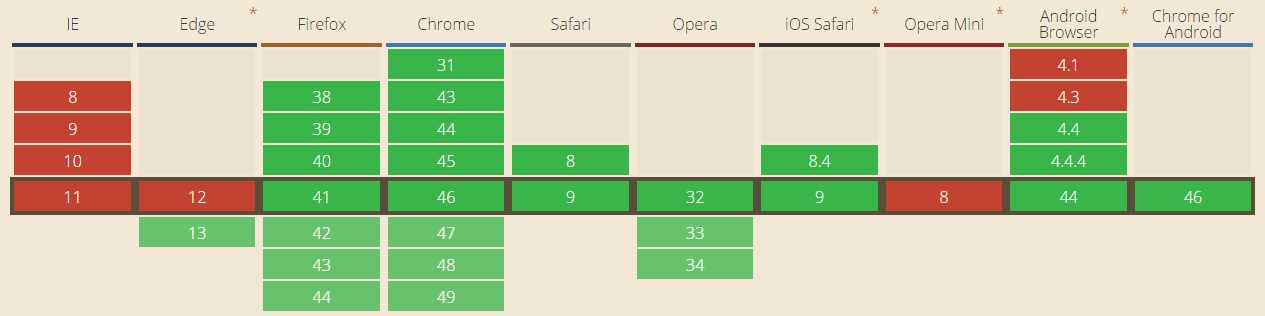
\includegraphics[width=\linewidth]{kapitel2/bilder/4-html-templates-browserunterstuetzung}
 \caption{Browserunterstützung des HTML Template Tags}
 \label{fig:bdhtmltt}
\end{figure}

\section{Shadow DOM}\label{shadow-dom}

Durch Kapselung ist es möglich, Details eines Objektes von anderen Teilen des Programms zu verstecken. Das Programm muss nur wissen, wie es auf die benötigten Funktionen zugreift, jedoch nicht, wie das Objekt die Funktionen intern umsetzt. Dieses Konzept ist in allen objektorientierten Programmiersprachen umgesetzt, jedoch nicht in der Webentwicklung. Beispielsweise kann das \ac{CSS} oder JavaScript, das für ein Element geschrieben ist, auch das \ac{CSS} oder JavaScript anderer Elemente beeinflussen. Je größer das Projekt wird, desto unübersichtlicher und komplexer wird es, zu gewährleisten, dass \ac{CSS} oder JavaScript sich nicht ungewollt auf andere Teile der Webseite auswirkt.

Diesem Problem widmet sich das sogenannte Shadow \ac{DOM}, welches ein Sub-\ac{DOM} unterhalb eines Elements darstellt und es ermöglicht, \ac{HTML} und \ac{CSS} in sich zu kapseln und zu verstecken. Als Kontrast zu Bezeichnung ``Shadow \ac{DOM}'' wird das reguläre \ac{DOM} des Hauptdokuments auch oft als ``Light \ac{DOM}'' bezeichnet. Das Shadow \ac{DOM} wird bereits in \ac{HTML}5 standardmäßig eingesetzt, wie beispielsweise im \texttt{\textless{}input\textgreater{}}-Tag. Beim Inspizieren des Elements mit Hilfe der Chrome Developer Tools (siehe Abbildung \ref{fig:itpelem}) wird deutlich, dass das \texttt{\textless{}input\textgreater{}}-Tag ein Shadow \ac{DOM} beinhaltet, welches das eingegebene Passwort kapselt. \cite[S. 109-126]{citeulike:13844975}

\begin{figure}[htbp]
 \centering
 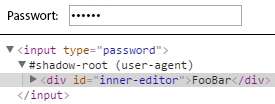
\includegraphics{kapitel2/bilder/3-shadow-dom-input-type-password}
 \caption{Passwort-Input-Element}
 \label{fig:itpelem}
\end{figure}


\subsection{Shadow DOM nach W3C}\label{shadow-dom-nach-w3c}

\begin{figure}[htbp]
 \centering
 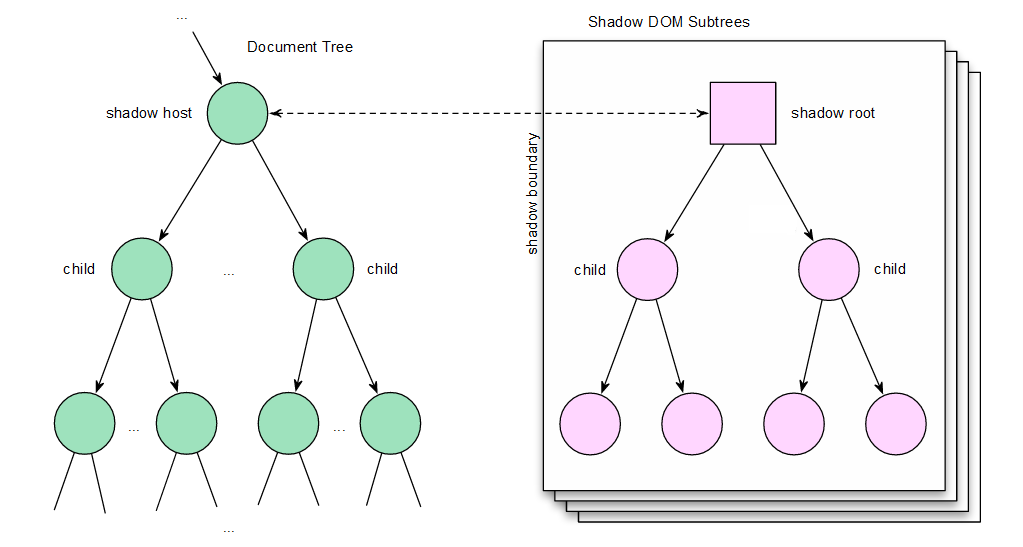
\includegraphics[width=\linewidth]{kapitel2/bilder/3-shadow-dom-shadow-boundary}
 \caption{Shadow \ac{DOM} und Shadow Boundary nach W3C}
 \label{fig:sdsbnw3c}
\end{figure}

Wie auf Abbildung \ref{fig:sdsbnw3c} zu sehen, liegt das Shadow \ac{DOM} dabei parallel zu dem \ac{DOM}-Knoten des beinhaltenden Elements. Ein Knoten im Document Tree (links abgebildet) wird als ``Shadow Host'' - ein Element, welches ein Shadow \ac{DOM} beinhaltet - markiert. Die gestrichelte Linie zeigt die Referenz zu der entsprechenden Shadow \ac{DOM} Wurzel, dem ``Shadow Root''. Die Referenz geht dabei durch die sogenannte ``Shadow Boundary'', welche es ermöglicht, den Shadow \ac{DOM}, und alles was dieser beinhaltet, zu kapseln \cite{citeulike:13851350}. Dies verhindert, dass externes \ac{CSS} oder JavaScript das interne Markup oder umgekehrt internes \ac{CSS} oder JavaScript den Light \ac{DOM} oder andere Shadow \ac{DOM}s ungewollt beeinflussen können. Ein Element kann auch mehrere Shadow \ac{DOM} Wurzeln referenzieren, allerdings wird nur die zuletzt hinzugefügte vom Browser gerendert, da dieser zum Rendern einen \ac{LIFO} Stack benutzt. Dabei wird der zuletzt hinzugefügte Shadow Tree ``Youngest Tree'' genannt, der jeweils zuvor hinzugefügte Shadow Tree wird ``Older Tree'' genannt. Das dynamische Hinzufügen von Shadow \ac{DOM}s ermöglicht es, die Inhalte der Webseite nach dem Rendern zu ändern.


\subsection{Content Projection}\label{content-projection}

Neben dem vom Shadow \ac{DOM} vorgegebenen \ac{HTML}, können auch Inhalte aus dem Light \ac{DOM} in den Shadow \ac{DOM} projiziert werden. Der Shadow \ac{DOM} nimmt dabei die zu projizierenden Inhalte und projiziert sie an der vorgegebenen Stelle im Shadow \ac{DOM}. Die Inhalte bleiben dabei an der ursprünglichen Stelle im \ac{DOM} stehen und werden nicht verschoben, gelöscht oder geändert. Der Shadow \ac{DOM} ermöglicht es somit eigenes, gekapseltes \ac{HTML} sowie dynamische Inhalte des Light \ac{DOM} anzuzeigen. Diese Projektion der Inhalte aus dem Light \ac{DOM} in den Shadow \ac{DOM} erfolgt mittels sogenannten ``Insertion Points''. Diese sind vom Entwickler definierte Stellen im Shadow \ac{DOM}, in welche der Inhalt projiziert wird. Es kann hierbei zwischen 2 Arten von Insertion Points unterschieden werden.

\subsection{Insertion Points}\label{insertion-points}

Um das zu präsentierende \ac{HTML} und den Inhalt zu trennen, wird ein \texttt{\textless{}template\textgreater{}}-Tag benutzt. Dieses beinhaltet das komplette Markup, das im Shadow \ac{DOM} stehen und nicht nach außen sichtbar sein oder von \ac{CSS} oder JavaScript von außen manipuliert werden soll. Um nun Inhalte aus dem Light \ac{DOM} in das \ac{DOM} des \texttt{\textless{}template\textgreater{}}-Tags zu projizieren, muss das \texttt{\textless{}template\textgreater{}}-Tag einen \texttt{\textless{}content\textgreater{}}-Tag beinhalten, in welchem die Inhalte von außen dargestellt werden sollen. Mittels \texttt{createShadowRoot()} wird das ausgewählte Element zu einem Shadow Host, also dem Shadow \ac{DOM} beinhaltendem Element gemacht. Der Inhalt des Templates wird geklont und dem Shadow Host angehängt. Das Shadow \ac{DOM} projiziert nun alle Inhalte des Shadow Roots in den \texttt{\textless{}content\textgreater{}}-Tag (siehe Listing \ref{tdueesd}) \cite{citeulike:13851404}.

\lstinputlisting[float,floatplacement=H,language=HTML,label=tdueesd,caption=Template-Definition und Erstellen eines Shadow \ac{DOM}s]{kapitel2/listings/3-1.html}

Im Light \ac{DOM} gerendert wird dabei nur der Text ``Inhalt'' des \texttt{\textless{}div\textgreater{}}-Tags mit der ID \texttt{shadow}, der Wrapper um das \texttt{\textless{}content\textgreater{}}-Tag wird nicht gerendert, da dieser im Shadow \ac{DOM} steht. Somit wurde eine Trennung des präsentierenden \ac{HTML} und dem Inhalt erreicht, die Präsentation erfolgt im Shadow \ac{DOM}, der Inhalt steht im Light \ac{DOM}. Werden nun mehrere \ac{HTML}-Elemente oder Knoten in den Shadow \ac{DOM} projiziert, werden diese ``Distributed Nodes'' genannt. Diese Distributed Nodes sind nicht wirklich im Shadow \ac{DOM}, sondern werden nur in diesem gerendert, was bedeutet, dass sie auch von außen gestylt werden können, mehr dazu im Abschnitt \ref{styling-mit-css}. Des Weiteren können auch nur bestimmte Elemente in das Shadow \ac{DOM} projiziert werden, ermöglicht wird dies mit dem Attribut \texttt{select=\dq selector\dq} des \texttt{\textless{}content\textgreater{}}-Tags. Dabei können sowohl Namen von Elementen, als auch \ac{CSS} Selektoren verwendet werden \cite{citeulike:13851402}. Der Inhalt des \texttt{\textless{}content\textgreater{}}-Tags kann mit JavaScript nicht traversiert werden, beispielsweise gibt \texttt{console.log(shadow.querySelector('content'));} \texttt{null} aus. Allerdings ist es erlaubt, die Distributed Nodes mittels \texttt{.getDistributedNodes()} auszugeben. Dies lässt darauf schließen, dass der Shadow \ac{DOM} nicht als Sicherheits-Feature angedacht ist, da die Inhalte nicht komplett isoliert sind.

\subsection{Shadow Insertion Points}\label{shadow-insertion-points}

Neben den \texttt{\textless{}content\textgreater{}}-Tags gibt es auch die \texttt{\textless{}shadow\textgreater{}}-Tags, welche Shadow Insertion Points genannt werden. Shadow Insertion Points sind ebenso wie Insertion Points Platzhalter, doch statt einem Platzhalter für den Inhalt eines Hosts, sind sie Platzhalter für Shadow \ac{DOM}s. Falls jedoch mehrere Shadow Insertion Points in einem Shadow \ac{DOM} sind, wird nur der erste berücksichtigt, die restlichen werden ignoriert. Wenn nun mehrere Shadow \ac{DOM}s projiziert werden sollen, muss im zuletzt hinzugefügten Shadow \ac{DOM} - dem ``Younger Tree'' - ein \texttt{\textless{}shadow\textgreater{}}-Tag stehen, dieser rendert den zuvor hinzugefügten Shadow \ac{DOM} - den ``Older Tree''. Somit wird eine Schachtelung mehrerer Shadow \ac{DOM}s ermöglicht \cite{citeulike:13851421}.

\subsection{Styling mit CSS}\label{styling-mit-css}

Eines der Hauptfeatures des Shadow \ac{DOM}s ist die Shadow Boundary, welche Kapselung von Stylesheets standardmäßig mit sich bringt. Sie gewährleistet, dass Style-Regeln des Light \ac{DOM} nicht den Shadow \ac{DOM} beeinflussen und umgekehrt \cite{citeulike:13851334}. Dies gilt jedoch nur für die Präsentation des Inhalts, nicht für den Inhalt selbst. Nachfolgend wird auf die wichtigsten Selektoren für das Styling eingegangen.

\begin{description}
  \item[:host] Das Host-Element des Shadow \ac{DOM}s kann mittels dem Pseudoselektor \texttt{:host} angesprochen werden. Dabei kann dem Selektor optional auch ein Selektor mit übergeben werden wie beispielsweise mit \texttt{:host(.myHostElement)}. Mit diesem Selektor ist es möglich, nur Hosts, welche diese Klasse haben, anzusprechen. Zu beachten ist, dass das Host-Element von außen gestylt werden kann, also die Regeln des \texttt{:host}-Selektors überschreiben kann. Des Weiteren funktioniert der \texttt{:host}-Selektor nur im Kontext eines Shadow \ac{DOM}s, man kann ihn also nicht außerhalb benutzen. Besonders wichtig ist dieser Selektor, wenn auf die Aktivität der Benutzer reagiert werden muss. So kann innerhalb des Shadow \ac{DOM}s angegeben werden, wie das Host Element beispielsweise beim Hover mit der Maus auszusehen hat.
  \item[:host-context()] Je nach Kontext eines Elements kann es vorkommen, dass Elemente unterschiedlich dargestellt werden müssen. Das wohl am häufigsten auftretende Beispiel hierfür ist das Theming. Themes ermöglichen es, Webseiteninhalte auf unterschiedliche Arten darzustellen. Oftmals bietet eine Webseite oder eine Applikation mehrere Themes für die Benutzer an, zwischen welchen sie wechseln können. Mit dem \texttt{:host-context()}-Selektor wird es möglich, ein Host-Element je nach Klasse des übergeordneten Elements - dem Parent-Element - zu definieren. Hat ein Host-Element mehrere Style-Definitionen, so werden diese nach der Klasse des Parent-Elements getriggert. Soll eine Style-Definition beispielsweise nur angewendet werden, wenn das umschließende Element die Klasse \texttt{theme-1} hat, so kann das mit \texttt{:host-context(.theme-1)} erreicht werden.
\end{description}


\subsection{Styling des Shadow DOM von außerhalb}\label{styling-des-shadow-dom-von-ausserhalb}

Trotz der Kapselung von Shadow \ac{DOM}s ist es mit speziellen Selektoren möglich, die Shadow Boundary zu durchbrechen. So können Style-Regeln für Shadow Hosts oder in ihm enthaltene Elemente vom Elterndokument definiert werden \cite{citeulike:13883067}.

\begin{description}
  \item[::shadow] Falls ein Element nun einen Shadow Tree beinhalten sollte, so kann dieses mit der entsprechenden Klasse oder ID sowie dem \texttt{::shadow}-Selektor angesprochen werden. Jedoch können mit diesem Selektor keine allgemeingültigen Regeln erstellt werden. Stattdessen muss stets ein in dem Shadow Tree enthaltener Elementname angesprochen werden. Nimmt man sich nun die Content Insertion Points zur Hilfe, so ist es dennoch möglich, Regeln für mehrere unterschiedliche Elemente zu definieren. Die Selektor-Kombination \texttt{\#my-element::shadow\ content} Spricht nun alle \texttt{\textless{}content\textgreater{}}-Tags an, welche im Shadow Tree des Elements \texttt{\#my-element} vorhanden sind. Da in diesen \texttt{\textless{}content\textgreater{}}-Tag wiederum die Inhalte hineinprojiziert werden, werden die Regeln für die projizierten Elemente angewendet. Sollten nun noch weitere Shadow \ac{DOM}s in diesem Element geschachtelt sein, so werden die Regeln jedoch nicht für diese angewandt, sondern nur für das direkt folgende Kind des Elements \texttt{\#my-element}.
  \item[\textgreater{}\textgreater{}\textgreater{}] Dieser Kombinator ist ähnlich dem \texttt{::shadow}-Selektor. Er bricht jedoch durch sämtliche Shadow Boundaries und wendet die Regeln auf alle gefundenen Elemente an. Dies gilt - im Gegensatz zum \texttt{::shadow}-Selektor - auch für geschachtelte Shadow Trees. Mit dem Selektor \texttt{my-element\ \textgreater{}\textgreater{}\textgreater{}\ span} werden also alle im Element \texttt{\textless{}my-element\textgreater{}} sowie in dessen geschachtelten Shadow Trees enthaltenen \texttt{\textless{}span\textgreater{}}-Elemente angesprochen.
  \item[::slotted] Die Kombination \texttt{\#my-element::shadow\ content} zeigt die Möglichkeit, wie die Inhalte eine Shadow \ac{DOM}s von außen gestylt werden können. Sollen jene in den Content Insertion Points enthaltenen ELemente jedoch von innerhalb gestylt werden, so ist dies mit dem \texttt{::slotted}-Selektor möglich. Ist innerhalb eines Elements die Regel \texttt{::slotted\ p} definiert, so werden alle in den Shadow \ac{DOM} projizierten \texttt{\textless{}p\textgreater{}}-Tags angesprochen.
\end{description}


\subsection{CSS-Variablen}\label{css-variablen}

Die oben gezeigten Selektoren und Kombinatoren eignen sich hervorragend um die Shadow Boundary zu durchdringen und eigene Styles den Elementen aufzuzwingen. Jedoch sprengen sie das Prinzip der Kapselung, das man mit Web Components zu gewinnen versucht. Dennoch haben sie ihre Existenzberechtigung. Sie ermöglichen es den Entwicklern, fremde Components sowie native \ac{HTML}-Elemente, die einen Shadow \ac{DOM} benutzen, wie z.B. \texttt{\textless{}video\textgreater{}} oder \texttt{\textless{}input\textgreater{}}-Elemente, zu stylen. Allerdings sollte bei ihrer Anwendung äußerst vorsichtig gearbeitet werden, besonders da sie schnell missbraucht werden können.

Ein Ansatz zur Lösung dieser Problematik sind \ac{CSS}-Variablen. Mit ihnen können Elemente in ihrem Shadow \ac{DOM} Variablen für die inneren Styles bereit halten, welche von außerhalb des Shadow \ac{DOM}s instanziiert werden können. Dadurch ist es möglich, das innere Styling eines Elements nach außen zu reichen. Statt die Barriere nun zu durchbrechen, können Elemente miteinander kommunizieren. Es wird somit eine Style-Schnittstelle geschaffen \cite{citeulike:13883381}. Ein Element \texttt{my-element} kann nun in dessen Shadow \ac{DOM} beispielsweise die Schriftfarbe mit \texttt{color} definieren. Doch statt einem Wert wird nun der Name der nach außen sichtbaren Variablen angegeben. Die Syntax hierfür lautet \texttt{var(-\/-varable-name,\ red)}, wobei \texttt{red} hier der Standardwert ist, falls die Variable \texttt{-\/-variable-name} von außen nicht gesetzt wird. Nachdem die Variable definiert wurde, kann sie von außerhalb des Shadow \ac{DOM} mittels der Regel \texttt{\#my-shadow-host\ \{\ -\/-varable-name:\ blue;\ \}} überschrieben werden.


\newpage
\subsection{Beispiel eines Shadow DOMs mit Template und CSS}\label{beispiel-eines-shadow-doms-mit-template-und-css}

Listing \ref{biesdmtucss} zeigt eine exemplarische Implementierung eines Shadow \ac{DOM}s, welcher gekapseltes \ac{CSS} und JavaScript beinhaltet.

\lstinputlisting[language=HTML,label=biesdmtucss,caption=Beispielimplementierung eines Shadow \ac{DOM}s mit Template und \ac{CSS}]{kapitel2/listings/3-2.html}

Das obige Beispiel wird vom Browser, wie in Abbildung \ref{fig:shadowdombeispiel} dargestellt, gerendert.

\begin{figure}[htbp]
 \centering
 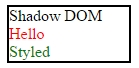
\includegraphics{kapitel2/bilder/3-shadow-dom-beispiel}
 \caption{Shadow DOM Beispiel}
 \label{fig:shadowdombeispiel}
\end{figure}

Anhand des gerenderten Outputs werden einige Dinge deutlich. Mit der Angabe des \texttt{select}-Attributs, werden im \texttt{\textless{}content\textgreater{}}-Tag nur die \texttt{\textless{}div\textgreater{}}-Tags mit der ID \texttt{hello} aus dem Shadow Root, welcher per \texttt{var\ root\ =\ document.querySelector('\#hello').createShadowRoot()} erzeugt wird, gerendert. Der Paragraph mit der ID \texttt{hidden} wird hingegen nicht gerendert, da er nicht im \texttt{select} mit inbegriffen ist. Die \ac{CSS}-Regel \texttt{.content\ \{\ background-color:\ khaki;\ \}} des Eltern-\ac{HTML}-Dokuments greift nicht, da die Styles des Shadow Roots durch die Shadow Boundary gekapselt werden. Die \ac{CSS} Regel \texttt{.styled\ \{\ color:\ green;\ \}} greift allerdings, da das \texttt{\textless{}div\textgreater{}}-Element mit der Klasse \texttt{styled} aus dem Light \ac{DOM} in den Shadow \ac{DOM} projiziert wird. Außerdem können innerhalb des Templates CSS-Regeln für die beinhaltenden Elemente definiert werden, somit wird das \texttt{\textless{}div\textgreater{}}-Element ohne eine zugehörige Klasse mit der Regel \texttt{.content\ \{\ color:\ red;\ \}} auch dementsprechend in Rot gerendert.


\subsection{Browserunterstützung}\label{shadow-dom-browserunterstuetzung}

Der Shadow \ac{DOM} ist noch nicht vom \ac{W3C} standardisiert, sondern befindet sich noch im Status eines ``Working Draft'' \cite{citeulike:13879687}. Er wird deshalb bisher nur von Google Chrome ab Version 43 und Opera ab Version 33 nativ unterstützt (siehe Abbildung \ref{fig:shadowdombrowser}) \cite{citeulike:13883407}.

\begin{figure}[htbp]
 \centering
 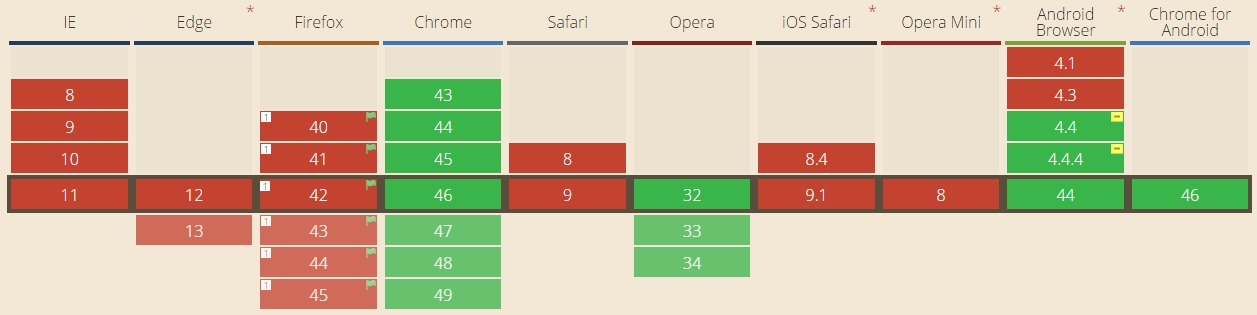
\includegraphics[width=\linewidth]{kapitel2/bilder/3-shadow-dom-browserunterstuetzung}
 \caption{Browserunterstützung des Shadow DOMs}
 \label{fig:shadowdombrowser}
\end{figure}

\section{HTML Imports}\label{html-imports}

Bisher erlauben es praktisch alle Plattformen, Codeteile zu importieren und zu verwenden, nur nicht das Web bzw. \ac{HTML}. Das heutige \ac{HTML} ermöglicht es externe Stylesheets, JavaScript Dateien, Bilder etc. in ein \ac{HTML} Dokument zu importieren, \ac{HTML}-Dateien selbst können jedoch nicht importiert werden. Auch ist es nicht möglich, alle benötigten Dateien in einer Ressource zu bündeln und als einzige Abhängigkeit zu importieren. \ac{HTML} Imports versuchen eben dieses Problem zu lösen. So soll es möglich sein, \ac{HTML}-Dateien und wiederum \ac{HTML}-Dateien in \ac{HTML}-Dateien zu importieren. So können auch verschiedene benötigte Dateien in einer \ac{HTML}-Datei gesammelt und mit nur einem Import in die Seite eingebunden werden. Doppelte Abhängigkeiten sollen dadurch automatisch aufgelöst werden, sodass Dateien, die mehrmals eingebunden werden sollten, automatisch effektiv nur einmal heruntergeladen werden.


\subsection{HTML-Dateien importieren}\label{html-dateien-importieren}

Imports von \ac{HTML}-Dateien werden, wie andere Imports auch, per \texttt{\textless{}link\textgreater{}}-Tag deklariert. Neu ist jedoch der Wert des \texttt{rel}-Attributes, welches auf \texttt{import} gesetzt wird \cite[S. 139-147]{citeulike:13844975}. So kann beispielsweise das Bootstrap-Frame\-work statt wie bisher mit mehreren Imports mit nur einem Import eingebunden werden. Bisher könnte die Einbindung unter Berücksichtigung der Abhängigkeiten wie in Listing \ref{evbohtmli} aussehen.

\lstinputlisting[language=HTML,label=evbohtmli,caption=Einbindung von Bootstrap ohne \ac{HTML} Imports]{kapitel2/listings/5-1.html}

Stattdessen kann dieses Markup nun in ein einziges \ac{HTML} Dokument, welches alle Abhängigkeiten verwaltet, geschrieben werden. Dieses wird dann mit einem einzigen Import \texttt{\textless{}link\ rel=\dq import\dq\ href=\dq bootstrap.html\dq\textgreater{}} in das eigene \ac{HTML} Dokument importiert.

Es ist jedoch zu beachten, dass \ac{HTML} Imports nur auf Ressourcen der gleichen Quelle, also dem gleichen Host, respektive der gleichen Domain zugreifen können. Imports von \ac{HTML}-Dateien von verschiedenen Quellen stellen eine Sicherheitslücke dar, da Webbrowser die \ac{SOP} verfolgen.

\begin{quote}
The same-origin policy restricts how a document or script loaded from one origin can interact with a resource from another origin. It is a critical security mechanism for isolating potentially malicious documents. \cite{citeulike:13853253}
\end{quote}

Sollte das jedoch dennoch erlaubt werden, so muss das \ac{CORS} für die entsprechende Domain auf dem Server aktiviert werden.

\begin{quote}
These restrictions prevent a client-side Web application running from one origin from obtaining data retrieved from another origin, and also limit unsafe \ac{HTTP} requests that can be automatically launched toward destinations that differ from the running application's origin. \cite{citeulike:13853643}
\end{quote}


\subsection{Auf importierte Inhalte zugreifen}\label{html-imports-verwenden}

Importierte \ac{HTML}-Dateien werden nicht nur in das Dokument eingefügt, sondern vom Parser verarbeitet, das bedeutet, dass mit JavaScript auf das \ac{DOM} des Imports zugegriffen werden kann. Wenn sie vom Parser verarbeitet worden sind, sind sie zwar verfügbar, allerdings werden die Inhalte nicht angezeigt bis sie mittels JavaScript in das \ac{DOM} eingefügt werden. Ihre enthaltenen Scripte werden also ausgeführt, Styles und \ac{HTML}-Knoten werden jedoch ignoriert. Um nun die Inhalte eines Imports auf der Seite einzubinden, muss auf die \texttt{.import} Eigenschaft des \texttt{\textless{}link\textgreater{}}-Tags mit dem Import zugegriffen werden \texttt{var\ content\ =\ document.querySelector('link{[}rel=\dq import\dq{]}').import;}. Nun kann auf das \ac{DOM} des Imports zugegriffen werden. So kann ein enthaltenes Element mit der Klasse \texttt{element} mit \texttt{var\ el\ =\ content.querySelector('.element');} geklont und anschließend durch \texttt{document.body.appendChild(el.cloneNode(true));} in das eigene \ac{DOM} eingefügt werden. Falls es jedoch mehrere Imports geben sollte, können den Imports IDs zugewiesen werden, anhand derer die Imports voneinander unterschieden werden können (siehe Listing \ref{euvvhtmli}) \cite{citeulike:13853724}.

\lstinputlisting[language=HTML,label=euvvhtmli,caption=Einbinden und Verwenden von \ac{HTML} Imports]{kapitel2/listings/5-2.html}


\subsection{Abhängigkeiten verwalten}\label{abhuxe4ngigkeiten-verwalten}

Jedoch kann es vorkommen, dass mehrere eingebundenen Bibliotheken die gleichen Abhängigkeiten haben und diese verwaltet werden müssen. Sollte dies nicht sorgfältig gemacht werden, können unerwartete Fehler auftreten, die mitunter nur schwer zu lokalisieren sind. \ac{HTML} Imports verwalten Abhängigkeiten automatisch. Um das zu erreichen, werden die Abhängigkeiten gebündelt und in eine zu importierende \ac{HTML}-Datei geschrieben. Haben mehrere Imports die gleichen Abhängigkeiten (siehe Listing \ref{ahvmhtmli}), werden diese vom Browser erkannt und nur einmal heruntergeladen. Mehrfachdownloads und Konflikte der Abhängigkeiten werden so verhindert \cite{citeulike:13853700}.

\lstinputlisting[language=HTML,label=ahvmhtmli,caption=Abhängigkeitsverwaltung mit \ac{HTML} Imports]{kapitel2/listings/5-3.html}

Selbst wenn die jQuery-Library in mehreren Dateien eingebunden wird, wird hier sie dennoch nur einmal übertragen. Wenn nun fremde \ac{HTML}-Dateien eingebunden werden, muss auch nicht auf die Reihenfolge der Imports geachtet werden, da diese selbst ihre Abhängigkeiten beinhalten.


\subsection{Sub-Imports}\label{sub-imports}

Das obige Beispiel zeigt, dass \ac{HTML} Imports selbst wiederum auch \ac{HTML} Imports beinhalten können. Diese Imports werden Sub-Imports genannt und ermöglichen einen einfachen Austausch oder eine Erweiterungen von Abhängigkeiten innerhalb einer Komponente. Wenn eine Komponente A eine Abhängigkeit von einer Komponenten B hat und eine neue Version von Komponente B verfügbar ist, kann dies einfach in dem Import des Sub-Imports angepasst werden ohne den Import in der Eltern-\ac{HTML}-Datei anpassen zu müssen \cite{citeulike:13853647}.


\subsection{Performance}\label{html-import-performance}

Ein signifikantes Problem der \ac{HTML} Imports ist die Performance, welche bei komplexen Anwendungen schnell abfallen kann. Werden auf einer Seite mehrere Imports eingebunden, die selbst wiederum Imports beinhalten können, so steigt die Anzahl an Requests an den Server schnell exponentiell an, was die Webseite stark verlangsamen kann. Auch das Vorkommen von doppelten Abhängigkeiten kann die Anzahl an Requests in die Höhe treiben, doch da Browser die Abhängigkeiten nativ schon selbst de-duplizieren, kann dieses Problem in diesem Zusammenhang ignoriert werden \cite{citeulike:13853714}.

Dennoch sind viele Einzel-Requests ein gewünschtes Verhalten von Web Components, da sie bereits mit Blick auf Version 2 des \ac{HTTP}-Protokolls entwickelt wurden. In diesem können mehrere Requests in einer \ac{TCP}-Verbindung übertragen werden. Des Weiteren kann der Client die Priorität der angeforderten Dateien bestimmen, um Dateien mit einer hohen Priorität vor Dateien mit niedrigerer Priorität zu erhalten. Ebenso wird mit einer neuen Header-Kompression die zu übertragende Datenmenge verkleinert. Neu sind außerdem die sogenannten ``Server Pushes'', welche es dem Server ermöglichen, Nachrichten an den Client zu schicken, ohne dass dieser sie anfordern muss.

Voraussetzung hierfür ist jedoch die Unterstützung des neuen Protokolls seitens des Browsers. Bis auf den Internet Explorer und Safari unterstützen jedoch alle Browser \ac{HTTP}/2 schon ab frühen Versionen, allerdings nur bei mittels \ac{TLS} verschlüsselten Webseiten \cite{citeulike:13879562}. Der Anteil der über \ac{HTTP}/2 ausgelieferten Webseiten liegt momentan bei circa 3\% \cite{citeulike:13879575}.


\subsection{Asynchrones Laden von Imports}\label{asynchrones-laden-von-imports}

Das Rendern der Seite kann unter Umständen sehr lange dauern, da das in den Imports enthaltene JavaScript das Rendern blockiert. Um das zu verhindern und alle Dateien möglichst schnell laden zu können, ist ein \texttt{async}-Attribut vorgesehen. Dieses funktioniert jedoch nur, wenn als Protokoll \ac{HTTP}/2 gewählt wird. Das Attribut ermöglicht es, dass mehrere Dateien asynchron geladen werden können. In den Imports enthaltenes JavaScript blockiert somit nicht das Rendern von bereits geladenem \ac{HTML} Code. Falls \ac{HTTP}/2 nicht vorhanden sein sollte, kann alternativ das \texttt{defer}-Attribut gewählt werden, wodurch das JavaScipt erst nach vollständigem Parsen des \ac{HTML} ausgeführt wird. Eine weitere Methode ist das Laden der Imports am Ende der Seite. Somit wird sichergestellt, dass die Scripte erst ausgeführt werden, wenn die Seite geladen und gerendert wurde.


\subsection{Anwendungen}\label{anwendungen}

Besonders einfach machen \ac{HTML} Imports das Einbinden ganzer Web Applikationen mit \ac{HTML}/JavaScript/\ac{CSS}. Diese können in eine Datei geschrieben, ihre Abhängigkeiten definieren und von anderen importiert werden. Dies macht es sehr einfach, den Code zu organisieren. So können etwa einzelne Abschnitte von Anwendungen oder Code in einzelne Dateien ausgelagert werden, was Web Applikationen modular, austauschbar und wiederverwendbar macht. Falls nun ein oder mehrere Custom Elements in einem \ac{HTML} Import enthalten sind, so werden dessen Interface und Definitionen automatisch gekapselt. Auch wird die Abhängigkeitsverwaltung in Betracht auf die Performance stark verbessert, da der Browser nicht eine große JavaScript-Library, sondern einzelne kleinere JavaScript-Abschnitte parsen und ausführen muss. Diese werden durch die \ac{HTML} Imports parallel geparst, was mit einem enormen Performance-Schub einher geht \cite{citeulike:13853647}.


\subsection{Browserunterstützung}\label{browserunterstuxfctzung}

\ac{HTML} Imports sind noch nicht vom \ac{W3C} standardisiert, sondern befinden sich noch im Status eines ``Working Draft'' \cite{citeulike:13853711}. Sie werden deshalb bisher nur von Google Chrome ab Version 43 und Opera ab Version 33 nativ unterstützt (siehe Abbildung \ref{fig:bdhtmli}). Seitens Mozilla und dessen Browser Firefox wird es für \ac{HTML} Imports auch keine Unterstützung geben, da ihrer Meinung nach der Bedarf an \ac{HTML} Imports nach der Einführung von ECMAScript 6 Modules nicht mehr existiert und da Abhängigkeiten schon mit Tools wie Vulcanize aufgelöst werden können \cite{citeulike:13881144}. Auf Details zu ECMAScript 6 Modules wird an dieser Stelle nicht eingegangen, da diese den Umfang dieser Arbeit überschreiten.

\begin{figure}[htbp]
 \centering
 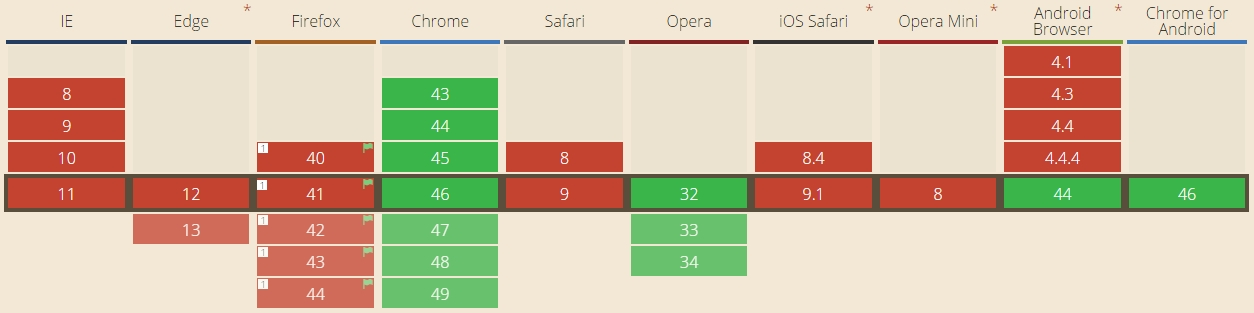
\includegraphics[width=\linewidth]{kapitel2/bilder/5-html-imports-browserunterstuetzung}
 \caption{Browserunterstützung der HTML Imports}
 \label{fig:bdhtmli}
\end{figure}


\section{Polyfills}\label{polyfills-mit-webcomponents.js}

In den Abschnitten \ref{custom-elements} bis \ref{html-imports} wurde gezeigt, wie die Web-Components-Technologien funktionieren und ob diese bereits in allen Browsern unterstützt werden. In diesem Abschnitt wird genauer darauf eingegangen was Polyfills sind. Ebenso wird auf deren Performance eingegangen und wie sie die Browserunterstützung der Web-Components-Technologien verbessern.


\subsection{Native Browserunterstützung von Web Components}\label{native-browserunterstuxfctzung-von-web-components}

In den einzelnen Unterkapiteln zu den Technologien wurde jeweils kurz gezeigt, ob diese von den Browsern unterstützt wird oder nicht. Es wurde deutlich, dass Chrome und Opera bisher die einzigen Vorreiter sind. Bis auf \ac{HTML} Templates, welche von allen modernen Browsern unterstützt werden, unterstützen sie als einzige alle Technologien. \cite{citeulike:13914379}

\begin{description}
  \item[Chrome] Hat alle Spezifikationen der Web-Component-Standards ab Version 43 komplett implementiert.
  \item[Firefox] Unterstützt nativ \ac{HTML} Templates. Custom Elements und Shadow \ac{DOM} sind zwar implementiert, müssen aber über das Flag \texttt{dom.webcomponents.enabled} manuell in den Entwicklereinstellungen aktiviert werden. \ac{HTML} Imports werden, wie in Kapitel \ref{html-imports} erwähnt, bis auf Weiteres nicht unterstützt.
  \item[Safari] \ac{HTML} Templates werden ab Version 8 unterstützt, Custom Elements und Shadow \ac{DOM} befinden sich in der Entwicklung (Stand Januar 2016), \ac{HTML} Imports werden jedoch nicht unterstützt.
  \item[Internet Explorer] Als einziger Browser unterstützt der Internet Explorer keine der Web-Components-Technologien. Die Unterstützung wird -- auf Grund der Einstellung der Entwicklung und des Wechsels zu Microsoft Edge -- auch nicht nachträglich implementiert werden.
  \item[Microsoft Edge] Templates werden ab Version 13 unterstützt, über die Entwicklung der restlichen Technologien kann allerdings abgestimmt werden \cite{citeulike:13914237}.
  \item[Mobile Browser] Alle Technologien werden bisher nur auf Android in den Browsern Chrome für Android, Opera und Android Browser unterstützt.
\end{description}

Die Browserunterstützung der Technologien der Web Components ist momentan also noch verhalten. Das bedeutet jedoch nicht, dass sie noch nicht verwendet werden können. Mittels JavaScript besteht die Möglichkeit, die Technologien den Browsern beizubringen, welche sie nicht unterstützen. Ein solches JavaScript wird ``Polyfill'' genannt.


\subsection{Polyfill webcomponents.js}\label{polyfill-webcomponents.js}

\begin{quote}
A polyfill, or polyfiller, is a piece of code (or plugin) that provides the technology that you, the developer, expect the browser to provide natively. \cite{citeulike:13914241}
\end{quote}

Mit Hilfe von Polyfills können die Technologie-Lücken der Browser also auf mehrere, unterschiedliche Arten (``Poly'') gefüllt (``fill'') werden \cite{citeulike:13914234}. Eine Sammlung an Polyfills Technologien der Web Components bildet das JavaScript webcomponents.js. Es wurde von Google im Rahmen von Polymer entwickelt und hat eine dermaßen weite Verbreitung erfahren, dass es auszugliedern wurde. Somit kann es auch unabhängig von der Benutzung von Polymer eingesetzt werden \cite{citeulike:13914239}.


\subsection{Browserunterstützung}\label{polyfills-browserunterstuetzung}

Mit dem Einsatz der webcomponents.js Polyfills werden die Web Components auch auf den Internet Explorer, Firefox sowie Safari portiert. Eine detaillierte Matrix der Browserunterstützung der Web Components mit Einsatz der Polyfills ist in Abbildung \ref{fig:bdwctmwcjs} \cite{citeulike:13914238} dargestellt.

\begin{figure}[htbp]
 \centering
 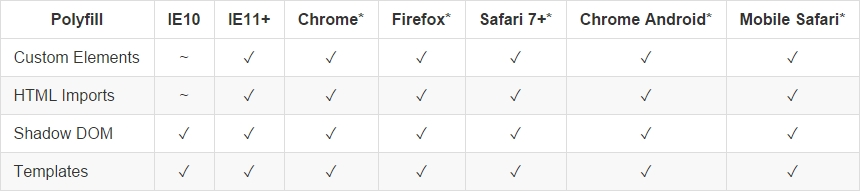
\includegraphics[width=\linewidth]{kapitel2/bilder/6-webcomponentsjs-browserunterstuetzung}
 \caption{Browserunterstützung der Web Components Technologien mit webcomponents.js}
 \label{fig:bdwctmwcjs}
\end{figure}

Jedoch werden die Technologien der Web Components auch mit Einsatzes der Polyfills nur von den aktuelleren Versionen des jeweiligen Browsers unterstützt. Darunter fallen jedoch weiterhin nicht ältere Browser, wie beispielsweise der Internet Explorer in Version 8 und 9. Des Weiteren werden einige Technologien auf Grund der Komplexität nicht komplett simuliert. Hier muss bei einigen Technologien auf folgende Punkte geachtet werden.

\begin{description}
  \item[Custom Elements] Die \ac{CSS}-Pseudoklasse \texttt{:unresolved} wird nicht unterstützt.
  \item[Shadow \ac{DOM}] Das Shadow \ac{DOM} kann auf Grund der Kapselung nicht komplett künstlich simuliert werden, dennoch versucht das webcomponents.js Polyfill einige der Features zu simulieren. So sprechen definierte \ac{CSS}-Regeln alle Elemente in einem künstlichen Shadow Root an -- als würde man den \texttt{\textgreater{}\textgreater{}\textgreater{}} Selektor benutzen -- auch die \texttt{::shadow} und \texttt{::content} Pseudoelemente verhalten sich so.
  \item[\ac{HTML} Templates] Templates, welche mit einem Polyfill erzeugt werden, sind nicht unsichtbar für den Browser, ihre enthaltenen Ressourcen werden also schon beim initialen Laden der Seite heruntergeladen.
  \item[\ac{HTML} Imports] Die zu importierenden \ac{HTML}-Dateien werden mit einem \ac{XHR}, und somit asynchron heruntergeladen, selbst wenn das \texttt{async}-Attribut (siehe Abschnitt \ref{asynchrones-laden-von-imports}) nicht gesetzt ist.
\end{description}


\subsection{Performance}\label{performance}

Das webcomponents.js-JavaScript \cite{citeulike:13914238} bringt mit seiner Größe von 116 KB einen großen Umfang mit, was sich negativ auf die Ladezeiten der Webseite auswirkt. Des Weiteren müssen die von den Browsern nicht unterstützten und ignorierten \ac{CSS}-Regeln -- wie \texttt{::shadow} oder \texttt{::slotted} -- mit Regular Expressions nachgebaut werden, was momentan 40 Stück sind. Das macht die Polyfills extrem komplex und träge. Die Funktionen zum Traversieren des \ac{DOM}s müssen angepasst werden, damit nur die richtigen Elemente angezeigt werden und eine Shadow Boundary simuliert wird. Diese werden mit 42 Wrappern umgesetzt, was wie die Regular Expressions zur Simulation der \ac{CSS}-Regeln sehr aufwändig ist. Allerdings können einige Funktionen wie \texttt{window.document} schlichtweg nicht überschrieben werden. Im Allgemeinen wird die \ac{DOM}-\ac{API} stark verlangsamt, wodurch die Performance -- speziell auf mobilen Geräten -- drastisch sinkt und mitunter nicht tolerierbar ist \cite{citeulike:13886251}.


\subsection{\texorpdfstring{Request-Minimierung mit ``Vulcanize''}{Request-Minimierung mit Vulcanize}}\label{request-minimierung-mit-vulcanize}

Webseiten können viele verschiedene, modular aufgebaute JavaScript-Dateien, Stylesheets, etc. beinhalten, welche die Anzahl an Requests erhöhen. Um die Anzahl an Requests zu verringern gibt es in der Webentwicklung bereits mehrere verschiedene Hilfsmittel. So werden die einzelnen Stylesheets oder auch JavaScript Dateien zu einer einzigen Datei konkateniert, sodass für das komplette Styling und JavaScript jeweils eine große Datei entsteht, welche nur einen Request an den Server benötigen. Zusätzlich kann sie anschließend noch minifiziert werden, um ihre Größe zu verringern und die Ladezeiten zu verkürzen. Selbiges Prinzip kann auch auf die \ac{HTML} Imports angewendet werden. Google stellt hierfür das Tool Vulcanize \cite{citeulike:13879681} bereit, welches serverseitig ermöglicht, einzelne kleine Web Components in einer einzigen, großen Web Component zusammenzufassen. Benannt nach der Vulkanisation, werden metaphorisch die einzelnen Elemente in ein beständigere Materialien umgewandelt. Vulcanize reduziert dabei eine \ac{HTML}-Datei und ihre zu importierenden \ac{HTML}-Dateien in eine einzige Datei. Somit werden die unterschiedlichen Requests in nur einem einzigen gebündelt und die Ladezeiten sowie die benötigte Bandbreite minimiert.


\section{Implementierung einer Komponente mit den nativen Web-Component-APIs}\label{implementierung-einer-komponente-mit-den-nativen-web-component-apis}

Anhand der vorhergehenden Abschnitte wird in diesem Abschnitt die Implementierung der Web Komponente \texttt{\textless{}custom-element\textgreater{}} mit den nativen \ac{HTML} APIs erläutert. Diese soll dabei das Markup in einem Shadow \ac{DOM} kapseln und den übergebenen Inhalt darstellen. Des Weiteren soll dessen Farbe über das Attribut \texttt{theme} optional konfiguriert werden können. Die gerenderte Komponente wird in Abbildung \ref{fig:gwkmnapis} dargestellt.

\begin{figure}[htbp]
 \centering
 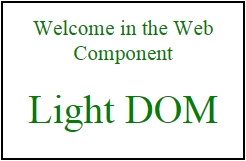
\includegraphics[width=5cm,keepaspectratio]{kapitel2/bilder/7-beispiel}
 \caption{Gerenderte Web Komponente mit nativen APIs}
 \label{fig:gwkmnapis}
\end{figure}


\subsection{Custom Element mit Eigenschaften und Funktionen definieren}\label{custom-element-mit-eigenschaften-und-funktionen-definieren}

Um ein neues Custom Element zu registrieren, wird zunächst ein \texttt{\ac{HTML}Element} Prototyp \texttt{CustomElementProto} mittels \texttt{Object.create(\ac{HTML}Element.prototype)} erstellt. Dieser wird anschließend um die Eigenschaft \texttt{theme} und dessen Standardwert \texttt{style1} erweitert, welches das deklarativ konfigurierbare
Attribut \texttt{theme} abbildet. Nun können die Lifecycle-Callback-Funktionen \texttt{createdCallback} und \texttt{attributeChangedCallback} der Komponente definiert werden (siehe Listing \ref{cemeufd}).

\lstinputlisting[language=JavaScript,label=cemeufd,caption=Custom Element mit Eigenschaften und Funktionen definieren]{kapitel2/listings/7-1.js}

Die \texttt{createdCallback}-Funktion soll zunächst prüfen ob das Attribut \texttt{theme} beim Verwenden des
\texttt{\textless{}custom-element\textgreater{}}-Tags verwendet und ein entsprechender Wert gesetzt wurde und übergibt dieses der Hilfsfunktion \texttt{setTheme}. Wird das Attribut nicht gesetzt, wird der Standardwert \texttt{style1} übergeben. Falls das \texttt{style}-Attribut von Außen geändert wird, soll die \texttt{attributeChangedCallback} Funktion gewährleisten, dass die Änderung auch von der Komponente übernommen wird, indem sie das Attribut der Hilfsfunktion \texttt{setTheme} übergibt. Um das Setzen und Ändern des \texttt{theme}-Attributs zu implementieren wird zuletzt die Hilfsfunktion \texttt{setTheme} für den Prototyp definiert (siehe Listing \ref{hsetthemed}).

\lstinputlisting[language=JavaScript,label=hsetthemed,caption=HilfsFunktion \texttt{setTheme} definieren]{kapitel2/listings/7-2.js}

Diese setzt den übergebenen Parameter, das \texttt{theme}-Attribut, als Klasse auf den umschließenden Wrapper \texttt{.outer}, welche dabei den zu verwendenden Style der Komponente bestimmt. Da der Prototyp nun alle erforderlichen Eigenschaften besitzt, kann er mit \texttt{document.registerElement(\dq custom-element\dq,\ \{\ prototype:\ CustomElementProto\ \});} als \ac{HTML}-Tag \texttt{custom-element} in dem importierenden Dokument verfügbar gemacht werden.


\subsection{Template erstellen und Styles definieren}\label{template-erstellen-und-styles-definieren}

Bisher ist das Custom Element zwar funktional, bietet aber noch kein gekapseltes Markup. Hierfür wird ein Template mit der ID \texttt{myElementTemplate} angelegt (siehe Listing \ref{teusd}), welches die für die Komponente notwendige \ac{HTML} Struktur beinhaltet.

\lstinputlisting[language=HTML,label=teusd,caption=Template erstellen und Styles definieren]{kapitel2/listings/7-3.html}

Das Template enthält dabei einen Insertion Point \texttt{\textless{}content\textgreater{}}, in welchem die Kind-Elemente der Komponente in das interne Markup projiziert werden. Zusätzlich werden 2 Hilfs-Wrapper und Text definiert, damit die Elemente schneller mittels JavaScript selektierbar sind und das gewünschte Aussehen erreicht wird. Um nun die verschiedenen Styles, welches mittels dem \texttt{theme}-Attribut ausgewählt werden kann, zur Verfügung zu stellen, werden diese in einem \texttt{\textless{}style\textgreater{}}-Tag in dem Template definiert. In diesem Beispiel werden 2 Optionen, \texttt{style1} und \texttt{style2} zur Verfügung gestellt, sowie weitere Styles für die gesamte Komponente definiert (siehe Listing \ref{stylesdefinieren}).

\lstinputlisting[language=HTML,label=stylesdefinieren,caption=Styles definieren]{kapitel2/listings/7-4.html}

Das Template wird nun zwar schon heruntergeladen, jedoch noch nicht in den \ac{DOM} eingefügt. Hierzu muss es dem Shadow Root hinzugefügt werden, was in dem nachfolgenden Abschnitt \ref{template-bereitstellen-und-shadow-dom-zur-kapselung-benutzen} dargestellt wird.


\subsection{Template bereitstellen und Shadow DOM zur Kapselung benutzen}\label{template-bereitstellen-und-shadow-dom-zur-kapselung-benutzen}

Bevor das erstellte Template eingebunden werden kann, muss zunächst ein Shadow Root mittels \texttt{var\ shadow\ =\ this.createShadowRoot();} erzeugt werden. Hierfür wird die bereits definierte Lifecycle-Callback-Funktion \texttt{createdCallback} erweitert. Somit kann der Shadow \ac{DOM} sofort initialisiert werden, wenn das Element erzeugt wurde. Nun kann der Inhalt des Templates mit der ID \texttt{myElementTemplate} mittels \texttt{var\ template\ =\ importDoc.querySelector('\#myElementTemplate').content;} importiert und mit der Anweisung \texttt{shadow.appendChild(template.cloneNode(true));} dem Shadow Root hinzugefügt werden. Die Variable \texttt{importDoc} stellt dabei die Referenz auf die importierte Komponente, also das \texttt{\textless{}custom-element\textgreater{}}-Element, dar und kann mittels der Funktion \texttt{var\ importDoc\ =\ document.currentScript.ownerDocument;} ermittelt werden. Wird dies nicht getan, so würde der \texttt{querySelector} auf das Eltern-Dokument der eingebetteten Komponente zugreifen und das Template nicht finden. Nun ist der Inhalt des Templates als Shadow \ac{DOM} innerhalb des Elements gekapselt und nach Außen nicht sichtbar.

\subsection{Element importieren und verwenden}\label{element-importieren-und-verwenden}

Das Element ist somit vollständig und kann in einer beliebigen Webseite oder Applikation eingesetzt werden. Hierzu muss das Element mittels \texttt{\textless{}link\ rel=\dq import\dq\ href=\dq elements/custom-element.html\dq\textgreater{}} zunächst importiert werden. Es kann anschließend mit entsprechenden Attributen und Inhalt auf der Seite eingebettet werden, wie beispielsweise der Konfiguration \texttt{\textless{}custom-element\ theme=\dq style1\dq\textgreater{}Light DOM\textless{}/custom-element\textgreater{}}. Das vollständige Beispiel der Komponente, sowie dessen Einbindung in ein \ac{HTML}-Dokument sind im Anhang zu finden. \todo{referenz}



\chapter{Einführung in Polymer}\label{einfuehrung-in-polymer}

Die Library Polymer setzt auf die in Kapitel \ref{web-components-nach-w3c} gezeigten Web-Components-Standards auf und soll den Umgang mit ihnen vereinfachen sowie deren Funktionalitäten erweitern. Dadurch will es Polymer ermöglichen, gekapselte Komponenten zu entwickeln, welche wiederum von Komponenten verwendet oder mit anderen Komponenten verbunden werden können. Diese Komponenten können dann zu einer komplexen Applikationen zusammengefügt werden. Der Name Polymer (``Poly'' - mehrere, ``mer'' - Teile) ist dabei eine Metapher für die Polymerisation von einzelnen Monomeren (den nativen \ac{HTML}-Elementen) zu einem großen Molekül (einer Web-Komponente). In diesem Kapitel wird in Abschnitt \ref{architektur} die Architektur der Library gezeigt, in Abschnitt \ref{elemente-katalog} wird der darauf aufsetzende Elemente-Katalog dargestellt.


\section{Architektur}\label{architektur}

Eine mit Hilfe von Polymer implementierte Komponente lässt sich in mehrere Schichten, wie in Abbildung \ref{fig:schimopo} dargestellt, unterteilen. Die Browser-Schicht stellt die nativen \ac{API}s der Web-Technologien dar, welche von der Polyfill-Schicht, den webcomponents.js-Polyfills (siehe Abschnitt \ref{polyfills-mit-webcomponents.js}), ersetzt oder erweitert werden können, falls der Browser die notwendige Technologie nicht unterstützt. Polymer kann dabei als Konformitäts-Schicht aufgefasst werden, welche auf die nativen Technologien bzw. den Polyfills aufsetzt und sich aus folgenden 3 Schichten zusammensetzt \cite{citeulike:13915080}: Der \texttt{polymer-micro}-Schicht, welche die grundlegenden Funktionalitäten für das Erzeugen von Custom Elements bietet, der \texttt{polymer-mini}-Schicht, welche den Umgang mit einem lokalen \ac{DOM} in einer Polymer-Komponente erweitert und erleichtert, und zuletzt der \texttt{polymer-standard}-Schicht mit allgemeinen und zusätzlichen Funktionalitäten für den Umgang mit Web Components. Auf die Polymer-Schicht können die Polymer-Elemente aufgesetzt werden. Diese bilden eine weitere Schicht, welche durch den Elemente-Katalog \cite{citeulike:13916374} repräsentiert wird. In dem Elemente-Katalog sind diverse mit Polymer umgesetzte Komponenten - sowohl für das \ac{UI} als auch für Kernfunktionen zum Entwickeln von Applikationen - vorhanden.

\begin{figure}[h]
 \centering
 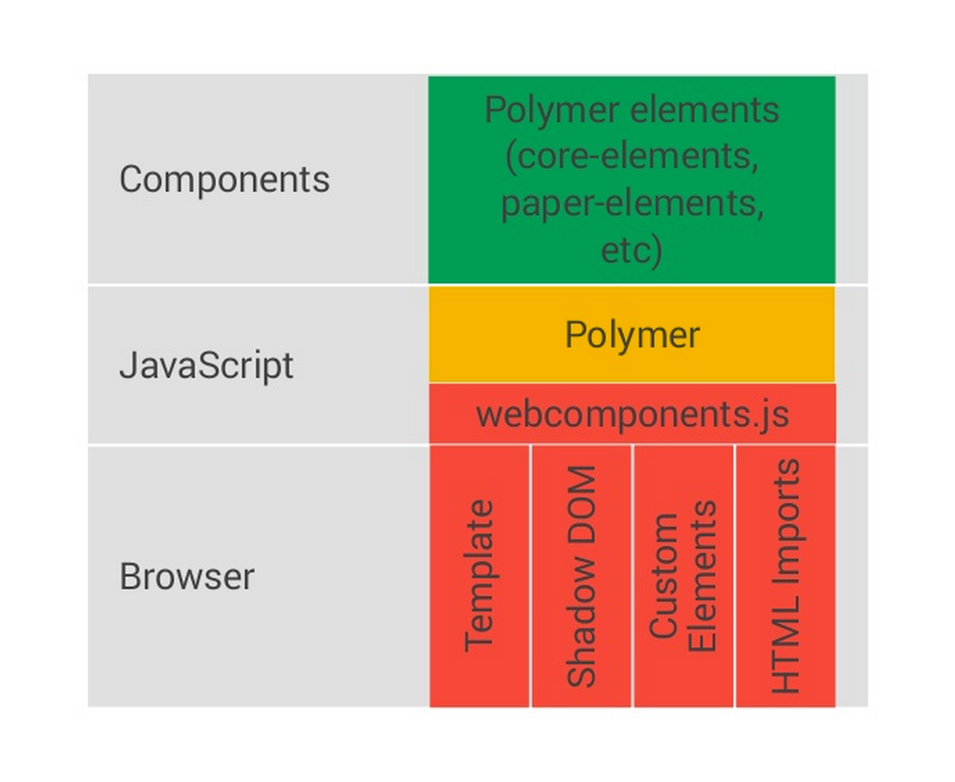
\includegraphics[width=7cm,keepaspectratio]{kapitel3/bilder/1-architektur}
 \caption{Schichtenmodell von Polymer}
 \label{fig:schimopo}
\end{figure}


\section{Elemente-Katalog}\label{elemente-katalog}

Der von Google verwaltete Elemente-Katalog verkörpert die Polymer-Philosophie ``There is an element for that'' \cite{citeulike:13930590}. Sie bilden eine Sammlung an Komponenten, welche die von Google vorgeschlagenen Implementierungen als Lösungen von einfachen bis komplexen wiederkehrenden Problemen sind. Entwickler können diese in ihrer eigenen Applikation optional einsetzen, sie sind beim Einsatz von Polymer aber nicht zwingend notwendig. Es werden dabei allerlei Anwendungsmöglichkeiten behandelt, von \ac{DOM}-Rendering in Form von Animationen, über Browser-\ac{API}-Interaktionen durch Push-Nachrichten, bis hin zu Remote-\ac{API}-Interaktionen mittels einem \ac{XHR}. Der Katalog besteht aus 7 Kategorien (Stand Januar 2016), welche die Komponenten nach Anwendungsfällen sortieren. Nachfolgend werden die Kategorien aufgelistet und erläutert.



\begin{description}
  \item[Iron Elements - Fe] Eisen ist der Kern der Erde. Daran orientiert sich die Metapher der Iron Elements, welche den Kern von Polymer und das Zentrum der Polymer Elemente bilden. Sie sind die wichtigsten Elemente, welche in vielen Projekten benötigt werden.
  \item[Paper Elements - Md] Die Paper Elements sind Googles-Design-Philosophie ``Material Design'' gehorchende Elemente wie Listen, Menüs, Tabs. Sie ermöglichen das Erstellen einer \ac{UI}. Paper ist dabei eine Metapher für ein erweitertes Papier, es kann zusammengesteckt werden, sich transformieren oder Schatten werfen.
  \item[Google Web Components - Go] Um die eigenen Services leichter verwendbar zu machen, stellt Google die Google Web Components bereit. Sie kapseln diese Services und \ac{API}s in Komponenten, wodurch Google Maps oder auch Google Drive usw. in der eigenen Applikation eingebunden und verwendet werden können.
  \item[Gold Elements - Au] Die Gold Elements sind eine Sammlung an buchstäblich wertvollen, goldenen Elementen, welche im Bereich E-Commerce eingesetzt werden können. Sie sind Komponenten für das Arbeiten mit Zahlungsmethoden oder Kreditkarteninformationen und können dabei Helfen, die Conversion-Rate der Applikation zu erhöhen.
  \item[Neon Elements - Ne] Die Neon Elements sind neben den Paper Elements auf \ac{UI}-Ebene einsetzbar. Mit ihnen können beispielsweise Animationen erstellt werden.
  \item[Platinum Elements - Pt] Wie die Gold Elements sind auch die Platinum Elements sehr wertvoll, jedoch in einer anderen Hinsicht. Sie sind nicht kommerziell orientiert, sondern für im Hintergrund laufende Services wie Push- oder Offline-Funk\-tio\-na\-li\-tä\-ten etc. gedacht. Sie sind Lösungen für sehr schwer lösbare, komplexe Probleme.
  \item[Molecules - Mo] Die Molecules sind weitere Elemente in Form von Wrappern für third-party-Lib\-rar\-ies.
  \item[Carbon Elements - C (in Entwicklung)] Die Carbon Elements befinden sich zum Stand dieser Arbeit noch in Entwicklung und sind noch nicht fertiggestellt. Sie sind metaphorisch sehr gewichtige Elemente und besitzen die Fähigkeit zur Bildung komplexer Moleküle, die essenziell für lebende Strukturen sind. Im übertragenen Sinn sind sie framework-orientierte Elemente und werden sich um strukturelle Probleme auf Applikations-Ebene kümmern.
\end{description}


\section{Alternative Sammlung von Komponenten}\label{alternative-sammlung-von-komponenten}

Statt den Polymer-Komponenten können auch selbst entwickelte oder aus anderen Quellen stammende Komponenten in eigenen Projekten verwendet werden. Der Elemente-Katalog wird dabei nur von Google vertrieben und erlaubt keine nicht von Google entwickelten Komponenten. Als eine Alternative für den Polymer Elemente-Katalog kann der customelements.io-Katalog \cite{citeulike:13926020} herangezogen werden. In diesem sind bereits mehrere tausend Komponenten gesammelt, welche von Google-unabhängigen Entwicklern für die unterschiedlichsten Anwendungsfälle entwickelt wurden.


\chapter{Analogie zu nativen Web Components}\label{analogie-zu-nativen-web-components}

In erster Linie vereinfacht Polymer das Erstellen und den Umgang mit Custom Elements, wobei versucht wird die von den Web-Components-Standards definierten Prämissen einzuhalten und zu erweitern. Ebenso wie bei dem nativen Erzeugen einer eigenen Komponente, werden bei Polymer für jede Komponente einzelne \ac{HTML}-Dateien erstellt, welche die Elemente repräsentieren. Darin werden alle JavaScript-, \ac{CSS}- und \ac{HTML}-Strukturen gesammelt und gekapselt. Man distanziert sich somit von der Code-Trennung, stattdessen werden alle Element-spezifischen Inhalte in einer Datei gebündelt. Wie das funktioniert und wie die Technologien mit Polymer umgesetzt werden, wird in diesem Kapitel dargestellt. In Abschnitt \ref{polymer-custom-elements} werden dabei die Custom Elements erläutert, in Abschnitt \ref{shadow-dom-und-html-templates} der Shadow \ac{DOM} zusammen mit den \ac{HTML} Templates und in Abschnitt \ref{polymer-html-imports} schließlich die \ac{HTML} Imports.


\section{Custom Elements}\label{polymer-custom-elements}

Die Intention der Polymer-Library ist das Erstellen eigener Komponenten oder Elemente, den Custom Elements. Das Erstellen, Erweitern und Verwalten von Custom Elements kann mit den nativen Mitteln bei steigender Komplexität mitunter schwierig werden. Polymer stellt hierfür eine Reihe an hilfreicher Funktionen bereit, welche das Arbeiten mit den Web-Components-Standards erleichtern und erweitern sollen \cite{citeulike:13915080}.


\subsection{Neues Element registrieren}\label{neues-element-registrieren}

Mit der Funktion \texttt{Polymer(pro\-to\-type);} können mit Polymer neue Elemente registriert werden, in dieser werden die generellen Polymer-Einstellungen in Form eines Prototyp-Objektes vorgenommen. Um ein Element zu definieren, muss der zu übergebende Prototyp die Eigenschaft \texttt{is:'element-name'} haben, welche den \ac{HTML}-Tag-Name des zu erstellenden Custom Elements angibt (in diesem Fall \texttt{element-name}). Der Name muss dabei als String übergeben werden und ebenso wie beim nativen Erzeugen eines Custom Elements einen Bindestrich enthalten. Die Polymer-Funktion registriert beim Aufruf automatisch das neue Element und gibt einen Konstruktor zurück, mit dem das Element instanziiert werden kann. Dies geschieht imperativ und deklarativ analog zu dem Erstellen mit der nativen Anweisung \texttt{var\ element\ =\ document.createElement('element-name');} bzw. mit dem zurückgegebenen Konstruktor oder im \ac{HTML}-Markup mit dem erstellten \ac{HTML}-Tag \texttt{\textless{}element-name\textgreater{}\textless{}/element-name\textgreater{}}. Soll statt dem Standard-Konstruktor ein Konstruktor erstellt werden, dem Argumente übergeben werden können, so muss in dem Prototyp die Methode \texttt{factoryImpl} mit den entsprechenden Argumenten definiert werden. Diese löst nach dem Ausführen einen \texttt{factoryImpl}-Callback (siehe Abschnitt \ref{neues-element-registrieren}) aus. Die \texttt{factoryImpl}-Methode wird allerdings nur aufgerufen, wenn ein Element mit dem zurückgegebenen Konstruktor, nicht jedoch beim Verwenden der \texttt{document.createElement}-Methode oder durch \ac{HTML}-Markup erzeugt wird.


\subsection{Elemente erweitern}\label{elemente-erweitern}

Ebenso wie nativ erzeugte Custom Elements können auch mit Polymer erzeugte Elemente die nativen Elemente erweitern, was unter Polymer ebenso als ``Type Extension Custom Element'' bezeichnet wird. Jedoch kann ein Polymer-Element nur native Elemente erweitern, andere Polymer-Elemente hingegen noch nicht. Dies soll allerdings in einer zukünftigen Version möglich sein. Das Erweitern und Erzeugen eines ``Type Extension Custom Elements'' funktioniert mit Polymer analog zu der nativen Methode. Hierzu muss im Prototyp die Eigenschaft \texttt{extends:\ '\ac{HTML}Element'} gesetzt werden, wobei das \texttt{'\ac{HTML}Element'} ein natives \ac{HTML}-Element wie z.B. \texttt{input} oder \texttt{button} sein muss. Zum Erzeugen des Elements kann nun wieder entweder die imperative Methode (siehe Abschnitt \ref{neues-element-registrieren}) oder die deklarative Methode analog dem nativen Erstellen mit \texttt{\textless{}\ac{HTML}Element\ is=\dq my-\ac{HTML}Element\dq\textgreater{}} mittels dem \texttt{is} Attribut, gewählt werden.


\subsection{Declared Properties -- Eigenschaften und Methoden definieren}\label{declared-properties---eigenschaften-und-methoden-definieren}

Custom Elements können auch mit Hilfe von Polymer um Eigenschaften und Methoden erweitert werden. Hierzu bietet Polymer das \texttt{properties}-Objekt an, mit welchem die Eigenschaften der Komponente im JSON-Format definiert werden können. Im Gegensatz zu den nativen Methoden, muss somit nicht jede Eigenschaft bzw. Property einzeln hinzugefügt werden. Die in diesem Objekt definierten Properties können beim Verwenden der Komponente im \ac{HTML}-Markup konfiguriert werden. Dadurch ist es möglich, eine \ac{API} für das Element zu erstellen, da die von außen konfigurierbaren Attribute ein Interface der Komponente bilden. Eine Property kann dabei mit folgenden Parametern spezifiziert werden.

\begin{description}
  \item[type] Konstruktor-Typ der Property, er kann ein Boolean, Date, Number, String, Array oder Object sein.
  \item[value] Standardwert der Property, der Wert muss boolean, number, string oder eine Funktion sein.
  \item[reflectToAttribute] Boolean-Wert, gibt an ob die Property mit dem \ac{HTML}-Attribut synchronisiert werden soll. Das bedeutet, falls die Property geändert wird, das zugehörige \ac{HTML}-Attribut des Elements geändert wird, was dem Funktionsaufruf \texttt{this.setAttribute(property,\ value);} entspricht. Dabei muss der Name des \ac{HTML}-Attributs in dem Properties-Objekt kleingeschrieben werden. Enthält der Name zusätzlich Bindestriche, so muss die Property kleingeschrieben und die Bindestriche entfernt werden, wobei jedes Wort nach einem Bindestrich groß geschrieben werden muss.
  \item[readOnly] Boolean-Wert, gibt an ob die Property nur gelesen oder auch geschrieben werden soll (siehe Abschnitt \ref{one-way--und-two-way-data-binding}).
  \item[notify] Boolean-Wert, die Property ist für Two-Way-Data-Binding (siehe Abschnitt \ref{one-way--und-two-way-data-binding}) verfügbar, falls true gesetzt ist. Zusätzlich wird ein \texttt{property-name-changed}-Event ausgelöst, wenn sich die Property ändert.
  \item[computed] Name der Funktion als String, welche den Wert der Property berechnen soll (siehe Abschnitt \ref{computed-properties}).
  \item[observer] Name der Funktion als String, welche aufgerufen wird, wenn der Wert der Property geändert wird (siehe Abschnitt \ref{property-oberserver}).
\end{description}

Die genannten Parameter sind alle optional anzugeben. Wird keine der Parameter definiert, so kann die Property direkt mit dem \texttt{type} definiert werden. Soll also beispielsweise eine Property \texttt{propertyName} als String und ohne Parameter angegeben werden, so würde dies mit \texttt{properties:\ \{\ propertyName:\ String\ \}} erreicht werden.


\subsection{Computed Properties}\label{computed-properties}

Polymer unterstützt des Weiteren zusammengesetzte, virtuelle Properties, welche aus anderen Properties berechnet werden. Um dies zu erreichen, muss die dafür verwendete Funktion im \texttt{properties}-Objekt mit entsprechenden Parametern angegeben werden. Soll beispielsweise die virtuelle Property \texttt{result} die Zusammensetzung der Properties a und b darstellen, so wird sie als \texttt{result:\ \{\ type:\ String,\ computed:\ computeResult(a,\ b)\ \}} im \texttt{properties}-Objekt angegeben. Die entsprechende Funktion muss dann als \texttt{computeResult:\ function(a,\ b)\ \{\ ...\ \}} im Polymer-Prototyp definiert werden. Diese wird einmalig aufgerufen, wenn sich eine der Eigenschaften a oder b ändert und wenn keine von beiden undefiniert ist. Der von ihr zurückgegebene Wert wird anschließend in der Variable \texttt{result} gespeichert.


\subsection{Property Oberserver}\label{property-oberserver}

Wird für eine Property der Parameter \texttt{observer} angegeben, so wird sie auf Änderungen überwacht. Die angegebene Funktion, welcher als optionale Argumente der neue und alte Wert übergeben werden können, wird somit aufgerufen, falls der Wert der Property geändert wird. Allerdings kann in dem \texttt{properties}-Objekt jeweils nur eine Property von einem Observer überwacht werden. Sollen mehrere Properties von demselben Observer überwacht werden, kann das \texttt{observers}-Array des Polymer-Prototyps verwendet werden. Soll beispielsweise die Funktion \texttt{computeResult(a,\ b)} ausgeführt werden, sobald sich eine der Properties \texttt{a} oder \texttt{b} ändert, so kann diese Funktion in das Array übernommen werden. Jedoch wird die Funktion auch hier nur dann ausgeführt, wenn keiner der Werte undefiniert ist. Des Weiteren wird bei angegebenen Funktionen -- im Gegensatz zu den im \texttt{properties}-Objekt angegebenen Observern -- nur der neue Wert statt des neuen und des alten Werts übergeben. Mit dem \texttt{observers}-Array ist es auch möglich, Sub-Properties oder Arrays zu überwachen.

\subsection{Das hostAttributes-Objekt}\label{das-hostattributes-objekt}

Zusätzlich zu den Declared Properties können auch \ac{HTML}-Attribute im Polymer-Pro\-to\-typ definiert werden. Hierzu bietet Polymer das \texttt{hostAttributes}-Objekt an. Die darin angegebenen Schlüssel-Wert-Paare werden beim initialen Erstellen des Elements auf dessen Attribute abgebildet. Das \texttt{hostAttributes}-Objekt kann dabei alle \ac{HTML}-Attribute bis auf das \texttt{class}-Attribut definieren, darunter fallen beispielsweise die Attribute \mbox{\texttt{data-*}}, \texttt{aria-*} oder \texttt{href}. Wird im \texttt{hostAttributes}-Objekt beispielsweise das Attribut \texttt{selected} mit \texttt{true} definiert, wird es bei einem \texttt{my-element}-Element in Form von \texttt{\textless{}my-element\ selected\textgreater{}Item\textless{}/my-element\textgreater{}} ausgegeben. Wichtig ist hier die Serialisierung der Schlüssel-Wert-Paare. Wird ein String, Date oder Number als Wert übergeben, so werden diese als String serialisiert. Werden jedoch Arrays oder Objekte übergeben, so werden diese mittels \texttt{JSON.stringify} serialisiert. Boolean-Werte werden bei \texttt{false} entfernt und bei \texttt{true} angezeigt. Um Daten in der anderen Richtung von einem \ac{HTML}-Element an das \texttt{hostAttributes}-Objekt zu propagieren, muss auf eine alternative Syntax zugegriffen werden (siehe Abschnitt \ref{binden-von-nativen-attributen}).


\subsection{Lifecycle-Callback-Funktionen}\label{lifecycle-callback-funktionen}

Die nativen Lifecycle-Callback-Funktionen (siehe Abschnitt \ref{custom-element-lifecycle-callbacks}) werden ebenso von Polymer unterstützt. Diese können in dem Prototyp als Attribut bei ihrem normalen Namen oder in verkürzter Form angegeben werden, so heißt die \texttt{createdCallback}-Methode \texttt{created}, die \texttt{attachedCallback}-Methode heißt \texttt{attached} und so weiter. Soll beispielsweise die \texttt{created}-Methode definiert werden, so kann diese mit \texttt{created:\ function\ \{\ ...\ \}} in dem Prototyp angegeben werden. Zusätzlich bietet Polymer einen \texttt{readyCallback}, welcher aufgerufen wird, nachdem Polymer das Element erstellt und den lokalen \ac{DOM} initialisiert hat, also nachdem alle im lokalen \ac{DOM} befindlichen Elemente konfiguriert wurden und jeweils ihre \texttt{ready}-Methode aufgerufen haben. Sie ist besonders hilfreich, wenn nach dem Laden der Komponente dessen \ac{DOM} nachträglich manipuliert werden soll. Falls mit den Lifecycle-Callbacks gearbeitet wird, muss auf die richtige Anwendung der Reihenfolge geachtet werden. So werden die Callbacks eines Elements in der Reihenfolge \texttt{created}, \texttt{ready}, \texttt{factoryImpl} und \texttt{attached} ausgeführt.


\section{Shadow DOM und HTML Templates}\label{shadow-dom-und-html-templates}

Die bisher gezeigten Methoden ermöglichen das Erstellen einer Polymer-Komponente, die jedoch noch kein internes Markup beinhaltet. Wie bei den nativen Technologien können auch mit Polymer erzeugte Custom Elements um \ac{HTML}-Markup, das lokale \ac{DOM}, erweitert werden \cite{citeulike:13915080}. Hierzu dient das Polymer \texttt{\textless{}dom-module\textgreater{}}-Element, welches als ID den Wert der \texttt{is}-Property des Polymer-Prototyps haben muss. Das zu verwendende \ac{HTML}-Markup muss dann in einem \texttt{\textless{}template\textgreater{}}-Tag dem \texttt{\textless{}dom-module\textgreater{}} hinzugefügt werden. Auf das Klonen des Inhalts des Templates mittels der \texttt{importNode}-Funktion (siehe Abschnitt \ref{benutzung}) kann hierbei verzichtet werden, da Polymer diesen automatisch in den lokalen \ac{DOM} des Elements klont. Soll also das lokale \ac{DOM} des \texttt{\textless{}element-name\textgreater{}}-Tags deklariert werden, so wird dies wie in Listing \ref{tepk} dargestellt erreicht:

\lstinputlisting[language=HTML,label=tepk,caption=Template einer Polymer-Komponente]{kapitel4/listings/1-1.html}

Der deklarative Teil des Elements, das \texttt{\textless{}dom-module\textgreater{}} und dessen Inhalte, sowie der Imperative Teil mit dem \texttt{Polymer(\{\ ...\ \})}-Aufruf können entweder in derselben oder in getrennten \ac{HTML}-Dateien stehen. Hierbei spielt es jedoch keine Rolle, ob das \texttt{\textless{}script\textgreater}-Tag innerhalb oder außerhalb des \texttt{\textless{}dom-module\textgreater{}}-Tags steht, solange das Template vor dem Polymer-Funktionsaufruf geparst wird.


\subsection{Shady DOM}\label{shady-dom}

Wie in Abschnitt \ref{shadow-dom-browserunterstuetzung} gezeigt, wird das Shadow \ac{DOM} nicht von allen Browsern unterstützt. Ebenso ist der Polyfill für dieses, aufgrund dessen schlechter Performance (siehe Abschnitt \ref{performance}), nur als allerletzte Instanz zu sehen. Aus diesen Gründen ist in Polymer das sogenannte ``Shady \ac{DOM}'' implementiert \cite{citeulike:13886251}. Dieses bietet einen dem Shadow \ac{DOM} ähnlichen Scope für den \ac{DOM}-Tree. Dabei rendert er das \ac{DOM}, als wenn kein Shadow \ac{DOM} in dem Element vorhanden wäre. Dies bringt wiederum auch die dadurch entstehenden Nachteile mit sich, wie dass internes Markup nach außen sichtbar ist oder keine Shadow Boundary verfügbar ist. Der Vorteil ist jedoch, dass das Shady \ac{DOM} genug Methoden für seinen Scope bereitstellt, um sich wie ein Shadow \ac{DOM} verhalten zu können, ohne die Performance zu mindern. Hierzu ist es jedoch zwingend notwendig, die eigens entwickelte Shady-\ac{DOM}-\ac{API} im Umgang mit dem \ac{DOM} zu benutzen, was mit der \texttt{Polymer.dom(node)}-Funktion erreicht wird. Will man beispielsweise alle Kinder mit der \texttt{children}-Eigenschaft des Shadow-Host-Elements \texttt{\textless{}my-element\textgreater{}} selektieren, so erfolgt dies mit das Shady-\ac{DOM}-\ac{API} mittels \texttt{var\ children\ =\ Polymer.dom(my-element).children;} statt mit der normalen \ac{DOM}-\ac{API} mittels \texttt{var\ children\ =\ document.getElementsByTagName(\dq my-element\dq){[}0{]}.children;}. Diese gibt dann nur die von außen übergebenen (Light-\ac{DOM}-)Elemente zurück, ohne die Elemente des internen Markups des Templates zu berücksichtigen. Die Shady-\ac{DOM}-\ac{API} bildet dabei alle Funktionen der nativen \ac{DOM}-\ac{API} ab und ist performanter als der Shadow-\ac{DOM}-Polyfill, da nicht dessen Verhalten, sondern nur ein eigener \ac{DOM}-Scope implementiert ist. Jedoch beschränkt sich Polymer nicht nur auf den eigenen Shady \ac{DOM}, vielmehr ist es mit dem nativen Shadow \ac{DOM} kompatibel, sodass die Shady-\ac{DOM}-\ac{API} auf das native Shadow \ac{DOM} zugreifen kann, falls dieses von dem Browser unterstützt wird. Dadurch kann eine Applikation implementiert werden, die auf allen Plattformen mit einer verbesserten Performance ausgeführt wird, wovon besonders die mobilen Plattformen profitieren. Standardmäßig benutzt Polymer jedoch immer die eigene Shady-\ac{DOM}-\ac{API}, wie das verhindert werden kann, ist in Abschnitt \ref{optimierungen-fuxfcr-eine-fluxfcssige-applikation} dargestellt.


\subsection{DOM-Knoten automatisch finden}\label{dom-knoten-automatisch-finden}

Um das Traversieren in dem lokalen \ac{DOM} zu beschleunigen, bietet Polymer eine Hilfsfunktion für das automatische Finden eines Elements, auch ``Automatic Node Finding'' genannt, an. Hierzu wird intern ein Mapping zu den statisch erzeugten \ac{DOM}-Elementen erzeugt, indem jedes Element des lokalen \ac{DOM}-Templates, für welches eine ID definiert wurde, in dem \texttt{this.\$}-Hash gespeichert wird. Hat nun also beispielsweise das Element \texttt{\textless{}div\ id=\dq wrapper\dq\textgreater{}\textless{}/div\textgreater{}} in dem Template die ID \texttt{wrapper}, so kann es in Polymer mittels \texttt{this.\$.wrapper} selektiert werden. Jedoch werden dem Hash nur die statisch erzeugten \ac{DOM}-Knoten hinzugefügt, dynamisch mittels \texttt{dom-repeat} oder \texttt{dom-if} hinzugefügte Knoten allerdings nicht. Die dynamisch hinzugefügten Knoten können mit der \texttt{this.\$\$}-Funktion selektiert werden. So liefert die Funktion \texttt{this.\$\$(selector);} das erste Element, welches von den im Parameter \texttt{selector} enthaltenen \ac{CSS}-Selektor selektiert wird.


\subsection{Content Projection}\label{polymer-content-projection}

Um nun Elemente des Light \ac{DOM}s in das lokale \ac{DOM} der Komponente zu injizieren, bietet Polymer ebenso das von den nativen Methoden bekannte \texttt{\textless{}content\textgreater{}}-Element an, welches einen Insertion Point des Light \ac{DOM}s im lokalen \ac{DOM} der Komponente darstellt. Wie auch bei den nativen Insertion Points kann das \texttt{\textless{}content\textgreater{}}-Element auch nur selektierte Inhalte injizieren, indem das \texttt{select}-Attribut mit einem entsprechenden Selektor gesetzt wird. Falls das Shadow \ac{DOM} in Polymer verfügbar ist, so wird eine Zusammenstellung des Shadow \ac{DOM}s und dem Light \ac{DOM} gerendert. Ist das Shadow \ac{DOM} jedoch nicht verfügbar und das Shady \ac{DOM} wird verwendet, so ist das zusammengesetzte \ac{DOM} das tatsächliche \ac{DOM} des Elements. Auch kann in Polymer mittels der \texttt{\_observer}-Eigenschaft überwacht werden, ob Kind-Elemente der Komponente hinzugefügt oder von ihr entfernt werden. Dazu wird dieser die Funktion \texttt{observeNodes(callback)} zugewiesen, welche ausgeführt wird, wenn Elemente hinzugefügt oder entfernt werden. Der Parameter \texttt{callback} ist dabei eine anonyme Funktion, welche als Übergabewert das Objekt \texttt{info} hat, in welchem die hinzugefügten oder entfernten Knoten enthalten sind. Eine Implementierung der Überwachung des \texttt{contentNode}-Knotens auf Änderungen könnte dabei wie in Listing \ref{uebecnk} dargestellt aussehen.

\lstinputlisting[language=JavaScript,label=uebecnk,caption=Überwachung eines \texttt{contentNode}-Knotens]{kapitel4/listings/1-2.js}


\subsection{CSS-Styling}\label{css-styling}

Die in Abschnitt \ref{styling-mit-css} gezeigten Regeln für das Stylen des Shadow \ac{DOM}s sind auch unter Polymer und dessen Shady \ac{DOM} gültig \cite{citeulike:13915080}. Zusätzlich können Komponenten \ac{CSS}-Properties (also Variablen) nach außen sichtbar machen, damit diese von außerhalb der Komponente gesetzt werden können. Somit kann das \ac{CSS} in einer gekapselten Komponente bestimmt werden. Hierbei können auch Standardangaben gemacht werden, die von der Komponente übernommen werden, wenn die Variable nicht definiert wird. Um eine Variable bereitzustellen, muss diese der entsprechenden Eigenschaft mit der Syntax \texttt{var(-\/-variable-name,\ default)} in den Style-Regeln der Komponente angegeben werden. Das Beispiel in Listing \ref{xelementkmcssv} zeigt das \ac{DOM} eines \texttt{x-element}, welches die \ac{CSS}-Variable \texttt{x-element-button-color} und dem zugewiesenen Standardwert \texttt{red} für einen Button in einem \texttt{\textless{}div\textgreater{}}-Tag mit der Klasse \texttt{x-element-container} bereitstellt.

\lstinputlisting[language=HTML,label=xelementkmcssv,caption=\texttt{x-element}-Komponente mit einer \ac{CSS}-Variablen]{kapitel4/listings/1-3.html}

Die Applikation, welche die Komponente benutzt, kann nun die Variable \texttt{-\/-x-element-button-color} definieren, wie in Listing \ref{ddcssv} gezeigt wird.

\lstinputlisting[language=HTML,label=ddcssv,caption=Definition der \ac{CSS}-Variable]{kapitel4/listings/1-4.html}

Das Attribut \texttt{is=\dq custom-style\dq} des \texttt{\textless{}style\textgreater{}}-Tags dient dabei als Anweisung für den Polyfill, da \ac{CSS}-Properties noch nicht von allen Browsern unterstützt werden. Nun soll jedoch nicht für jedes \ac{CSS}-Attribut eine Variable angelegt werden, da dies schnell unübersichtlich werden kann. Um mehrere \ac{CSS}-Attribute einer Komponente ändern zu können, können sogenannte Mixins erstellt werden. Diese sind eine Sammlung an Styles, die auf eine Komponente angewendet werden können. Sie werden wie eine \ac{CSS}-Variable definiert, mit dem Unterschied, dass der Wert ein Objekt ist, welches ein oder mehrere Regeln definiert. Um ein Mixin nach außen bereitzustellen, muss es in der Komponente in den \ac{CSS}-Regeln mit \texttt{@apply(-\/-mixin-name)} bereitgestellt werden. Es kann dann von der Applikation verwendet werden. So kann das obige Beispiel um das \texttt{-\/-x-element}-Mixin erweitert werden (siehe Listing \ref{edsuem}).

\lstinputlisting[language=HTML,label=edsuem,caption=Erweiterung der Styles um ein Mixin]{kapitel4/listings/1-5.html}

Wobei es wie in Listing \ref{vemek} dargestellt von der einsetzenden Applikation konfiguriert werden könnte.

\lstinputlisting[language=HTML,label=vemek,caption=Verwendung eines Mixins einer Komponente]{kapitel4/listings/1-6.html}


\subsection{Gemeinsame Styles mehrerer Komponenten}\label{gemeinsame-styles-mehrerer-komponenten}

Um nun Style-Regeln auf mehrere Komponenten anzuwenden, stellt Polymer die sogenannten ``Style Modules'' bereit. Diese ersetzen die ab Version 1.1 nicht mehr \mbox{unterstützte} Möglichkeit, externe Stylesheets zu verwenden. Style Modules sind dabei nichts anderes als Komponenten, welche von allen Komponenten importiert werden können, die diese Styles anwenden sollen.


\subsubsection{Style Module anlegen}

Um eine Komponente mit geteilten Style-Regeln zu erstellen, genügt es, dass diese die Style-Regeln in einem \texttt{\textless{}dom-module\textgreater{}}-Tag mit einer beliebigen ID definiert. Dies wird in dem Listing \ref{htmldsshtml} der Datei ``shared-styles.html'' gezeigt. Darin wird eine Style-Regeln definiert, die den Text aller Elemente mit der Klasse \texttt{wrapper} rot anzeigen lässt.

\lstinputlisting[language=HTML,label=htmldsshtml,caption=\ac{HTML}-Datei ``shared-styles.html'']{kapitel4/listings/1-7.html}


\subsubsection{Style Module benutzen}

Damit eine Komponente diese Styles nutzen kann, muss sie sie zunächst importieren und anschließend einen \texttt{\textless{}style\textgreater{}}-Tag definieren, welcher als \texttt{include}-Attribut den Namen der Komponente mit den geteilten Style-Regeln hat. Die Styles werden darin importiert und auf die gesamte Komponente angewendet. Somit wird der Text des \texttt{\textless{}div\textgreater{}}-Tags mit der Klasse \texttt{wrapper} rot dargestellt (siehe Listing \ref{besm}).

\lstinputlisting[language=HTML,label=besm,caption=Benutzung eines Style-Moduls]{kapitel4/listings/1-8.html}


\newpage
\section{HTML Imports}\label{polymer-html-imports}

Um mehrere Polymer Komponenten oder Komponenten innerhalb anderer Komponenten zu benutzen, verwendet Polymer \ac{HTML} Imports. Diese funktionieren analog zu der Verwendung mit der nativen \ac{HTML} Imports Technologie (siehe Abschnitt \ref{html-imports}), wobei die selben Vor- und Nachteile auftreten. Polymer kümmert sich dabei lediglich automatisch im Hintergrund um die korrekte Einbindung der \ac{HTML}-Dateien und dessen Bereitstellung im Dokument, falls ein \texttt{\textless{}link\ rel=\dq import\dq\textgreater{}} in einer Komponente enthalten ist. Das manuelle Einbinden mittels der speziellen JavaScript-Methoden oder Eigenschaften, wie beispielsweise der \texttt{import}-Eigenschaft des importierten Elements, wird somit hinfällig.

\subsection{Dynamisches Nachladen von HTML}\label{dynamisches-nachladen-von-html}

Falls \ac{HTML}-Dateien dynamisch zur Laufzeit nachgeladen werden sollen, bietet Polymer zusätzlich eine Hilfsfunktion an, mit der \ac{HTML} Imports nachträglich ausgeführt werden können \cite{citeulike:13914840}. Die hierfür bereitgestellte Hilfsfunktion \texttt{importHref(url,\ onload,\ onerror);} importiert beim Aufruf dynamisch die angegebene \ac{HTML}-Datei in das Dokument. Sie erstellt dabei ein \texttt{\textless{}link\ rel=\dq import\dq\textgreater{}}-Element mit der angegeben URL und fügt es dem Dokument hinzu, sodass dieser ausgeführt werden kann. Wenn der Link geladen wurde, also der \texttt{onload}-Callback aufgerufen wird, ist die \texttt{import}-Eigenschaft des Links der Inhalt des zurückgegebenen, importierten \ac{HTML}-Dokuments. Der Parameter \texttt{onerror} ist dabei eine optionale Callback-Funktion, die beim Auftreten eines Fehlers aufgerufen wird.


\chapter{Zusätzliche Polymer Funktionalitäten}\label{zusaetzliche-polymer-funktionalitaeten}

Polymer bietet eine zusätzliche Applikations-Schicht mit einigen hilfreichen Funktionalitäten, die das Arbeiten mit den Komponenten vereinfachen. Die wichtigsten werden in diesem Kapitel dargestellt. Abschnitt \ref{one-way--und-two-way-data-binding} widmet sich dabei um das One-Way- und Two-Way-Data-Binding, Abschnitt \ref{behaviors} erläutert die Behaviors und in Abschnitt \ref{events} erklärt abschließend die Events.


\section{One-Way- und Two-Way-Data-Binding}\label{one-way--und-two-way-data-binding}

Für den Transport von Daten zwischen Komponenten sieht Polymer das One-Way- und Two-Way-Data-Binding vor. Die Daten können dabei zwischen einer Eigenschaft eines Custom Elements (Host-Element) und dessen lokalen \ac{DOM} (Kind-Element) gebunden und somit zwischen Komponenten ausgetauscht werden. Hierfür sieht Polymer das Mediator-Pattern vor, welches besagt, dass Daten zwischen 2 nebenstehenden Komponenten ihre Daten über eine übergeordnete Komponente propagieren müssen. Dies erfolgt mittels einer hierfür vorgesehenen Syntax für Attribute eines Elements, wie zum Beispiel: \texttt{\textless{}my-element\ some-property=\{\{value\}\}\textgreater{}\textless{}/my-element\textgreater{}}. Durch die doppelten Klammern kann die Eigenschaft \texttt{value} des Host Elements Daten in das Attribut \texttt{some-property} des Kind Elements weitergeben. Hierzu wird von Polymer für jede Eigenschaft eines Elements ein \texttt{propertyEffect} Objekt und ein entsprechender Setter angelegt. Wenn die Eigenschaft zur Laufzeit geändert wird, wird über das Array aus propertyEffects iteriert und bei entsprechender Eigenschaft mittels dem Setter der neue Wert gesetzt, falls dieser sich von dem alten Wert unterscheidet. Wird die Eigenschaft von einem Observer (siehe Abschnitt \ref{property-oberserver}) überwacht, so wird dieser im Setter aufgerufen, statt die Werte direkt zu ändern. Für das Binden stehen unterschiedlichen Annotationen zur Verfügung, welche nachfolgend erläutert werden \cite{citeulike:13914892}.


\subsection{One-Way-Data-Binding}\label{one-way-data-binding}

Das One-Way-Data-Binding erlaubt Attributen nur das Lesen der entsprechenden Eigenschaft seiner Komponente, ein schreibender Zugriff wird jedoch untersagt. Meist wird es verwendet, um Texte basierend auf einer Eigenschaft anzuzeigen, der Text jedoch soll nicht verändert werden oder die Eigenschaft überschreiben. Erreicht wird das One-Way-Data-Binding mit der doppelten eckigen Klammer Syntax \texttt{{[}{[}{]}{]}}. Intern legt Polymer für die Eigenschaft keinen eventListener \texttt{attributeName-changed} für das Attribut \texttt{attributeName} an, somit wird die Eigenschaft, falls das Attribut geändert werden sollte, nicht upgedatet. Beim One-Way-Data-Binding kann dabei zwischen 2 Möglichkeiten unterschieden werden.


\textbf{Host to Child}

Das Transportieren der Daten erfolgt nur von Host-Element zum Kind-Element. Hierzu muss zusätzlich der \texttt{readOnly}-Parameter (siehe Abschnitt \ref{declared-properties---eigenschaften-und-methoden-definieren}) nicht definiert oder mit \texttt{false} initialisiert werden.

\textbf{Child to Host}

Der Transport der Daten erfolgt nur von Kind-Element zu Host-Element. Hierzu müssen die \texttt{notify}- und \texttt{readOnly}-Parameter mit \texttt{true} initialisiert werden.


\subsection{Two-Way-Data-Binding}\label{two-way-data-binding}

Mittels dem Two-Way-Data-Binding, auch ``automatic Binding'' genannt, können Daten von Host- zu Kind-Element und umgekehrt geschrieben werden. Hierzu ist es zwingend notwendig, den \texttt{notify}-Parameter mit \texttt{true} zu initialisieren und zusätzlich die doppelte geschweifte Klammer Syntax \texttt{\{\{\}\}} zu verwenden. Sobald eine der beiden Eigenschaften, die des Kindes oder die des Hosts, geändert werden, wird von dem jeweiligen Element ein \texttt{propertyName-changed-event} abgefeuert. Wenn nun ein anderes Element an diese Eigenschaft gebunden ist, bekommt es das Event mit und ändert daraufhin den eigenen Wert. Hierdurch ist es möglich, eine \ac{API} für eine Komponente bereit zu stellen, um Daten nach außen sichtbar zu machen. Somit können Daten zwischen 2 oder mehr Komponenten ausgetauscht werden.


\subsection{Binden von nativen Attributen}\label{binden-von-nativen-attributen}

Um Werte an von \ac{HTML} reservierte Attribute, also das \texttt{hostAttributes}-Objekt (siehe Anschnitt 3.2) statt an Eigenschaften der Komponente zu binden (was mit der normalen Attribut-Binding-Syntax \texttt{=} erreicht wird), muss die hierfür vorgesehene Syntax \texttt{=\$} verwendet werden. So wird beispielsweise in dem Element \texttt{\textless{}div\ class=\$\dq \{\{myClass\}\}\dq\textgreater{}\textless{}/div\textgreater{}} die Eigenschaft \texttt{myClass} tatsächlich dem Attribut \texttt{class} statt der Eigenschaft zugewiesen. Polymer wandelt hierbei bei Verwendung der \texttt{=\$} Syntax die Zuweisung in die Anweisung \texttt{\textless{}div\textgreater{}.setAttribute('class',\ myClass);} um. Das Binden von nativen Attributen ist somit automatisch immer nur in eine Richtung von Host- zu Kind-Element. Im Allgemeinen sollte die Syntax immer dann verwendet werden, wenn die Attribute \texttt{style}, \texttt{href}, \texttt{class}, \texttt{for} oder auch \texttt{data-*} gesetzt werden sollen.


\section{Behaviors}\label{behaviors}

Auch wenn in Polymer nur ein beschränktes Vererben mit Hilfe von Type Extensions möglich ist, gibt es dennoch die Möglichkeit Komponenten mit geteilten Code-Modulen zu erweitern \cite{citeulike:13915080}. Diese Module werden innerhalb von Polymer Behaviors genannt. Behaviors erlauben es, einen Code in mehrere Komponenten einzubinden, um diese mit einem gewissen Verhalten oder mit zusätzlichen Funktionalitäten auszurüsten. Mit Hilfe der Behaviors haben Entwickler eine gute Kontrolle darüber, welche externen Codes in die eigene Komponente fließen. Sie können im Elemente-Katalog gefunden und eingesehen werden. Dort sind sie unter anderem in den Iron-Elementen mit Input-Validierungen oder in den Neon-Elementen mit Animationsverhalten auffindbar.


\subsection{Syntax}\label{syntax}

Behaviors sind globale Objekte und sollten in einem eigenem Namespace, wie z.B. mit \texttt{window.MyBehaviors\ =\ window.MyBehaviors\ \textbar{}\textbar{}\ \{\};}, definiert werden, da die von Polymer intern benutzten Behaviors im
Polymer-Objekt verankert sind. Dadurch können Kollisionen mit zukünftigen Behaviors von Polymer verhindert werden. Behaviors haben eine starke Ähnlichkeit zu normalen Polymer-Elementen, sie besitzen ebenso Properties, Listener-Objekte und so weiter. Ein simples Behavior könnte beispielsweise wie in Listing \ref{deb} dargestellt definiert werden \cite{citeulike:13915079}.

\lstinputlisting[language=JavaScript,label=deb,caption=Definition eines Behaviors]{kapitel5/listings/1-1.js}

Dieses Behavior würde, falls es von einer Polymer Komponente benutzt würde, einen Alert auslösen, wenn die Komponente geklickt wird. Um das Behavior nun einer Komponente hinzuzufügen, muss es dem Behaviors-Array hinzugefügt werden \texttt{Polymer(\{\ is:\ 'super-element',\ behaviors:\ {[}HelloBehavior{]}\ \});}. In diesem Array können so viele Behaviors mit unterschiedlichen Verhaltensweisen hinzugefügt werden, wie benötigt werden.


\subsection{Behaviors erweitern}\label{behaviors-erweitern}

Wie auch Komponenten wiederum andere Komponenten erweitern können, können ebenso Behaviors erweitert werden. Somit können auch Behaviors untereinander geteilte Funktionalitäten einbinden. Um ein Behavior zu erweitern, müssen zunächst alle Behaviors importiert werden, welche das neue Behavior beinhalten soll. Anschließend wird das Verhalten des neuen Behaviors implementiert. Um das neue Behavior nun tatsächlich mit den anderen Behaviors zu erweitern, wird es als Array aus den importieren Behaviors und dem neu implementieren Behavior definiert, wie in Listing \ref{eeb} dargestellt.

\lstinputlisting[language=HTML,label=eeb,caption=Erweiterung eines Behaviors]{kapitel5/listings/1-2.html}


\section{Events}\label{events}

Mit Polymer erstellte Komponenten können mit Hilfe des \texttt{listeners} Objekts auf bestimmte Interaktionen mit der Komponente reagieren {[}citeulike:13915080{]}. Hierzu wird die entsprechende Aktion mit der auszuführenden callBack Funktion in dem Objekt angegeben. Wird nun innerhalb der Komponente das angegebene Event registriert, wird die angegebene Funktion ausgeführt. Zu diesen Events zählen beispielsweise die Gesture Events, wie sie in Abschnitt \ref{gesture-system} beschrieben werden. Um nun verschiedene Aktionen mit unterschiedlichen Kind Elementen zu verknüpfen, können dem \texttt{listeners} Objekt auch Kind Elemente und dessen callBack Funktion mit der Syntax \texttt{nodeID.eventName:\ callBack()} hinzugefügt werden. Dadurch reagiert nur das angegebene Element auf das Event, statt der gesamten Komponente. So kann beim ``Tap'' auf ein Element mit der ID \texttt{nodeID} die Funktion (der Event Handler) \texttt{callBack()} aufgerufen werden.


\subsection{Deklarative Events}\label{deklarative-events}

Alternativ zur imperativen Definition von Events mittels dem \texttt{listeners} Objekt, können diese auch deklarativ im Markup des Elements im lokalen \ac{DOM} der Komponente angegeben werden. Will ein Element auf ein Event reagieren, so muss es dazu die \texttt{on-eventName} wie z.B. \texttt{\textless{}button\ on-tap=\dq handleTap\dq\textgreater{}Tap\ Button\textless{}/button\textgreater{}} Annotation benutzen, wodurch bei Tap auf den Button die Funktion \texttt{handleTap} ausgeführt wird. Dies vermischt zwar innerhalb des Templates \ac{HTML} und Javascript, jedoch muss mit dieser Methode dem Element keine ID zugewiesen werden, nur um dessen Event zu binden.


\subsection{Selbst definierte Events}\label{selbst-definierte-events}

Falls das gewünschte Event nicht existieren sollte, können von Host Elementen und dessen Kind Elementen auch selbst definierte Events ausgelöst werden. Hierfür muss von der Komponente die Hilfsfunktion \texttt{fire(eventName,\ data);} aufgerufen werden, welches wiederum von anderen Events ausgelöst werden kann. In Listing \ref{aesde} wird das Auslösen eines selbst erstellten Events mit der deklarativen Methode verdeutlicht. Der Button in Zeile 3 ruft die Funktion \texttt{postClick} auf, wenn er geklickt wird. Diese wiederum feuert mittels der Hilfsfunktion \texttt{fire} das Event \texttt{my-event}. Nun kann aus dem umschließenden Dokument, der eigenen Komponente oder aus anderen Komponenten auf das Event gehört werden, in dem die Funktion \texttt{addEventListener} (Zeile 17) auf das Event abfeuernde Element gebunden wird.

\lstinputlisting[language=HTML,label=aesde,caption=Auslösen eines selbst definierten Events]{kapitel5/listings/1-3.html}


\chapter{Best Practices beim Arbeiten mit Polymer}\label{best-practices-beim-arbeiten-mit-polymer}

In den vorherigen Kapiteln wurde gezeigt, welchen Mehrwert Polymer für die Entwickler bringt und wie die Library eingesetzt wird. In diesem Kapitel werden in Abschnitt \ref{ui-performance-patterns} einige \ac{UI}-Performance-Patterns für eine möglichst performante Applikation sowie in Abschnitt \ref{gesture-system} das Gesture-System erläutert. Abschnitt \ref{a11y---barrierefreiheit-in-polymer} erläutert die von Polymer bereitgestellten Mittel zum Entwickeln einer möglichst barrierefreien Applikation.


\section{UI-Performance-Patterns}\label{ui-performance-patterns}

Applikationen und Webseiten in dem modernen Web müssen möglichst schnell Laden sowie ein flüssiges Arbeiten ermöglichen, damit sie von den Benutzern akzeptiert und genutzt werden. In Abbildung \ref{fig:vwdbbul} wird deutlich, dass Applikationen mit einer Ladezeit von ca. 1000 Millisekunden oder mehr sich negativ auf die Zufriedenheit der Nutzer auswirken. \cite{citeulike:13262776}

\begin{figure}[htbp]
 \centering
 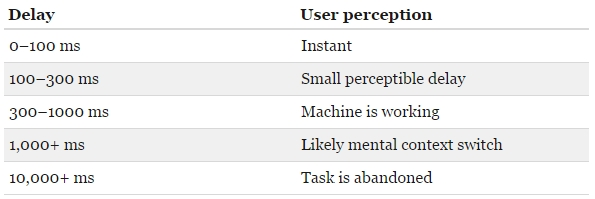
\includegraphics[width=11cm,keepaspectratio]{kapitel6/bilder/1-performance-user-perception-reaction-times}
 \caption{Wahrnehmungen der Benutzer bei unterschiedlichen Ladezeiten}
 \label{fig:vwdbbul}
\end{figure}


\subsection{Ladezeiten und initiales Rendern optimieren}\label{ladezeiten-und-initiales-rendern-optimieren}

Ohne ein besonderes Augenmerk auf die Performance zu werfen, bleibt die Seite oder die Applikation beim initialen Laden mitunter zunächst weiß und der Benutzer kann keine Inhalte sehen. Wenn alle Ressourcen fertig geladen sind, wird der Inhalt dann plötzlich und unerwartet eingeblendet. Dies wird durch blockierende Elemente verursacht. Das erste blockierende Element sind bereits die webcomponents.js Polyfills, da diese in einem \texttt{\textless{}script\textgreater{}}-Tag stehen und somit sequenziell geladen werden müssen und die Ladezeit verlängern. Dies kann jedoch verhindert werden, indem dem Tag das \texttt{async}-Attribut hinzugefügt wird, alle anderen Ressourcen können dann asynchron geladen werden und die Applikation muss nicht auf die Polyfills warten. Um die Ladezeit weiter zu verkürzen, kann mit JavaScript überprüft werden, ob die Polyfills optional geladen werden müssen (Lazy Load) (siehe Listing \ref{bfd}).

\lstinputlisting[language=JavaScript,label=bfd,caption=Browser-Feature-Detection]{kapitel6/listings/1-1.js}

Neben den Polyfills blockieren importierte \ac{HTML}-Dateien, also andere Komponenten, zwar nicht das Laden der Applikation, jedoch dessen Rendern, da diese selbst wiederum sowohl \texttt{\textless{}script\textgreater{}}-Tags als auch Stylesheets beinhalten. Des Weiteren blockieren diese das Rendern der Webseite, da der Browser die importieren \ac{CSS}-Dateien erst parsen muss. Hier kann ebenfalls das \texttt{async}-Attribut gesetzt werden um dieses Problem zu lösen. Somit wird die Webseite sofort nach dem Laden aller Ressourcen gerendert, jedoch auch ohne Anwendung der Style-Regeln. Der hierdurch entstehende \ac{FOUC} muss also manuell verhindert werden, indem grobe Container in einem \texttt{\textless{}style\textgreater{}}-Tag für das ungefähre Aussehen der Applikation definiert werden. Dadurch werden die Komponenten nach und nach in die Container geladen, es wird somit sofort eine Vorschau der Applikation angezeigt und die Applikation schnell geladen \cite{citeulike:13915203}.


\subsection{Optimierungen für eine flüssige Applikation}\label{optimierungen-fuxfcr-eine-fluxfcssige-applikation}

Wie in Abschnitt \ref{shady-dom} gezeigt, implementiert Polymer eine eigene Version des Shadow \ac{DOM}s, den Shady \ac{DOM}, um eine möglichst breite Browserunterstützung zu gewährleisten. Im Gegensatz zum Shadow \ac{DOM}, welcher im Kontext der Browser in der Programmiersprache C++ programmiert ist, ist der Shady \ac{DOM} nur eine in JavaScript programmierte Nachbildung dessen. Somit ist dieser schon auf Plattform-Ebene langsamer. Zusätzlich ist das Scoping sowie das Rendern im nativen Shadow \ac{DOM} einiges schneller. Vor dem Einbinden der Polymer-Library sollte somit im globalen \texttt{Polymer}-Settings-Objekt die Property \texttt{dom} auf den Wert \texttt{'shadow'} gesetzt werden. Polymer überprüft daraufhin, ob der Browser das Shadow \ac{DOM} unterstützt. Falls ja, wird dieses statt dem Shady DOM benutzt.

Um eine schnelle Reaktionszeit der Applikation zu gewährleisten, sollten statt Click-Events immer die Touch-Events verwendet werden (siehe Abschnitt \ref{gesture-system}), da Click-Events auf mobilen Geräten eine Zeitverzögerung von 300 Millisekunden haben, bevor diese tat\-s\"ach\-lich abgefeuert werden. Dies wird von den Browserherstellern so implementiert, da die Browser bei Click-Events zu erst prüfen müssen, ob das Event Teil eines Doppel-Taps ist, was einen Zoom auslösen würde.

Darüber hinaus sollten nicht benötigte Elemente nur dann tatsächlich gerendert werden, wenn diese auch wirklich im Viewport des Browsers zu sehen sind (Lazy Render). Wird dies nicht gemacht, werden alle Elemente beim initialen Laden der Seite gerendert, was die Applikation bei mehreren Tausend Elementen sehr träge machen kann. So setzt beispielsweise die \texttt{\textless{}iron-list\textgreater{}}-Komponente von Polymer diese Technik um, indem es nur die Elemente in das \ac{DOM} lädt, welche aktuell sichtbar sein müssen. Ebenso wird das lokale \ac{DOM} des \texttt{dom-if}-Templates \texttt{\textless{}template\ is='dom-if'\ if='\{\{open\}\}'\textgreater{}} nur dann generiert und gerendert, wenn das Element aktiv ist, also wenn \texttt{open} den Wert true annimmt. Dies kann unter anderem bei Dropdown Elementen oder Akkordeon-Menüs umgesetzt werden. Um zu prüfen, wie viele Polymer Komponenten aktuell auf der Seite im \ac{DOM} stehen und Informationen über dessen Performance zu erhalten, stellt Polymer die Erweiterung ``Polymer DevTools Extension'' für den Chrome-Browser zur Verfügung \cite{citeulike:13915202}.


\section{Gesture-System}\label{gesture-system}

Wie bereits in dem vorangegangenen Abschnitt \ref{ui-performance-patterns} angeschnitten wird, sind flüssige Reaktionen auf Aktionen der Benutzer sehr wichtig für gute Applikationen. Um den Umgang mit Input auf verschiedenen Devices zu vereinfachen, stellt Polymer das Gesture-System bereit \cite{citeulike:13915222}. Dieses vereinheitlicht die diversen Eingabemöglichkeiten von Desktops, Smartphones bzw. Tablets und Uhren, welche sich mit Maus und Touch unterschiedlich verhalten. Statt dass Entwickler beide Eingabearten gesondert implementieren müssen, kümmert sich Polymers Gesture-System automatisch darum, indem es die Events von Maus und Touch in 4 einheitlichen umsetzt, die für alle Plattformen gleich sind. Hierbei handelt es sich um die Events \texttt{down}, \texttt{up}, \texttt{tap} und \texttt{track}, welche konsistent auf Touch- und Klick-Umgebungen ausgelöst werden und statt den spezifischen Klick- und Touch-Event-Gegenstücken benutzt werden sollten. Um ein Element auf eines der Touch-Events hören zu lassen, kann entweder die imperative oder die deklarative Methode zum Hinzufügen von Events gewählt werden (siehe Abschnitt \ref{events}).


\subsection{Down und Up}\label{down-und-up}

Die \texttt{down}- und \texttt{up}-Events werden ausgelöst, wenn der Finger oder die Maus auf das Element drückt oder es loslässt. Sie bilden die einfachsten Gesten des Gesture-Systems, sind aber bei den meisten Anforderungen ausreichend. Diese Events können beispielsweise dazu eingesetzt werden, um zu visualisieren, welches Element gerade berührt oder geklickt wird. Ohne die \texttt{down}- und \texttt{up}-Events müssten die vier nativen Events \texttt{touchstart}, \texttt{touchend}, \texttt{mousedown} und \texttt{mouseup} implementiert werden. Dabei hören die Touch-Events nur auf das berührte Element, die Maus-Events ändern ihr Ziel beim Bewegen des Mauszeigers, weshalb auf das gesamte Dokument gehört werden muss um auf das \texttt{mouseup}-Event zu warten, was besonders beim Scrollen zu Komplikationen führen kann. Mit Polymer sind hierfür nur die beiden Events \texttt{down} und \texttt{up} notwendig, wie in Listing \ref{pedu} dargestellt.

\lstinputlisting[float,floatplacement=H,language=JavaScript,label=pedu,caption=Polymer Events \texttt{down} und \texttt{up}]{kapitel6/listings/1-2.js}


\subsection{Tap}\label{tap}

Das \texttt{tap}-Event verbindet die \texttt{down}- und \texttt{up}-Events und stellt ein Event für das Auswählen und Drücken eines Elements auf allen Devices dar. Es funktioniert dabei gleich für Maus und Touch, wobei sich das Gesture-System intern um die Plattform-Unterschiede kümmert. Das \texttt{tap}-Event ist das am meisten benutzte Event, da die häufigsten Aktionen der Benutzer der \texttt{tap} bzw. der \texttt{click} sind.


\subsection{Track}\label{track}

Das \texttt{track}-Event ist eine Erweiterung des \texttt{tap}-Events und wird ausgelöst, wenn der Finger oder die Maus beim Drücken eines Elements bewegt wird. Es kommt bei allen Aktionen zum Einsatz, bei denen Drag'n'Drop benötigt wird. Drag'n'Drop kann bei der Maus auf native Weise mit der \ac{HTML}5-\ac{API} realisiert werden, jedoch haben viele Plattformen wie Smartphones oder Uhren Touch-Events, wofür die \ac{API} nicht ausgelegt ist. Dadurch wird das gewünschte Verhalten nicht immer erreicht und ist nur kompliziert manuell zu implementieren. Das \texttt{track}-Event soll hier Abhilfe schaffen und das Drag'n'Drop einfacher relaisierbar machen, wobei auf einige Punkte geachtet werden muss.

Werden Elemente mit dem \texttt{track}-Event-Listener ausgestattet, so verhindern diese standardmäßig das Scrollen, da bei Touch-Geräten zwischen Scrollen und Draggen unterschieden werden muss. Beim Initialisieren des Elements muss anschließend die Scroll-Funktion mittels \texttt{this.setScrollDirection(direction,\ node);} wiederhergestellt werden. Wird für den Parameter \texttt{direction} der wert \texttt{'y'} angegeben, so kann über dem Element auf der vertikalen Achse gescrollt werden, wobei das Draggen des Elements in horizontaler Achse möglich ist. Für den \texttt{node}-Parameter wird hier standardmäßig \texttt{this} übergeben, also das auf \texttt{track} zu überwachende Element. Wird das \texttt{track}-Event registriert, so kann es auf drei verschiedene Status aufgeschlüsselt werden: \texttt{start} \texttt{track} und \texttt{end}. Für jeden Status kann dann das entsprechend gewünschte Verhalten definiert werden.


\section{A11y -- Barrierefreiheit in Polymer}\label{a11y---barrierefreiheit-in-polymer}

\begin{quote}
The Web is an increasingly important resource in many aspects of life: education, employment, government, commerce, health care, recreation, and more. It is essential that the Web be accessible in order to provide equal access and equal opportunity to people with disabilities. An accessible Web can also help people with disabilities more actively participate in society. \cite{citeulike:13915280}
\end{quote}

Barrierefreiheit ist besonders im öffentlichen Sektor sehr wichtig, weshalb sie auch bei Polymer eine große Rolle spielt. So werden die gesamten \ac{UI}-Elemente, die Paper Elements, sukzessive barrierefrei neu implementiert. Auch bieten die Iron-Elemente Behaviors für die Barrierefreiheit an (die Accessibility-Behaviors), welche von Custom Elements importiert werden können und das Programmieren von barrierefreien Elementen vereinfachen. Wenn Barrierefreiheit komplett unabhängig von Behaviors erreicht werden soll, bietet sich das Polymer \texttt{hostAttributes}-Objekt an (siehe Abschnitt \ref{das-hostattributes-objekt}). Um die Applikation auf verschiedene Faktoren, welche nachfolgend erläutert werden, bezüglich Barrierefreiheit zu überprüfen, bietet Polymer das Plugin ``Accessibility \mbox{Developer} Tools'' für den Chrome-Browser an. Dieses weist auf verschiedene Probleme bezüglich der Barrierefreiheit einer Webseite hin und bietet einen erweiterten Inspector für Accessibility-Eigenschaften von Elementen an. \cite{citeulike:13915273}


\subsection{Fokus / Tastatur}\label{fokus-tastatur}

Der erste Punkt, der eine barrierefreie Applikation auszeichnet, ist deren Bedienbarkeit mit der Tastatur. So müssen alle Elemente, die eine Interaktion erlauben, mit der Tastatur mittels der Tab- oder den Pfeil-Tasten erreichbar sein. Dies muss gewährleistet werden, falls die Benutzer nicht in der Lage sind eine Maus zu benutzen, oder falls sie nur eine Tastatur benutzen wollen. Um dies zu erreichen, sollte das \texttt{tabindex}-Attribut deklarativ für die Elemente definiert werden. Für das Attribut sollte im lokalen \ac{DOM} einer Komponente allerdings nur der Wert \texttt{0} verwendet werden, da nicht vorhersehbar ist, in welcher Reihenfolge das Element auf der einbindenden Webseite zum Einsatz kommt. Alternativ zu der deklarativen Definition des \texttt{tabindex}-Attributs kann es auch in Polymers \texttt{hostAttributes}-Objekt definiert werden (siehe Abschnitt \ref{das-hostattributes-objekt}).

Nachdem gewährleistet wird, dass das Element mit der Tastatur erreichbar ist, muss dies visuell dargestellt werden. Hierfür kann in den Styles des Elements die Pseudoklasse \texttt{:focus} definiert werden, oder dem Element das Behavior \texttt{PaperInkyFocusBehavior} dem Element hinzugefügt werden. Muss das Element nun eine Interaktion mit einer bestimmten Taste bereitstellen, so bietet Polymer hierfür das Iron Element \texttt{iron-a11y-keys-behavior} an, welches ein Mixin für Tastatur-Interaktionen darstellt. Es abstrahiert mit einer einfachen Syntax die Unterschiede der Implementierungen von Tastatureingaben der verschiedenen Browser.


\subsection{Semantik}\label{semantik}

Der zweite Punkt ist der korrekte Einsatz der \ac{HTML}-Elemente innerhalb der eigenen Komponenten. So bietet \ac{HTML} über 100 Elemente an, mit denen der Inhalt semantisch strukturiert werden kann. Benutzer mit eingeschränktem Sehvermögen benutzen häufig unterstützende Technologien wie Screenreader, welche Benutzern den Inhalt der Webseite vorlesen. Wird die Webseite nun aus nur zwei unterschiedlichen \ac{HTML}-Tags aufgebaut, z.B. dem \texttt{\textless{}div\textgreater{}}- oder \texttt{\textless{}span\textgreater{}}-Tag, kann der Benutzer sich nicht in der Webseite orientieren. Die Screenreader oder andere \ac{AT} legen hierbei für jedes Element einen Accessibility-Node im Accessibility-Tree an \cite{citeulike:13915306}. Dieser Knoten kann die \ac{ARIA}-Attribute \texttt{role}, \texttt{value}, \texttt{state} und \texttt{properties} haben, welche von Custom Elements deklarativ definiert werden sollten. Die entsprechenden Werte werden für die nativen \ac{HTML}-Elemente vom \ac{W3C} definiert. Ebenso wie der \texttt{tabindex} können die \ac{ARIA}-Attribute im \texttt{hostAttributes}-Objekt definiert werden, wie im Beispiel einer barrierefreien Komponente in Zeile 16. Wenn der Screenreader ein ihm unbekanntes Element findet und diese Attribute nicht definiert sind, wird standardmäßig die Rolle \texttt{group} angenommen, beim Vorlesen des Elements bekommt der Benutzer also nur \texttt{group} zu hören und weiß somit nicht, was das Element semantisch darstellt. Falls das Custom Element keinen Text beinhaltet, keine sichtbare Beschreibung hat oder nur als Interaktions-Mittel bezüglich eines anderen Inhaltes dienen sollte -- wie z.b. eine Checkbox oder ein Input-Feld -- ist es wichtig, die Attribute \texttt{aria-label} oder \texttt{aria-labelledby} zu definieren, welche jenen Inhalt definiert.


\subsection{Flexibles UI}\label{flexibles-ui}

Der letzte Punkt ist das Erstellen einer \ac{UI}, welche sich flexibel an die Bedürfnisse der Benutzer anpassen lässt, oder für Benutzer mit einer Farbschwäche angepasst ist. So sollten Farben nicht als einziges Medium zum Übertragen von Informationen dienen, stattdessen sollte eine weitere farbunabhängige Darstellung gewählt werden, wie beispielsweise ein Hinweistext bei einem falsch ausgefüllten Input-Feld. Abgesehen von Farbtönen können Benutzer auch Probleme mit Farbkontrasten haben, welche zwischen den Informationen und dem Hintergrund immer ausreichend groß gewählt werden sollten.

\begin{quote}
Contrast (Minimum): The visual presentation of text and images of text has a contrast ratio of at least 4.5:1` \cite{citeulike:13915310}
\end{quote}

Darüber hinaus müssen Benutzer mit einer schwachen Sehstärke die Webseite unter Umständen vergrößern können, damit sie sie lesen zu können. Es sollte deshalb immer gewährleistet werden, dass die Seite auch bei einem Zoom-Faktor größer 100 korrekt dargestellt wird.


\chapter{Komponenten-Entwicklung}\label{komponenten-entwicklung}

Die in den vorangegangenen Kapiteln dargestellte Methoden zum Erstellen einer Komponente mit Hilfe von Polymer werden in diesem Kapitel in einer Beispielimplementierung umgesetzt. Der Abschnitt \ref{entwicklung-und-deployment-einer-polymer-komponente} geht dabei auf die Entwicklung der Komponente selbst ein, in Abschnitt \ref{vergleich-mit-komponenten-entwicklung-in-angularjs} wird diese mit einer ähnlichen Implementierung der Komponente mit Hilfe von AngularJS verglichen.


\section{Entwicklung und Deployment einer Polymer-Komponente}\label{entwicklung-und-deployment-einer-polymer-komponente}

Als Beispielimplementierung einer Polymer-Komponente wird eine responsive \ac{SPA}-Navigation mit erster und zweiter Navigationsebene implementiert. Dabei soll sich die zweite Navigationsebene an die Auswahl der ersten Navigationsebene, sowie der Inhalt der Seite an die Auswahl der zweiten Navigationsebene anpassen.


\subsection{Entwicklungsumgebung}\label{entwicklungsumgebung}

Für die Entwicklung muss zunächst eine Entwicklungsumgebung eingerichtet werden. Hierzu wird ein Windows-System mit installiertem Node.js gewählt. Für Node werden zusätzlich die Pakete ``Grunt'', einem automatisierungs-Tool, das Package-Management-Tool ``Bower'', sowie das Scaffolding-Tool ``Yeoman'' installiert. Als Editor wird Sublime Text in Version 3 verwendet. Zum Testen der Komponente wird Chrome 48 eingesetzt.


\subsection{Yeoman}\label{yeoman}

Yeoman \cite{citeulike:13916358} ist ein Node-\ac{CLI}-Modul, welches Entwicklern das Erstellen neuer Projekte erleichtert, indem es die dafür benötigten Strukturen und Dateien per Kommandozeile generiert. Es stellt hierfür drei Arten von Tools zur Verfügung, ein Scaffolding-Tool (\texttt{yo}), ein Build-Tool (\texttt{Grunt}, \texttt{Gulp}, etc.) und ein Package-Manager (\texttt{Bower} und \texttt{npm}). Hierfür wird von Polymer wird ein entsprechender Generator angeboten, welcher das Polymer-Seed-Element-Boilerplate generiert. Mit dem Befehl \texttt{yo\ polymer:seed\ my-element} wird der Generator für das \texttt{my-element}-Element gestartet und die \ac{HTML}-Datei mit der entsprechenden Polymer-Grundstruktur generiert (siehe Anhang B).


\subsection{Die Multi-Navigation-App-Komponente}\label{die-multi-navigation-app-komponente}

Zunächst werden die von der Komponente benötigten \ac{HTML} Imports für die Paper Element \texttt{paper-tabs}, \texttt{paper-toolbar}, \texttt{iron-pages}, \texttt{paper-drawer-panel}, \texttt{paper-button}, \texttt{paper-icon-button} und \texttt{paper-card} sowie das Iron Element \texttt{iron-icons} mittels Bower heruntergeladen und in der Komponente importiert. Dabei kann der Import für das \texttt{polymer}-Element entfernt werden, da dieser schon in den importierten Elementen vorhanden ist. Nun kann mit dem Aufbau des Layouts der Applikation mittels der \texttt{paper}-Elemente begonnen werden.

Als Wrapper für die gesamte Applikation dient das \texttt{paper-drawer-panel}-Element, welches die komplette Applikation in einen \texttt{drawer}-Bereich, einer Marginal-Spalte auf der linken Seite, sowie einem \texttt{main}-Bereich, dem Inhalts-Bereich aufteilt. Dem \texttt{main}-Bereich wird nun die erste Navigations-Ebene in Form einer \texttt{paper-tabs}-Komponente, welche in einer \texttt{paper-toolbar} geschachtelt wird, hinzugefügt. Als Inhalt der \texttt{paper-tabs} dient ein \texttt{\textless{}content\textgreater{}}-Tag, welcher alle \texttt{\textless{}paper-tab\textgreater{}}-Elemente des Light \ac{DOM}s selektiert und diese in die Komponente projiziert. Somit können die Navigationspunkte der ersten Ebene von außerhalb bestimmt und in die Komponente injiziert werden. Diese Navigations-Punkte werden anschließend mit einem \texttt{iron-pages}-Element verbunden, welches die mittels eines \texttt{\textless{}content\textgreater{}}-Tags ausgewählten Inhalte des Light \ac{DOM}s mit der \ac{CSS}-Klasse \texttt{main} in die Komponente injiziert und zwischen diesen umschalten kann. In den \texttt{drawer}-Bereich wir nun, aus optischen Gründen, ebenfalls ein \texttt{paper-toolbar}-Element hinzugefügt. Ebenso wie der \texttt{drawer}-Bereich enthält auch der \texttt{main}-Bereich ein \texttt{iron-pages}-Element, welches als Inhalt einen \texttt{\textless{}content\textgreater{}}-Tag enthält, der alle \texttt{\textless{}iron-selector\textgreater{}}-Elemente des Light \ac{DOM}s selektiert und in die Komponente projiziert. Die Kinder des \texttt{\textless{}iron-selector\textgreater{}}-Elements bilden dabei die zweite Navigations-Ebene. Diese können jegliche Art von \texttt{paper}-Elementen oder nativen \ac{HTML}-Elementen sein, zwischen denen hin- und hergewechselt werden können soll. Somit kann der Inhalt der gesamten Applikation dynamisch in Form von Kind-Elementen der Komponente übergeben werden. Dabei muss die Struktur des Light \ac{DOM}s jedoch einige Regeln befolgen. Die Elemente der ersten Navigations-Ebene (in der oberen Navigation) müssen \texttt{paper-tab}-Elemente sein, die Anzahl dieser ist hingegen variabel. Die Elemente der zweiten Navigations-Ebene müssen der Anzahl an Inhalts-Seiten entsprechen und nach Anzahl der Elemente der ersten Navigations-Ebene mittels \texttt{iron-selector}-Elementen gegliedert werden. Welche Elemente die Navigationspunkte selbst sind, spielt dabei keine Rolle. Der Inhalt selbst kann mit beliebigen Elementen definiert werden, jedoch muss für jedes Element die Klasse \texttt{main} definiert werden.

Damit die Applikation das gewünschte Verhalten aufzeigt, wurden die Properties \texttt{selectedTop} (das ausgewählte Element der ersten Navigations-Ebene) und \texttt{selectedContent} (das ausgewählte Element der zweiten Navigations-Ebene) definiert. Ebenso wurde der \texttt{ready}-Callback definiert, welcher beim abgeschlossenen Laden der Komponente die Hilfsfunktionen \texttt{\_countLinks} und \texttt{\_addSelectedHandler} ausführt. Die \texttt{\_countLinks}-Methode ermöglicht es, zwischen den übergebenen Links der zweiten Navigations-Ebene zu wechseln, sodass immer der korrekte Inhalt angezeigt wird, wobei die \texttt{\_addSelectedHandler}-Funktion dieses Verhalten auf die erste Navigations-Ebene abbildet. Sie bedient sich dabei dem Automatic Node Finding (siehe Abschnitt \ref{dom-knoten-automatisch-finden}), um das jeweils \mbox{aktive} Element der Navigationsebenen zu ermitteln. Abschließend werden in dem Template noch einige Style-Regeln definiert, welche die Applikation auf mobilen Geräten funktionsfähig machen und die Oberfläche optimieren. Die fertige Polymer-Komponente wird in Abbildung \ref{fig:ddmnak} dargestellt.

\begin{figure}[htbp]
 \centering
 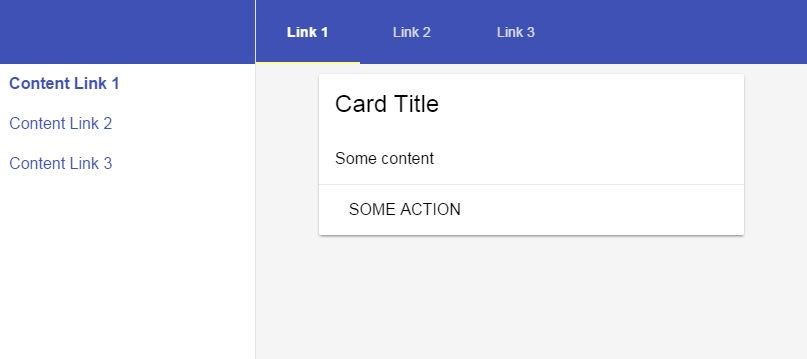
\includegraphics[width=12cm]{kapitel7/bilder/1-multi-navigation-app}
 \caption{Darstellung der multi-navigation-app-Komponente}
 \label{fig:ddmnak}
\end{figure}

Die Komponente steht unter Versionskontrolle und ist auf GitHub unter der Adresse \texttt{https://github.com/glur4k/multi-navigation-app} sowie im Anhang B zu finden. Sie kann nun mittels dem Tag \texttt{\textless{}multi-navigation-app\textgreater{}} auf allen Webseiten und Applikationen eingebunden werden.


\subsection{Deployment mit Bower}\label{deployment-mit-bower}

Um die Komponente für andere Entwickler verfügbar zu machen, damit diese sie einfach mit \texttt{bower\ install\ multi-navigation-app} installieren können, muss sie bei Bower registriert werden. Hierfür muss zunächst die \texttt{bower.json}-Datei um die korrekten Informationen ergänzt werden, da die Komponente sonst nicht von Bower indiziert werden kann. Entspricht die \texttt{bower.json} den Bower-Spezifikationen und wird auf GitHub gepusht, so wird die Komponente mittels dem Befehl \texttt{bower\ register\ multi-navigation-app\ git://github.com/glur4k/multi-navigation-app.git} bei Bower registriert. Sie ist somit unter der Adresse \texttt{http://bower.io/search/?q=multi-navigation-app} auf der Bower-Webseite zu finden. Mittels \texttt{bower\ info\ multi-navigation-app} kann die aktuelle Version der Komponente auf Bower ermittelt werden, welche dabei immer das aktuellste Release auf GitHub ist. Die Komponente kann nun von allen Entwicklern mittels Bower heruntergeladen und in die eigene Webseite oder Applikation eingebunden werden. Die \texttt{bower.json}-Datei ist zusätzlich um den Eintrag \texttt{\dq keywords\dq:\ {[}\ \dq web-components\dq\ {]}} erweitert, somit ist sie ebenso in dem customelements.io-Katalog unter der Adresse \texttt{https://customelements.io/glur4k/multi-navigation-app/} zu finden.

\section{Vergleich mit Komponenten-Entwicklung in AngularJS}\label{vergleich-mit-komponenten-entwicklung-in-angularjs}

Die mit Polymer in Abschnitt \ref{entwicklung-und-deployment-einer-polymer-komponente} implementierte Multi-Navigation-Application-Kom\-po\-nen\-te wird möglichst ähnlich mit AngularJS nachgebaut (siehe Anhang C und auf GitHub unter \texttt{https://github.com/glur4k/angular-multi-navigation-app}). In diesem Abschnitt werden die durch die beiden unterschiedlichen Implementierungen deutlich gewordenen Unterschiede zwischen Polymer und AngularJS dargestellt.


\subsection{Einstieg in AngularJS}\label{einstieg-in-angularjs}

AngularJS ist ein ebenfalls von Google entwickeltes, clientseitiges Open-Source-JavaScript-Framework zur Erstellung von dynamischen \ac{SPA}s. Ebenso wie Polymer erlaubt sie es, eigene \ac{HTML}-Elemente, unter AngularJS \texttt{Directives} genannt, zu erstellen, welche die native Sammlung an \ac{HTML}-Elementen erweitern können. Sie ist ein ``Fat-Client-Framework'', welches die gesamte Logik, sowie die View-Schicht auf dem Client hält und an ein serverseitiges, Daten-haltendes Model angebunden werden kann \cite{citeulike:13920434}. AngularJS verfolgt dabei den \ac{MVVM}-Ansatz, wie in Abbildung \ref{fig:ddmvvmavajs} dargestellt wird. Das \ac{MVVM}-Model stellt eine Erweiterung des \ac{MVC}-Ansatzes dar, wobei die Controller-Schicht durch eine ViewModel-Schicht ersetzt wird. Diese kann als eine Art Proxy aufgefasst werden, welche der View-Schicht nur die Daten des Models liefert, die sie tatsächlich benötigt. Hierbei kann die ViewModel-Schicht die Daten transformieren, damit sie von der View-Schicht ausgegeben werden können. Ebenso stellt sie die von der View-Schicht benötigten Funktionalitäten zum Ändern der Daten bereit.

\begin{figure}[htbp]
 \centering
 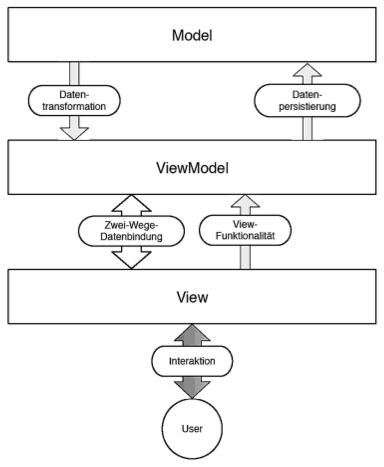
\includegraphics[width=8cm]{kapitel7/bilder/1-model-view-viewmodel}
 \caption{Darstellung der Model-View-ViewModel-Architektur von AngularJS}
 \label{fig:ddmvvmavajs}
\end{figure}

Zu den Kern-Konzepten von AngularJS gehören unter anderen das aus Polymer bekannte Two-Way-Data-Binding, die Controller sowie Direktiven. Das Two-Way-Data-Binding erlaubt die Datenbindung in zwei Richtungen, von Model zu View und umgekehrt. Die dabei entstehenden Änderungen am Model werden automatisch im \ac{DOM} abgebildet und Benutzerinteraktionen innerhalb des Views werden automatisch auf das Model angewendet. Dadurch entfällt die manuelle Manipulation des \ac{DOM}s mithilfe von JavaScript bzw. jQuery, da diese von AngularJS intern mittels der jQuery-lite, einer vereinfachten, leichteren Version von jQuery automatisch vollzogen wird. Die Controllers definieren die Daten und die Logik (ViewModel), die für einen bestimmten View benötigt werden. Sie halten hierfür einen Scope, in dem die Variablen und Funktionen definiert werden, auf die aus dem View heraus zugegriffen werden können soll. Soll mit Hilfe von AngularJS \ac{HTML} um eigene Elemente oder Attribute erweitert werden, so werden hierfür die Direktiven eingesetzt, welche die dafür notwendige Logik kapseln.


\subsection{Vergleich der Intentionen hinter Polymer und AngularJS}\label{vergleich-der-intentionen-hinter-polymer-und-angularjs}

Die Web Components sind eine Sammlung an sich noch in Entwicklung befindenden Technologien und APIs um eigene \ac{HTML}-Elemente zu definieren. Polymer ist eine Library um dies zu vereinfachen und erweitern. Mit Hilfe von Polyfills und zusätzlichen Features kann es \ac{HTML}-Elemente erstellen und sie auch auf Browsern zum Einsatz bringen, welche die nötigen Standards noch nicht unterstützen. AngularJS hingegen stellt APIs auf Framework-Ebene bereit wie Services, Routing oder auch Serverkommunikation. Die Polymer-Library bildet diese Funktionalitäten hingegen nicht ab. Stattdessen muss hierfür auf die mit Polymer entwickelten Iron Elements des Elemente Katalogs zurückgegriffen werden, da diese solche Funktionalitäten bieten. Es kümmert sich mehr darum, das Entwickeln solcher umfangreichen, mächtigen und wiederverwendbarer Komponenten zu ermöglichen. Mit diesen Komponenten wiederum können komplexe Applikationen realisiert werden, wie sie mit AngularJS umgesetzt werden können. Polymer muss daher als eine Library angesehen werden, wobei AngularJS ein komplettes Framework ist. Die durch Polymer erweiterten Web Components entsprechen vielmehr den Direktiven von Angular. Polymer ist also als ein Subset des AngularJS Funktionsumfangs, welcher für das Entwickeln von komplexen Applikationen entworfen ist, anzusehen.


\subsection{Vergleich der Technischen Features}\label{vergleich-der-technische-features}

Dennoch gibt es Features, die sowohl Polymer als auch AngularJS mitbringen. Hierzu zählt das Two-Way-Data-Binding mit einer sehr ähnlichen Syntax sowie die deklarativen Templates zum Definieren von Komponenten-internen Markups. Jedoch überwiegen die Unterschiede beider Funktionsumfänge.

AngularJS ist ein Framework zum Erstellen von \ac{SPA}s und stellt hierfür eine Reihe an Funktionalitäten bereit. Polymer hingegen bietet keine internen Mechanismen für das Strukturieren einer Applikation bereit, stattdessen können die hierfür mit Polymer entwickelten Komponenten eingesetzt werden. Eine mit Polymer realisierte Applikation ist dadurch deklarativ geschachtelt und hierarchisch aufgebaut, was durch das Mediator-Pattern erzwungen wird (siehe Abschnitt 5.1). AngularJS hingegen erfordert keine hierarchische Struktur, da es unter dem Framework nicht nur ein Typ von Komponenten gibt. Dies spiegelt sich auch in dessen Aufbau wieder, da die Definition von Elementen mit AngularJS imperativ in JavaScript erfolgt. Da Definition von Komponenten mit Polymer deklarativ orientiert ist, können diese auch einfacher mit anderen Komponenten, welche nicht mit Polymer erstellt werden, interagieren, da sie normales \ac{DOM} sind. AngularJS hingegen ist nur schwer mit anderen \ac{SPA}-Frameworks zu kombinieren. Des weiteren nutzt Polymer das Shadow \ac{DOM}, bzw. das Shady \ac{DOM}, um Stylesheets und JavaScripte in den Komponenten zu kapseln. In AngularJS wird hierauf verzichtet, da es nur die Daten in dem Scope kapselt. Auch ist das Deployment einer AngularJS-Direktiven einiges umständlicher als mit Polymer, da externe Templates immer relativ zum Projekt oder Domain-Root adressiert werden müssen. Hierzu ist ein zusätzlicher Build-Schritt nötig, der das Template in den Template-Cache schreibt, oder es in die Direktive serialisiert. Zuletzt ist die Browserunterstützung unter AngularJS deutlich breiter -- beispielsweise wird der Internet Explorer in Version 8 unterstützt -- wodurch es auch bei mehr Projekten in der Produktion eingesetzt werden kann.


\chapter{Zukunftsprognose}\label{zukunftsprognose}

Die Standards der Web-Component-Technologien sind noch nicht fertiggestellt und befinden sich momentan noch in Entwicklung. Um allgemeingültige Standards für alle Browserhersteller zu gewährleisten, werden sich diese vermutlich noch verändern. Jedoch werden sie dadurch ein breites Spektrum an Zustimmung und Implementierung bekommen, da sie eine zentrale Rolle spielen, wenn darum geht, auch das Web zu einer Plattform zu machen, für welche die Paradigmen von höheren Programmiersprachen gelten. So soll es auch im Web möglich sein, Applikationen aus mehreren verschiedenen Komponenten, die gekapselt, wartbar und interoperabel sind, zu entwickeln. Polymer wird dabei weiterhin eine wichtige Rolle innehaben, da die Bibliothek das Arbeiten mit den Web Components vereinfacht und zusätzliche Funktionalitäten dafür bereitstellt. Dabei könnte sogar ein Vergleich der Polymer Bibliothek und der jQuery Bibliothek vorstellbar sein. So wie jQuery zu einem De-Facto-Standard für das Arbeiten mit \ac{DOM}-Elementen wurde, so könnte Polymer ein Standard für das Arbeiten mit Web Components werden. Da Google maßgeblich die Entwicklung der Standards der Web Component Technologien vorantreibt und sich die anderen Browserhersteller teilweise daran orientieren, könnte es sogar sein, dass zumindest Teile von Polymer zum offiziellen Standard der Web Technologien wird.

Wenn die Standards von allen Browsern akzeptiert und implementiert wurden, sinkt auch die Komplexität von Polymer um ein Vielfaches, da die komplette Schicht der Polyfills wegfällt. Neben den Polyfills kann Polymer dann auf die Nutzung des Bibliothek-internen Shady \ac{DOM} verzichten und stattdessen mit einer standardisierten, schnellen und leichtgewichtigen Version des Shadow \ac{DOM} arbeiten. Dadurch wird Polymer um einiges schneller arbeiten und auch auf mobilen Geräten effizienten Einzug erhalten.

Neben Polymer basiert auch Angular ab Version 2.0 auf den Web-Component-Stan\-dards und wird dessen Technologien benutzen, jedoch verfolgt Angular einen anderen Ansatz als Polymer. Angular implementiert hierfür eine eigene Schicht, welche auf die nativen Technologien zugreift und das Framework komplexer macht. Da in Zukunft die Polyfills und der Shady \ac{DOM} der Polymer-Library wegfallen, könnte Angular Polymer in sich integrieren, statt die Web-Components-Standards selbst zu implementieren. Hierfür würde beispielsweise die Micro-Schicht in Frage kommen, da diese nur die Grundfunktionalitäten für den Umgang mit den Web Components leistet. Jedoch werden beide Bibliotheken weiterhin koexistieren und weder Polymer Angular ersetzen noch umgekehrt, da Polymer nur eine erweiterbare Library und Angular ein vollständiges Framework ist. Beide Plattformen verfolgen daher unterschiedliche Ansätze und können unterschiedliche Probleme lösen. Jedoch kann durch die Entwicklung der Carbon-Elemente die Polymer-Library sukzessive als Framework erweitert werden, da diese eine neue Möglichkeit bieten, wie Applikationen strukturiert werden können. Durch sie können komplexe Applikationen realisiert werden, da die Elemente sehr nah an der Plattform selbst sind, was einige Vorteile mit sich bringt. So haben sie wenige Abhängigkeiten, eine bessere Performance, können leicht ausgetauscht werden und bieten ein vereinfachtes Debugging an, da sie die Tools der Plattform statt die eines Frameworks benutzen. Polymer kann also als eine Library mit einem optionalen Framework-Plugin verstanden werden. Dieses bietet, je nach Anforderungen, Vor- und Nachteile wie jedes andere Framework auch. Es liegt somit weiterhin im Ermessen der Entwickler ob Angular oder Polymer eingesetzt werden soll, oder ob sogar -- bis zu einem gewissen Grad -- beides verwendet werden soll. Jedoch beschränkt sich Polymer nicht nur auf den Einsatz in Angular, sondern kann mit jedem beliebigem Framework kombiniert werden. Wie genau die Entwicklung von Polymer weiter verläuft und ob sich diese auf Angular auswirken wird, liegt jedoch ganz im Ermessen von Google.

Auch die Seitenbau GmbH beobachtet die Entwicklung der Web Components mit Interesse, jedoch können sie auch mittels Polymer momentan noch nicht produktiv eingesetzt werden. Die Ansprüche der Kunden bezüglich der zu unterstützenden Browser sind noch sehr hoch, so sollen in vielen Projekten noch ältere Versionen des Internet Explorers unterstützt werden, was weder Polymer noch dessen Polyfills gewährleisten. Auch ist die Performance insbesondere auf mobilen Browsern noch nicht ausreichend, so dass auf alternative Frameworks wie AngularJS zurückgegriffen wird. Sollten diese Rahmenbedienungen in Zukunft jedoch erfüllt werden, so könnte die Polymer-Library auch bei der Seitenbau GmbH einen produktiven Einzug erhalten.


\chapter*{Anhang A - Native Web Komponente}\label{anhang-a---native-web-komponente}
\addcontentsline{toc}{chapter}{Anhang A - Native Web Komponente}

\section*{HTML Struktur zum Benutzen einer Web Komponente mit den nativen APIs}\label{html-struktur-zum-benutzen-einer-web-komponente-mit-den-nativen-apis}

\textbf{index.html:}

\begin{Shaded}
\begin{Highlighting}[]
\DataTypeTok{<!DOCTYPE }\NormalTok{html}\DataTypeTok{>}
\KeywordTok{<html}\OtherTok{ lang=}\StringTok{"en"}\KeywordTok{>}
\KeywordTok{<head>}
  \KeywordTok{<meta}\OtherTok{ charset=}\StringTok{"UTF-8"}\KeywordTok{>}
  \KeywordTok{<title>}\NormalTok{Demo of a Custom Element}\KeywordTok{</title>}

  \CommentTok{<!-- Import the web component -->}
  \KeywordTok{<link}\OtherTok{ rel=}\StringTok{"import"}\OtherTok{ href=}\StringTok{"elements/custom-element.html"}\KeywordTok{>}
\KeywordTok{</head>}
\KeywordTok{<body>}

  \CommentTok{<!-- Use the web component -->}
  \KeywordTok{<custom-element}\OtherTok{ theme=}\StringTok{"style1"}\KeywordTok{>}\NormalTok{Reader}\KeywordTok{</custom-element>}

\KeywordTok{</body>}
\KeywordTok{</html>}
\end{Highlighting}
\end{Shaded}

\section*{Implementierung einer Web Komponente mit den nativen
APIs}\label{implementierung-einer-web-komponente-mit-den-nativen-apis}

\textbf{custom-element.html:}

\begin{Shaded}
\begin{Highlighting}[]
\KeywordTok{<template}\OtherTok{ id=}\StringTok{"myElementTemplate"}\KeywordTok{>}
  \KeywordTok{<style>}
    \FloatTok{.outer} \KeywordTok{\{} \ErrorTok{...} \KeywordTok{\}}
    \FloatTok{.style1} \KeywordTok{\{} \KeywordTok{color:} \DataTypeTok{green}\KeywordTok{;} \KeywordTok{\}}
    \FloatTok{.style2} \KeywordTok{\{} \KeywordTok{color:} \DataTypeTok{blue}\KeywordTok{;} \KeywordTok{\}}
    \FloatTok{.name} \KeywordTok{\{} \KeywordTok{font-size:} \DataTypeTok{35pt}\KeywordTok{;} \KeywordTok{padding-top:} \DataTypeTok{0.5em}\KeywordTok{;} \KeywordTok{\}}
  \KeywordTok{</style>}

  \KeywordTok{<div}\OtherTok{ class=}\StringTok{"outer"}\KeywordTok{>}
    \NormalTok{Welcome in the Web Component}
    \KeywordTok{<div}\OtherTok{ class=}\StringTok{"name"}\KeywordTok{>}
      \KeywordTok{<content></content>}
    \KeywordTok{</div>}
  \KeywordTok{</div>}
\KeywordTok{</template>}

\KeywordTok{<script>}
  \CommentTok{// Refers to the "importee", which is index.html}
  \KeywordTok{var} \NormalTok{importDoc }\OperatorTok{=} \VariableTok{document}\NormalTok{.}\VariableTok{currentScript}\NormalTok{.}\AttributeTok{ownerDocument}\OperatorTok{;}

  \CommentTok{// Creates an object based in the HTML Element prototype}
  \KeywordTok{var} \NormalTok{CustomElementProto }\OperatorTok{=} \VariableTok{Object}\NormalTok{.}\AttributeTok{create}\NormalTok{(}\VariableTok{HTMLElement}\NormalTok{.}\AttributeTok{prototype}\NormalTok{)}\OperatorTok{;}

  \CommentTok{// Creates the "theme" attribute and sets a default value}
  \VariableTok{CustomElementProto}\NormalTok{.}\AttributeTok{theme} \OperatorTok{=} \StringTok{'style1'}\OperatorTok{;}

  \CommentTok{// Fires when an instance of the element is created}
  \VariableTok{CustomElementProto}\NormalTok{.}\AttributeTok{createdCallback} \OperatorTok{=} \KeywordTok{function}\NormalTok{() }\OperatorTok{\{}

    \CommentTok{// Creates the shadow root}
    \KeywordTok{var} \NormalTok{shadow }\OperatorTok{=} \KeywordTok{this}\NormalTok{.}\AttributeTok{createShadowRoot}\NormalTok{()}\OperatorTok{;}

    \CommentTok{// Gets content from <template>}
    \KeywordTok{var} \NormalTok{template }\OperatorTok{=} \VariableTok{importDoc}\NormalTok{.}\AttributeTok{querySelector}\NormalTok{(}\StringTok{'#myElementTemplate'}\NormalTok{).}\AttributeTok{content}\OperatorTok{;}

    \CommentTok{// Adds a template clone into shadow root}
    \VariableTok{shadow}\NormalTok{.}\AttributeTok{appendChild}\NormalTok{(}\VariableTok{template}\NormalTok{.}\AttributeTok{cloneNode}\NormalTok{(}\KeywordTok{true}\NormalTok{))}\OperatorTok{;}

    \CommentTok{// Caches .outer DOM query}
    \KeywordTok{this}\NormalTok{.}\AttributeTok{outer} \OperatorTok{=} \VariableTok{shadow}\NormalTok{.}\AttributeTok{querySelector}\NormalTok{(}\StringTok{'.outer'}\NormalTok{)}\OperatorTok{;}

    \CommentTok{// Checks if the "theme" attribute has been overwritten}
    \ControlFlowTok{if} \NormalTok{(}\KeywordTok{this}\NormalTok{.}\AttributeTok{hasAttribute}\NormalTok{(}\StringTok{'theme'}\NormalTok{)) }\OperatorTok{\{}
      \KeywordTok{var} \NormalTok{theme }\OperatorTok{=} \KeywordTok{this}\NormalTok{.}\AttributeTok{getAttribute}\NormalTok{(}\StringTok{'theme'}\NormalTok{)}\OperatorTok{;}
      \KeywordTok{this}\NormalTok{.}\AttributeTok{setTheme}\NormalTok{(theme)}\OperatorTok{;}
    \OperatorTok{\}} \ControlFlowTok{else} \OperatorTok{\{}
      \KeywordTok{this}\NormalTok{.}\AttributeTok{setTheme}\NormalTok{(}\KeywordTok{this}\NormalTok{.}\AttributeTok{theme}\NormalTok{)}\OperatorTok{;}
    \OperatorTok{\}}
  \OperatorTok{\};}

  \CommentTok{// Fires when an attribute was added, removed, or updated}
  \VariableTok{CustomElementProto}\NormalTok{.}\AttributeTok{attributeChangedCallback} \OperatorTok{=} \KeywordTok{function}\NormalTok{(attr}\OperatorTok{,} \NormalTok{oldVal}\OperatorTok{,} \NormalTok{newVal) }\OperatorTok{\{}
    \ControlFlowTok{if} \NormalTok{(attr }\OperatorTok{===} \StringTok{'theme'}\NormalTok{) }\OperatorTok{\{}
      \KeywordTok{this}\NormalTok{.}\AttributeTok{setTheme}\NormalTok{(newVal)}\OperatorTok{;}
    \OperatorTok{\}}
  \OperatorTok{\};}

  \CommentTok{// Sets new value to "theme" attribute}
  \VariableTok{CustomElementProto}\NormalTok{.}\AttributeTok{setTheme} \OperatorTok{=} \KeywordTok{function}\NormalTok{(val) }\OperatorTok{\{}
    \KeywordTok{this}\NormalTok{.}\AttributeTok{theme} \OperatorTok{=} \NormalTok{val}\OperatorTok{;}
    \KeywordTok{this}\NormalTok{.}\VariableTok{outer}\NormalTok{.}\AttributeTok{className} \OperatorTok{=} \StringTok{"outer "} \OperatorTok{+} \KeywordTok{this}\NormalTok{.}\AttributeTok{theme}\OperatorTok{;}
  \OperatorTok{\};}

  \CommentTok{// Registers <custom-element> in the main document}
  \VariableTok{document}\NormalTok{.}\AttributeTok{registerElement}\NormalTok{(}\StringTok{"custom-element"}\OperatorTok{,} \OperatorTok{\{}
    \DataTypeTok{prototype}\OperatorTok{:} \NormalTok{CustomElementProto}
  \OperatorTok{\}}\NormalTok{)}\OperatorTok{;}
\KeywordTok{</script>}
\end{Highlighting}
\end{Shaded}


\chapter*{Anhang B -- Polymer Web Component}\label{anhang-b---polymer-web-component}
\addcontentsline{toc}{chapter}{Anhang B -- Polymer Web Component}

\section*{Polymer Seed-Element}\label{polymer-seed-element}

\textbf{my-element.html:}

\begin{Shaded}
\begin{Highlighting}[]
\KeywordTok{<link}\OtherTok{ rel=}\StringTok{"import"}\OtherTok{ href=}\StringTok{"../polymer/polymer.html"}\KeywordTok{>}

\CommentTok{<!--}
\CommentTok{An element providing a solution to no problem in particular.}

\CommentTok{Example:}

\CommentTok{    <my-element></my-element>}

\CommentTok{@group Seed Elements}
\CommentTok{@element my-element}
\CommentTok{@demo demo/index.html}
\CommentTok{@hero hero.svg}
\CommentTok{-->}
\KeywordTok{<dom-module}\OtherTok{ id=}\StringTok{"my-element"}\KeywordTok{>}

  \KeywordTok{<template>}
    \KeywordTok{<style>}
\ErrorTok{      :host \{}
        \NormalTok{display}\DecValTok{:} \NormalTok{block;}
        \NormalTok{box-sizing}\DecValTok{:} \NormalTok{border-box;}
      \NormalTok{\}}

      \FloatTok{.author} \NormalTok{img }\KeywordTok{\{}
        \KeywordTok{display:} \DataTypeTok{block}\KeywordTok{;}
        \KeywordTok{float:} \DataTypeTok{left}\KeywordTok{;}
        \KeywordTok{margin-right:} \DataTypeTok{5px}\KeywordTok{;}
        \KeywordTok{max-height:} \DataTypeTok{100px}\KeywordTok{;}
        \KeywordTok{max-width:} \DataTypeTok{100px}\KeywordTok{;}
      \KeywordTok{\}}
    \KeywordTok{</style>}
    \KeywordTok{<h1>}\DecValTok{&lt;}\NormalTok{my-element}\DecValTok{&gt;}\KeywordTok{</h1>}
    \KeywordTok{<content></content>}
    \KeywordTok{<p}\OtherTok{ class=}\StringTok{"author"}\KeywordTok{>}
      \KeywordTok{<img}\OtherTok{ src=}\StringTok{"\{\{author.image\}\}"}\KeywordTok{>}
      \NormalTok{Cheers,}\KeywordTok{<br/>}
      \KeywordTok{<span}\OtherTok{ class=}\StringTok{"name"}\KeywordTok{>}\NormalTok{\{\{author.name\}\}}\KeywordTok{</span>}
    \KeywordTok{</p>}
  \KeywordTok{</template>}

\KeywordTok{</dom-module>}

\KeywordTok{<script>}

  \AttributeTok{Polymer}\NormalTok{(}\OperatorTok{\{}

    \DataTypeTok{is}\OperatorTok{:} \StringTok{'my-element'}\OperatorTok{,}

    \DataTypeTok{properties}\OperatorTok{:} \OperatorTok{\{}

      \CommentTok{/**}
\CommentTok{       * `fancy` indicates that the element should don a monocle and tophat,}
\CommentTok{       * while checking its pocket watch.}
\CommentTok{       */}
      \DataTypeTok{fancy}\OperatorTok{:} \NormalTok{Boolean}\OperatorTok{,}

      \CommentTok{/**}
\CommentTok{       * Describes the author of the element, but is really just an excuse to}
\CommentTok{       * show off JSDoc annotations.}
\CommentTok{       *}
\CommentTok{       * }\NormalTok{@type}\CommentTok{ \{\{name: string, image: string\}\}}
\CommentTok{       */}
      \DataTypeTok{author}\OperatorTok{:} \OperatorTok{\{}
        \DataTypeTok{type}\OperatorTok{:} \NormalTok{Object}\OperatorTok{,}
        \CommentTok{// Use `value` to provide a default value for a property, by setting it}
        \CommentTok{// on your element's prototype.}
        \CommentTok{//}
        \CommentTok{// If you provide a function, as we do here, Polymer will call that}
        \CommentTok{// _per element instance_.}
        \CommentTok{//}
        \CommentTok{// We do that to ensure that each element gets its own copy of the}
        \CommentTok{// value, rather than having it shared across all instances (via the}
        \CommentTok{// prototype).}
        \DataTypeTok{value}\OperatorTok{:} \KeywordTok{function}\NormalTok{() }\OperatorTok{\{}
          \ControlFlowTok{return} \OperatorTok{\{}
            \DataTypeTok{name}\OperatorTok{:}  \StringTok{'Dimitri Glazkov'}\OperatorTok{,}
            \DataTypeTok{image}\OperatorTok{:} \StringTok{'http://addyosmani.com/unicorn.jpg'}\OperatorTok{,}
          \OperatorTok{\};}
        \OperatorTok{\}}
      \OperatorTok{\},}

    \OperatorTok{\},}

    \CommentTok{// Element Lifecycle}

    \DataTypeTok{ready}\OperatorTok{:} \KeywordTok{function}\NormalTok{() }\OperatorTok{\{}
      \CommentTok{// `ready` is called after all elements have been configured, but}
      \CommentTok{// propagates bottom-up. This element's children are ready, but parents}
      \CommentTok{// are not.}
      \CommentTok{//}
      \CommentTok{// This is the point where you should make modifications to the DOM (when}
      \CommentTok{// necessary), or kick off any processes the element wants to perform.}
    \OperatorTok{\},}

    \DataTypeTok{attached}\OperatorTok{:} \KeywordTok{function}\NormalTok{() }\OperatorTok{\{}
      \CommentTok{// `attached` fires once the element and its parents have been inserted}
      \CommentTok{// into a document.}
      \CommentTok{//}
      \CommentTok{// This is a good place to perform any work related to your element's}
      \CommentTok{// visual state or active behavior (measuring sizes, beginning animations,}
      \CommentTok{// loading resources, etc).}
    \OperatorTok{\},}

    \DataTypeTok{detached}\OperatorTok{:} \KeywordTok{function}\NormalTok{() }\OperatorTok{\{}
      \CommentTok{// The analog to `attached`, `detached` fires when the element has been}
      \CommentTok{// removed from a document.}
      \CommentTok{//}
      \CommentTok{// Use this to clean up anything you did in `attached`.}
    \OperatorTok{\},}

    \CommentTok{// Element Behavior}

    \CommentTok{/**}
\CommentTok{     * The `my-element-lasers` event is fired whenever `fireLasers` is called.}
\CommentTok{     *}
\CommentTok{     * }\NormalTok{@event}\CommentTok{ my-element-lasers}
\CommentTok{     * }\NormalTok{@detail}\CommentTok{ \{\{sound: String\}\}}
\CommentTok{     */}

    \CommentTok{/**}
\CommentTok{     * Sometimes it's just nice to say hi.}
\CommentTok{     *}
\CommentTok{     * }\KeywordTok{@param}\CommentTok{ }\KeywordTok{\{string\}}\CommentTok{ greeting A positive greeting.}
\CommentTok{     * }\KeywordTok{@return}\CommentTok{ \{string\} The full greeting.}
\CommentTok{     */}
    \DataTypeTok{sayHello}\OperatorTok{:} \KeywordTok{function}\NormalTok{(greeting) }\OperatorTok{\{}
      \KeywordTok{var} \NormalTok{response }\OperatorTok{=} \NormalTok{greeting }\OperatorTok{||} \StringTok{'Hello World!'}\OperatorTok{;}
      \ControlFlowTok{return} \StringTok{'my-element says, '} \OperatorTok{+} \NormalTok{response}\OperatorTok{;}
    \OperatorTok{\},}

    \CommentTok{/**}
\CommentTok{     * Attempt to destroy this element's enemies with a beam of light!}
\CommentTok{     *}
\CommentTok{     * Or, at least, dispatch an event in the vain hope that someone else will}
\CommentTok{     * do the zapping.}
\CommentTok{     */}
    \DataTypeTok{fireLasers}\OperatorTok{:} \KeywordTok{function}\NormalTok{() }\OperatorTok{\{}
      \KeywordTok{this}\NormalTok{.}\AttributeTok{fire}\NormalTok{(}\StringTok{'my-element-lasers'}\OperatorTok{,} \OperatorTok{\{}\DataTypeTok{sound}\OperatorTok{:} \StringTok{'Pew pew!'}\OperatorTok{\}}\NormalTok{)}\OperatorTok{;}
    \OperatorTok{\}}

  \OperatorTok{\}}\NormalTok{)}\OperatorTok{;}

\KeywordTok{</script>}
\end{Highlighting}
\end{Shaded}

\newpage
\section*{Implementierung der Polymer Komponente Multi-Navigation-App}\label{implementierung-der-polymer-Komponente-multi-navigation-app}

\textbf{multi-navigation-app.html:}

\begin{Shaded}
\begin{Highlighting}[]

\KeywordTok{<link}\OtherTok{ rel=}\StringTok{"import"}\OtherTok{ href=}\StringTok{"../paper-tabs/paper-tabs.html"}\KeywordTok{>}
\KeywordTok{<link}\OtherTok{ rel=}\StringTok{"import"}\OtherTok{ href=}\StringTok{"../paper-toolbar/paper-toolbar.html"}\KeywordTok{>}
\KeywordTok{<link}\OtherTok{ rel=}\StringTok{"import"}\OtherTok{ href=}\StringTok{"../iron-pages/iron-pages.html"}\KeywordTok{>}
\KeywordTok{<link}\OtherTok{ rel=}\StringTok{"import"}\OtherTok{ href=}\StringTok{"../paper-drawer-panel/paper-drawer-panel.html"}\KeywordTok{>}
\KeywordTok{<link}\OtherTok{ rel=}\StringTok{"import"}\OtherTok{ href=}\StringTok{"../paper-button/paper-button.html"}\KeywordTok{>}
\KeywordTok{<link}\OtherTok{ rel=}\StringTok{"import"}\OtherTok{ href=}\StringTok{"../paper-icon-button/paper-icon-button.html"}\KeywordTok{>}
\KeywordTok{<link}\OtherTok{ rel=}\StringTok{"import"}\OtherTok{ href=}\StringTok{"../paper-card/paper-card.html"}\KeywordTok{>}
\KeywordTok{<link}\OtherTok{ rel=}\StringTok{"import"}\OtherTok{ href=}\StringTok{"../iron-icons/iron-icons.html"}\KeywordTok{>}

\KeywordTok{<dom-module}\OtherTok{ id=}\StringTok{"multi-navigation-app"}\KeywordTok{>}
  \KeywordTok{<template>}
    \KeywordTok{<style>}
\ErrorTok{      :host \{}
        \NormalTok{display}\DecValTok{:} \NormalTok{block;}
        \NormalTok{box-sizing}\DecValTok{:} \NormalTok{border-box;}
      \NormalTok{\}}
      \NormalTok{paper-tabs }\KeywordTok{\{}
        \KeywordTok{color:} \DataTypeTok{#fff}\KeywordTok{;}
        \KeywordTok{height:} \DataTypeTok{100%}\KeywordTok{;}
        \KeywordTok{margin:} \DataTypeTok{auto} \DataTypeTok{-16px}\KeywordTok{;}
      \KeywordTok{\}}
\ErrorTok{      #topnavi ::content paper-tab \{}
        \NormalTok{min-width}\DecValTok{:} \NormalTok{50px;}
      \NormalTok{\}}
      \DecValTok{@media} \DecValTok{only all and (min-width: }\DataTypeTok{600px}\DecValTok{) \{}
        \FloatTok{#topnavi} \DecValTok{::}\NormalTok{content paper-tab }\KeywordTok{\{}
          \KeywordTok{min-width:} \DataTypeTok{80px}\KeywordTok{;}
        \KeywordTok{\}}
      \DecValTok{\}}
\ErrorTok{      #leftnavi ::content paper-button \{}
        \NormalTok{margin}\DecValTok{:} \NormalTok{0;}
        \NormalTok{width}\DecValTok{:} \NormalTok{100%;}
        \NormalTok{text-align}\DecValTok{:} \NormalTok{left;}
        \NormalTok{color}\DecValTok{:} \NormalTok{#3f51b5;}
        \NormalTok{text-transform}\DecValTok{:} \NormalTok{none;}
      \NormalTok{\}}
\ErrorTok{      #leftnavi ::content paper-button.iron-selected \{}
        \NormalTok{font-weight}\DecValTok{:} \NormalTok{bold;}
      \NormalTok{\}}
      \NormalTok{iron-pages }\KeywordTok{\{}
        \KeywordTok{position:} \DataTypeTok{relative}\KeywordTok{;}
      \KeywordTok{\}}
      \FloatTok{#paperDrawerPanel} \CharTok{[drawer]}\DecValTok{:not}\NormalTok{(}\CharTok{[style-scope]}\NormalTok{)}\DecValTok{:not}\NormalTok{(}\FloatTok{.style-scope}\NormalTok{) }\KeywordTok{\{}
        \KeywordTok{border-right:} \DataTypeTok{1px} \DataTypeTok{solid} \DataTypeTok{#e0e0e0}\KeywordTok{;}
      \KeywordTok{\}}
      \NormalTok{paper-drawer-panel }\KeywordTok{\{}
        \KeywordTok{--paper-drawer-panel-main-container:} \NormalTok{\{}
          \NormalTok{background-color: }\DataTypeTok{#f5f5f5}\KeywordTok{;}
        \KeywordTok{\}}\NormalTok{;}
        \NormalTok{--paper-drawer-panel-left-drawer-container}\DecValTok{:} \KeywordTok{\{}
          \KeywordTok{border-right:} \DataTypeTok{1px} \DataTypeTok{solid} \DataTypeTok{#e5e5e5}\KeywordTok{;}
        \KeywordTok{\}}\NormalTok{;}
      \NormalTok{\}}
\ErrorTok{      #contents ::content paper-card \{}
        \NormalTok{margin}\DecValTok{:} \NormalTok{0 10%;}
        \NormalTok{width}\DecValTok{:} \NormalTok{80%;}
      \NormalTok{\}}
    \KeywordTok{</style>}

    \KeywordTok{<paper-drawer-panel>}
      \KeywordTok{<paper-header-panel}\OtherTok{ drawer}\KeywordTok{>}
        \KeywordTok{<paper-toolbar></paper-toolbar>}

        \CommentTok{<!-- Left Navigation -->}
        \KeywordTok{<iron-pages}\OtherTok{ id=}\StringTok{"leftnavi"}\KeywordTok{>}
          \KeywordTok{<content}\OtherTok{ select=}\StringTok{"iron-selector"}\KeywordTok{></content>}
        \KeywordTok{</iron-pages>}
      \KeywordTok{</paper-header-panel>}

      \KeywordTok{<paper-header-panel}\OtherTok{ main}\KeywordTok{>}
        \KeywordTok{<paper-toolbar>}
          \KeywordTok{<paper-icon-button}\OtherTok{ icon=}\StringTok{"menu"}\OtherTok{ paper-drawer-toggle}\KeywordTok{>}
          \KeywordTok{</paper-icon-button>}

          \CommentTok{<!-- Top Navigation -->}
          \KeywordTok{<paper-tabs}\OtherTok{ id=}\StringTok{"topnavi"}\OtherTok{ selected=}\StringTok{"\{\{selectedTop\}\}"}\KeywordTok{>}
            \KeywordTok{<content}\OtherTok{ select=}\StringTok{"paper-tab"}\KeywordTok{></content>}
          \KeywordTok{</paper-tabs>}
        \KeywordTok{</paper-toolbar>}

        \CommentTok{<!-- Main Content -->}
        \KeywordTok{<iron-pages}\OtherTok{ id=}\StringTok{"contents"}\OtherTok{ selected=}\StringTok{"\{\{selectedContent\}\}"}\KeywordTok{>}
          \KeywordTok{<content}\OtherTok{ select=}\StringTok{".main"}\KeywordTok{></content>}
        \KeywordTok{</iron-pages>}
      \KeywordTok{</paper-header-panel>}
    \KeywordTok{</paper-drawer-panel>}

  \KeywordTok{</template>}
\KeywordTok{</dom-module>}

\KeywordTok{<script>}
  \AttributeTok{Polymer}\NormalTok{(}\OperatorTok{\{}
    \DataTypeTok{is}\OperatorTok{:} \StringTok{'multi-navigation-app'}\OperatorTok{,}

    \DataTypeTok{properties}\OperatorTok{:} \OperatorTok{\{}
      \DataTypeTok{selectedTop}\OperatorTok{:} \OperatorTok{\{}
        \DataTypeTok{type}\OperatorTok{:} \NormalTok{Number}\OperatorTok{,}
        \DataTypeTok{value}\OperatorTok{:} \DecValTok{0}
      \OperatorTok{\},}
      \DataTypeTok{selectedContent}\OperatorTok{:} \OperatorTok{\{}
        \DataTypeTok{type}\OperatorTok{:} \NormalTok{Number}\OperatorTok{,}
        \DataTypeTok{value}\OperatorTok{:} \DecValTok{0}
      \OperatorTok{\}}
    \OperatorTok{\},}

    \CommentTok{// Element Behavior}
    \DataTypeTok{_countLinks}\OperatorTok{:} \KeywordTok{function}\NormalTok{() }\OperatorTok{\{}
      \KeywordTok{var} \NormalTok{count }\OperatorTok{=} \DecValTok{0}\OperatorTok{;}
      \KeywordTok{this}\NormalTok{.}\VariableTok{$}\NormalTok{.}\VariableTok{leftnavi}\NormalTok{.}\AttributeTok{getContentChildren}\NormalTok{().}\AttributeTok{forEach}\NormalTok{(}\KeywordTok{function} \NormalTok{(value}\OperatorTok{,} \NormalTok{i) }\OperatorTok{\{}
        \KeywordTok{var} \NormalTok{links }\OperatorTok{=} \VariableTok{value}\NormalTok{.}\AttributeTok{children}\OperatorTok{;}
        \ControlFlowTok{for} \NormalTok{(j }\OperatorTok{=} \DecValTok{0}\OperatorTok{;} \NormalTok{j }\OperatorTok{<} \VariableTok{links}\NormalTok{.}\AttributeTok{length}\OperatorTok{;} \NormalTok{j}\OperatorTok{++}\NormalTok{) }\OperatorTok{\{}
          \NormalTok{count}\OperatorTok{++;}
          \NormalTok{links[j].}\AttributeTok{linkNum} \OperatorTok{=} \NormalTok{(count }\OperatorTok{-} \DecValTok{1}\NormalTok{)}\OperatorTok{;}
        \OperatorTok{\}}
      \OperatorTok{\}}\NormalTok{)}\OperatorTok{;}
    \OperatorTok{\},}

    \NormalTok{_getSelectedContent}\OperatorTok{:} \KeywordTok{function}\NormalTok{() }\OperatorTok{\{}
      \ControlFlowTok{return} \KeywordTok{this}\NormalTok{.}\VariableTok{$}\NormalTok{.}\VariableTok{leftnavi}\NormalTok{.}\AttributeTok{getContentChildren}\NormalTok{()[}\KeywordTok{this}\NormalTok{.}\VariableTok{$}\NormalTok{.}\VariableTok{topnavi}\NormalTok{.}\AttributeTok{selected}\NormalTok{]}
        \NormalTok{.}\VariableTok{selectedItem}\NormalTok{.}\AttributeTok{linkNum}\OperatorTok{;}
    \OperatorTok{\},}

    \NormalTok{_addSelectedHandler}\OperatorTok{:} \KeywordTok{function}\NormalTok{() }\OperatorTok{\{}
      \KeywordTok{var} \NormalTok{topNaviItems }\OperatorTok{=} \KeywordTok{this}\NormalTok{.}\VariableTok{$}\NormalTok{.}\AttributeTok{topnavi}\OperatorTok{;}
      \KeywordTok{var} \NormalTok{leftNaviItems }\OperatorTok{=} \KeywordTok{this}\NormalTok{.}\VariableTok{$}\NormalTok{.}\AttributeTok{leftnavi}\OperatorTok{;}
      \KeywordTok{var} \NormalTok{contents }\OperatorTok{=} \KeywordTok{this}\NormalTok{.}\VariableTok{$}\NormalTok{.}\AttributeTok{contents}\OperatorTok{;}
      \KeywordTok{var} \NormalTok{that }\OperatorTok{=} \KeywordTok{this}\OperatorTok{;}

      \VariableTok{topNaviItems}\NormalTok{.}\AttributeTok{addEventListener}\NormalTok{(}\StringTok{'iron-select'}\OperatorTok{,} \KeywordTok{function}\NormalTok{() }\OperatorTok{\{}
        \CommentTok{// init first selected}
        \VariableTok{leftNaviItems}\NormalTok{.}\AttributeTok{select}\NormalTok{(}\VariableTok{that}\NormalTok{.}\AttributeTok{selectedTop}\NormalTok{)}\OperatorTok{;}
        \KeywordTok{var} \NormalTok{leftSelected }\OperatorTok{=} \VariableTok{leftNaviItems}\NormalTok{.}\AttributeTok{getContentChildren}\NormalTok{()[that}
          \NormalTok{.}\AttributeTok{selectedTop}\NormalTok{].}\AttributeTok{selectedItem}\OperatorTok{;}
        \ControlFlowTok{if} \NormalTok{(}\KeywordTok{typeof} \NormalTok{leftSelected }\OperatorTok{==} \StringTok{'undefined'}\NormalTok{) }\OperatorTok{\{}
          \VariableTok{leftNaviItems}\NormalTok{.}\AttributeTok{getContentChildren}\NormalTok{()[}\VariableTok{that}\NormalTok{.}\AttributeTok{selectedTop}\NormalTok{].}\AttributeTok{select}\NormalTok{(}\DecValTok{0}\NormalTok{)}
        \OperatorTok{\}}

        \VariableTok{contents}\NormalTok{.}\AttributeTok{select}\NormalTok{(}\VariableTok{that}\NormalTok{.}\AttributeTok{_getSelectedContent}\NormalTok{())}\OperatorTok{;}
      \OperatorTok{\}}\NormalTok{)}\OperatorTok{;}

      \VariableTok{leftNaviItems}\NormalTok{.}\AttributeTok{getContentChildren}\NormalTok{().}\AttributeTok{forEach}\NormalTok{(}\KeywordTok{function} \NormalTok{(value}\OperatorTok{,} \NormalTok{i) }\OperatorTok{\{}
        \VariableTok{value}\NormalTok{.}\AttributeTok{addEventListener}\NormalTok{(}\StringTok{'iron-select'}\OperatorTok{,} \KeywordTok{function} \NormalTok{(e) }\OperatorTok{\{}
          \VariableTok{contents}\NormalTok{.}\AttributeTok{select}\NormalTok{(}\VariableTok{that}\NormalTok{.}\AttributeTok{_getSelectedContent}\NormalTok{())}\OperatorTok{;}
        \OperatorTok{\}}\NormalTok{)}\OperatorTok{;}
      \OperatorTok{\}}\NormalTok{)}\OperatorTok{;}
    \OperatorTok{\},}
  \OperatorTok{\}}\NormalTok{)}\OperatorTok{;}
\KeywordTok{</script>}
\end{Highlighting}
\end{Shaded}

\chapter*{Anhang C -- AngularJS-Direktive}\label{anhang-c---angularjs-web-component}
\addcontentsline{toc}{chapter}{Anhang C -- AngularJS-Direktive}

\section*{Controller der AnngularJS-Applikation angular-multi-navigation-application}\label{controller-der-angular-multi-navigation-application}

\textbf{main.js:}

\begin{Shaded}
\begin{Highlighting}[]
\StringTok{'use strict'}\OperatorTok{;}

\CommentTok{/**}
\CommentTok{ * }\NormalTok{@ngdoc}\CommentTok{ function}
\CommentTok{ * }\KeywordTok{@name}\CommentTok{ }\StringTok{multiNavigationApp.controller:MainCtrl}
\CommentTok{ * }\NormalTok{@description}
\CommentTok{ * # MainCtrl}
\CommentTok{ * Controller of the multiNavigationApp}
\CommentTok{ */}
\VariableTok{angular}\NormalTok{.}\AttributeTok{module}\NormalTok{(}\StringTok{'multiNavigationApp'}\NormalTok{)}
  \NormalTok{.}\AttributeTok{controller}\NormalTok{(}\StringTok{'MainCtrl'}\OperatorTok{,} \KeywordTok{function} \NormalTok{($scope) }\OperatorTok{\{}
    \VariableTok{$scope}\NormalTok{.}\AttributeTok{sections} \OperatorTok{=} \NormalTok{[}\OperatorTok{\{}
      \DataTypeTok{title}\OperatorTok{:} \StringTok{'Nav 1'}\OperatorTok{,}
      \DataTypeTok{subSections}\OperatorTok{:} \NormalTok{[}\OperatorTok{\{}
        \DataTypeTok{title}\OperatorTok{:} \StringTok{'Sub-Nav 1.1'}\OperatorTok{,}
        \DataTypeTok{content}\OperatorTok{:} \StringTok{'Content 1.1'}
      \OperatorTok{\},} \OperatorTok{\{}
        \DataTypeTok{title}\OperatorTok{:} \StringTok{'Sub-Nav 1.2'}\OperatorTok{,}
        \DataTypeTok{content}\OperatorTok{:} \StringTok{'Content 1.2'}
      \OperatorTok{\},} \OperatorTok{\{}
        \DataTypeTok{title}\OperatorTok{:} \StringTok{'Sub-Nav 1.3'}\OperatorTok{,}
        \DataTypeTok{content}\OperatorTok{:} \StringTok{'Content 1.3'}
      \OperatorTok{\},} \OperatorTok{\{}
        \DataTypeTok{title}\OperatorTok{:} \StringTok{'Sub-Nav 1.4'}\OperatorTok{,}
        \DataTypeTok{content}\OperatorTok{:} \StringTok{'Content 1.4'}
      \OperatorTok{\}}\NormalTok{]}
    \OperatorTok{\},} \OperatorTok{\{}
      \DataTypeTok{title}\OperatorTok{:} \StringTok{'Nav 2'}\OperatorTok{,}
      \DataTypeTok{subSections}\OperatorTok{:} \NormalTok{[}\OperatorTok{\{}
        \DataTypeTok{title}\OperatorTok{:} \StringTok{'Sub-Nav 2.1'}\OperatorTok{,}
        \DataTypeTok{content}\OperatorTok{:} \StringTok{'Content 2.1'}
      \OperatorTok{\},} \OperatorTok{\{}
        \DataTypeTok{title}\OperatorTok{:} \StringTok{'Sub-Nav 2.2'}\OperatorTok{,}
        \DataTypeTok{content}\OperatorTok{:} \StringTok{'Content 2.2'}
      \OperatorTok{\},} \OperatorTok{\{}
        \DataTypeTok{title}\OperatorTok{:} \StringTok{'Sub-Nav 2.3'}\OperatorTok{,}
        \DataTypeTok{content}\OperatorTok{:} \StringTok{'Content 2.3'}
      \OperatorTok{\},} \OperatorTok{\{}
        \DataTypeTok{title}\OperatorTok{:} \StringTok{'Sub-Nav 2.4'}\OperatorTok{,}
        \DataTypeTok{content}\OperatorTok{:} \StringTok{'Content 2.4'}
      \OperatorTok{\}}\NormalTok{]}
    \OperatorTok{\},} \OperatorTok{\{}
      \DataTypeTok{title}\OperatorTok{:} \StringTok{'Nav 3'}\OperatorTok{,}
      \DataTypeTok{subSections}\OperatorTok{:} \NormalTok{[}\OperatorTok{\{}
        \DataTypeTok{title}\OperatorTok{:} \StringTok{'Sub-Nav 3.1'}\OperatorTok{,}
        \DataTypeTok{content}\OperatorTok{:} \StringTok{'Content 3.1'}
      \OperatorTok{\},} \OperatorTok{\{}
        \DataTypeTok{title}\OperatorTok{:} \StringTok{'Sub-Nav 3.2'}\OperatorTok{,}
        \DataTypeTok{content}\OperatorTok{:} \StringTok{'Content 3.2'}
      \OperatorTok{\},} \OperatorTok{\{}
        \DataTypeTok{title}\OperatorTok{:} \StringTok{'Sub-Nav 3.3'}\OperatorTok{,}
        \DataTypeTok{content}\OperatorTok{:} \StringTok{'Content 3.3'}
      \OperatorTok{\},} \OperatorTok{\{}
        \DataTypeTok{title}\OperatorTok{:} \StringTok{'Sub-Nav 3.4'}\OperatorTok{,}
        \DataTypeTok{content}\OperatorTok{:} \StringTok{'Content 3.4'}
      \OperatorTok{\}}\NormalTok{]}
    \OperatorTok{\}}\NormalTok{]}\OperatorTok{;}
  \OperatorTok{\}}\NormalTok{)}\OperatorTok{;}
\end{Highlighting}
\end{Shaded}

\section*{Direktive der AnngularJS-Applikation angular-multi-navigation-application}\label{direktive-der-angular-multi-navigation-application}

\textbf{multi-navigation.js:}

\begin{Shaded}
\begin{Highlighting}[]
\StringTok{'use strict'}\OperatorTok{;}

\CommentTok{/**}
\CommentTok{ * }\NormalTok{@ngdoc}\CommentTok{ directive}
\CommentTok{ * }\KeywordTok{@name}\CommentTok{ }\StringTok{multiNavigationApp.directive:multiNavigation}
\CommentTok{ * }\NormalTok{@description}
\CommentTok{ * # multiNavigation}
\CommentTok{ */}
\VariableTok{angular}\NormalTok{.}\AttributeTok{module}\NormalTok{(}\StringTok{'multiNavigationApp'}\NormalTok{)}
  \NormalTok{.}\AttributeTok{directive}\NormalTok{(}\StringTok{'multiNavigation'}\OperatorTok{,} \KeywordTok{function} \NormalTok{() }\OperatorTok{\{}
    \ControlFlowTok{return} \OperatorTok{\{}
      \DataTypeTok{scope}\OperatorTok{:} \OperatorTok{\{}
        \DataTypeTok{sections}\OperatorTok{:} \StringTok{'='}
      \OperatorTok{\},}
      \DataTypeTok{link}\OperatorTok{:} \KeywordTok{function} \NormalTok{($scope) }\OperatorTok{\{}
        \VariableTok{$scope}\NormalTok{.}\AttributeTok{selectSection} \OperatorTok{=} \KeywordTok{function} \NormalTok{(section) }\OperatorTok{\{}
          \VariableTok{$scope}\NormalTok{.}\AttributeTok{selectedSection} \OperatorTok{=} \NormalTok{section}\OperatorTok{;}
          \VariableTok{$scope}\NormalTok{.}\AttributeTok{selectedSubSection} \OperatorTok{=} \VariableTok{section}\NormalTok{.}\AttributeTok{lastSelected} \OperatorTok{||}
            \VariableTok{section}\NormalTok{.}\AttributeTok{subSections}\NormalTok{[}\DecValTok{0}\NormalTok{]}\OperatorTok{;}
        \OperatorTok{\};}
        \VariableTok{$scope}\NormalTok{.}\AttributeTok{selectSubSection} \OperatorTok{=} \KeywordTok{function} \NormalTok{(subSection) }\OperatorTok{\{}
          \VariableTok{$scope}\NormalTok{.}\AttributeTok{selectedSubSection} \OperatorTok{=} \NormalTok{subSection}\OperatorTok{;}
          \VariableTok{$scope}\NormalTok{.}\VariableTok{selectedSection}\NormalTok{.}\AttributeTok{lastSelected} \OperatorTok{=} \NormalTok{subSection}\OperatorTok{;}
        \OperatorTok{\};}
        \VariableTok{$scope}\NormalTok{.}\AttributeTok{selectedSection} \OperatorTok{=} \VariableTok{$scope}\NormalTok{.}\AttributeTok{sections}\NormalTok{[}\DecValTok{0}\NormalTok{]}\OperatorTok{;}
        \VariableTok{$scope}\NormalTok{.}\AttributeTok{selectedSubSection} \OperatorTok{=} \VariableTok{$scope}\NormalTok{.}\VariableTok{selectedSection}\NormalTok{.}\AttributeTok{subSections}\NormalTok{[}\DecValTok{0}\NormalTok{]}\OperatorTok{;}
      \OperatorTok{\},}
      \DataTypeTok{templateUrl}\OperatorTok{:} \StringTok{'views/multi-navigation.html'}
    \OperatorTok{\};}
  \OperatorTok{\}}\NormalTok{)}\OperatorTok{;}
\end{Highlighting}
\end{Shaded}

\section*{View des Controllers der AnngularJS-Applikation angular-multi-navigation-application}\label{view-des-controllers-der-angular-multi-navigation-application}

\textbf{main.html:}

\begin{Shaded}
\begin{Highlighting}[]
\KeywordTok{<div}\OtherTok{ layout=}\StringTok{"column"}\OtherTok{ layout-fill}\KeywordTok{>}
  \KeywordTok{<md-toolbar}\OtherTok{ class=}\StringTok{"md-hue-3"}\KeywordTok{>}
    \KeywordTok{<div}\OtherTok{ class=}\StringTok{"md-toolbar-tools"}\KeywordTok{>}
      \KeywordTok{<span>}\NormalTok{multi-navigation-app angular}\KeywordTok{</span>}
      \CommentTok{<!-- fill up the space between left and right area -->}
      \KeywordTok{<span}\OtherTok{ flex}\KeywordTok{></span>}
    \KeywordTok{</div>}
  \KeywordTok{</md-toolbar>}
  \KeywordTok{<md-content>}
      \KeywordTok{<multi-navigation}\OtherTok{ sections=}\StringTok{"sections"}\KeywordTok{></multi-navigation>}
  \KeywordTok{</md-content>}
\KeywordTok{</div>}
\end{Highlighting}
\end{Shaded}

\section*{View der Direktive der AnngularJS-Applikation angular-multi-navigation-application}\label{view-der-direktive-der-angular-multi-navigation-application}

\textbf{multi-navigation.html:}

\begin{Shaded}
\begin{Highlighting}[]
\KeywordTok{<div}\OtherTok{ layout=}\StringTok{"row"}\KeywordTok{>}
  \KeywordTok{<md-sidenav}\OtherTok{ md-component-id=}\StringTok{"left"}\OtherTok{ md-is-locked-open=}\StringTok{"true"}
\OtherTok{    class=}\StringTok{"md-sidenav-left"}\KeywordTok{>}
    \KeywordTok{<md-toolbar></md-toolbar>}
    \KeywordTok{<md-content}\OtherTok{ layout-padding}\KeywordTok{>}
      \KeywordTok{<md-list}\OtherTok{ ng-if=}\StringTok{"selectedSection"}\KeywordTok{>}
        \KeywordTok{<md-list-item}
\OtherTok{          ng-repeat=}\StringTok{"subSection in selectedSection.subSections"}
\OtherTok{          ng-click=}\StringTok{"selectSubSection(subSection)"}
\OtherTok{          ng-class=}\StringTok{"\{'selected' : selectedSubSection === subSection\}"}\KeywordTok{>}
          \NormalTok{\{\{subSection.title\}\}}
        \KeywordTok{</md-list-item>}
      \KeywordTok{</md-list>}
    \KeywordTok{</md-content>}
  \KeywordTok{</md-sidenav>}
  \KeywordTok{<div}\OtherTok{ flex}\KeywordTok{>}
    \KeywordTok{<md-toolbar>}
      \KeywordTok{<md-tabs}\OtherTok{ md-selected=}\StringTok{"0"}\OtherTok{ md-border-bottom md-no-pagination}\KeywordTok{>}
        \KeywordTok{<md-tab}
\OtherTok{          ng-click=}\StringTok{"selectSection(section)"}
\OtherTok{          ng-repeat=}\StringTok{"section in sections"}\OtherTok{ label=}\StringTok{"\{\{section.title\}\}"}\KeywordTok{></md-tab>}
      \KeywordTok{</md-tabs>}
    \KeywordTok{</md-toolbar>}
    \KeywordTok{<md-content}\OtherTok{ layout-padding flex}\KeywordTok{>}
      \KeywordTok{<h1>}\NormalTok{\{\{selectedSubSection.title\}\}}\KeywordTok{</h1>}
      \NormalTok{\{\{selectedSubSection.content\}\}}
    \KeywordTok{</md-content>}
  \KeywordTok{</div>}
\KeywordTok{</div>}
\end{Highlighting}
\end{Shaded}


\newpage

\pagenumbering{Roman}
\setcounter{page}{6}

% Abkuerzungsverzeichnis
\section{Abkürzungsverzeichnis}
\begin{acronym}

 \acro{bzw.}{beziehungsweise}
 \acro{HTML}{Hypertext Markup Language}
 \acro{W3C}{World Wide Web Consortium}
 \acro{DOM}{Document Object Model}
 \acro{CSS}{Cascading Style Sheets}
 \acro{API}{Application Programming Interface}
 \acro{FOUC}{Flash Of Unstyled Content}
 \acro{LIFO}{Last In First Out}

\end{acronym}
\end{document}

\addcontentsline{toc}{chapter}{\listfigurename}
\listoffigures
\lstlistoflistings

\bibliographystyle{apalike-mystyle}
\bibliography{library}
\end{document}

